% $Header: /cvsroot/latex-beamer/latex-beamer/solutions/generic-talks/generic-ornate-15min-45min.en.tex,v 1.5 2007/01/28 20:48:23 tantau Exp $
\PassOptionsToPackage{cmyk}{xcolor}
\documentclass{beamer}
%\documentclass[handout][xcolor=dvipsnames]{beamer}
\usepackage{colortbl}
\usepackage[squaren]{SIunits}
\usepackage{xspace}
\usepackage{animate}
\usepackage{longtable}
\usepackage{makecell}
\setcellgapes{2pt}
\usepackage{tikz}
\usetikzlibrary{timeline}
\usetikzlibrary{shapes.arrows}
\tikzset{
    myarrow/.style={
        draw,
        fill=black,
        single arrow,
        minimum height=3.5ex,
        single arrow head extend=1ex
    }
}
\newcommand{\arrowup}{%
\tikz [baseline=-0.5ex]{\node [myarrow,rotate=90] {};}
}
\newcommand{\arrowdown}{%
\tikz [baseline=-1ex]{\node [myarrow,rotate=-90] {};}
}
\newcommand{\arrowright}{%
\tikz [baseline=-1ex]{\node [myarrow,rotate=0] {};}
}
\newcommand{\arrowleft}{%
\tikz [baseline=-1ex]{\node [myarrow,rotate=180] {};}
}
\newcommand{\arrowSW}{%
\tikz [baseline=-1ex]{\node [myarrow,rotate=-135] {};}
}
\newcommand{\arrowSE}{%
\tikz [baseline=-1ex]{\node [myarrow,rotate=-45] {};}
}
\newcommand{\arrowNE}{%
\tikz [baseline=-1ex]{\node [myarrow,rotate=45] {};}
}
\usetikzlibrary{automata, positioning, arrows}
\tikzset{
    ->,  % makes the edges directed
    >=stealth, % makes the arrow heads bold
    node distance=3cm, % specifies the minimum distance between two nodes. Change if necessary.
%    every state/.style={thick, fill=green!10}, % sets the properties for each ’state’ node
    initial text=$ $, % sets the text that appears on the start arrow
}


\graphicspath{{images/}}
\newcommand{\sa}[1]{SA$\alpha$2,{#1} Gal}

\newcommand{\ben}{\begin{equation}}
\newcommand{\een}{\end{equation}}
\newcommand{\bean}{\begin{eqnarray}}
\newcommand{\eean}{\end{eqnarray}}
\newcommand{\be}{\[}
\newcommand{\ee}{\]} 
\newcommand{\bea}{\begin{eqnarray*}}
\newcommand{\eea}{\end{eqnarray*}}
\newcommand{\dif}{\mathrm{d}}
\newcommand{\tmut}{\ensuremath{t_\mathrm{mut}}\xspace}
\newcommand{\AIC}{\ensuremath{\mathrm{AIC_C}}\xspace}
\newcommand{\ic}{\ensuremath{\mathrm{IC}_{50}}\xspace}
\newcommand{\emax}{\ensuremath{\varepsilon_\mathrm{max}}\xspace}

% This file is a solution template for:

% - Giving a talk on some subject.
% - The talk is between 15min and 45min long.
% - Style is ornate.

% Copyright 2004 by Till Tantau <tantau@users.sourceforge.net>.
%
% In principle, this file can be redistributed and/or modified under
% the terms of the GNU Public License, version 2.
%
% However, this file is supposed to be a template to be modified
% for your own needs. For this reason, if you use this file as a
% template and not specifically distribute it as part of a another
% package/program, I grant the extra permission to freely copy and
% modify this file as you see fit and even to delete this copyright
% notice.

\usepackage{pgfpages}

\setbeameroption{hide notes}  %Only slides
%\setbeameroption{show only notes} % Only notes
%\setbeameroption{show notes on second screen=right} % Both
%Make note
%\note[item]{}

% Give a slight yellow tint to the notes page
\setbeamertemplate{note page}{\pagecolor{yellow!5}\insertnote}\usepackage{palatino}

%\definecolor{APurple}{HTML}{860076}
%\definecolor{TCUPurple}{HTML}{454084}
%\definecolor{TCUPurple}{cmyk}{79,100,0,20}

\mode<presentation>
{
  \usetheme{Singapore}
  \usecolortheme[named=violet]{structure}
  % or ...

  \setbeamercovered{invisible}
  % or whatever (possibly just delete it)
}

\usepackage[english]{babel}
% or whatever

\usepackage[latin1]{inputenc}
% or whatever

\usepackage{times}
\usepackage[T1]{fontenc}
% Or whatever. Note that the encoding and the font should match. If T1
% does not look nice, try deleting the line with the fontenc.

\setbeamertemplate{footline}{
  \hfill%
  \usebeamercolor[fg]{page number in head/foot}%
  \usebeamerfont{page number in head/foot}%
  \setbeamertemplate{page number in head/foot}[framenumber]%
  \usebeamertemplate*{page number in head/foot}\kern1em\vskip2pt%
}

\makeatletter
\let\beamer@writeslidentry@miniframeson=\beamer@writeslidentry%
\def\beamer@writeslidentry@miniframesoff{%
  \expandafter\beamer@ifempty\expandafter{\beamer@framestartpage}{}% does not happen normally
  {%else
    % removed \addtocontents commands
    \clearpage\beamer@notesactions%
  }
}
\newcommand*{\miniframeson}{\let\beamer@writeslidentry=\beamer@writeslidentry@miniframeson}
\newcommand*{\miniframesoff}{\let\beamer@writeslidentry=\beamer@writeslidentry@miniframesoff}
\makeatother

% \pgfdeclareimage[height=0.5cm]{university-logo}{logo_ryerson}
% \logo{\pgfuseimage{university-logo}}
%\logo{\includegraphics[width=1.5cm]{images/Ryerson_logo}}
\title%[flu talk\hspace{7.0cm}%
{{\Huge Viral Transmission}}

%\subtitle

\author%[Author, Another] (optional, use only with lots of authors)
{{Presented by:\\ \large Baylor Fain}}%{F.~Author\inst{1} \and S.~Another\inst{2}}
% - Use the \inst{?} command only if the authors have different
%   affiliation.

%\institute{Texas Christian University}% Supervisor: Dr. Catherine Beauchemin} % (optional, but mostly needed)
%{
%  \inst{1}%
%  Department of Computer Science\\
%  University of Somewhere
%  \and
%  \inst{2}%
%  Department of Theoretical Philosophy\\
%  University of Elsewhere}
%% - Use the \inst command only if there are several affiliations.
%% - Keep it simple, no one is interested in your street address.

\date%[Short Occasion] % (optional)
{{\footnotesize Pre-Dissertation Proposal \\ April 24, 2020}}

%\subject{Talks}
% This is only inserted into the PDF information catalog. Can be left
% out.



% If you have a file called "university-logo-filename.xxx", where xxx
% is a graphic format that can be processed by latex or pdflatex,
% resp., then you can add a logo as follows:
%latex package fontenc

%\AtBeginSection[]
%{
%  \begin{frame}<beamer>{Overview}
%    \tableofcontents[currentsection]
%  \end{frame}
%}

% Comment this, if you do not want the table of contents to pop up at
% the beginning of each subsection:
%\AtBeginSubsection[]
%{
%  \begin{frame}<beamer>{Overview}
%    \tableofcontents[currentsection,currentsubsection]
%  \end{frame}
%}

% If you wish to uncover everything in a step-wise fashion, uncomment
% the following command:

%\beamerdefaultoverlayspecification{<+->}
%\usebackgroundtemplate{\includegraphics[width=\paperwidth]{images/background.jpeg}}

\usepackage{amsmath}
\usepackage{MnSymbol}
\usepackage{wasysym}
\usepackage{amssymb}
\usepackage{textcmds}

\setbeamertemplate{itemize item}[-]

\begin{document}

\begin{frame}
  \titlepage
\end{frame}

\begin{frame}{Overview}
  \tableofcontents%[pausesections]
   %You might wish to add the option [pausesections]
\end{frame}

%-----------------------------------------------------------------------------------
\section{Background}

\begin{frame}{Why Study of Viruses Matters}

    \begin{itemize}
        \item<2-> Severe viral outbreaks 
            \begin{itemize}
                \item[--]<3-> 2019-2020 SARS-CoV-2/coronavirus pandemic
                \item[--]<4-> 2014 outbreak of Ebola in West Africa
                \item[--]<5-> 2009 H1N1/swine flu pandemic
            \end{itemize} 
    \end{itemize}

    \begin{itemize}
        \item<6-> The Flu (Influenza)
    \end{itemize}

    \begin{itemize}
        \item<7-> In the USA the Centers for Disease Control and Prevention (CDC) estimates during the 2018-2019 flu season
        \begin{itemize}
            \item[--]<8-> 42.9 million people were sick
            \item[--]<9-> 647,000 people were hospitalized
            \item[--]<10-> 61,200 died
        \end{itemize} 
    \end{itemize}

\end{frame}

\begin{frame}{What is a virus}

    \resizebox{1.0\linewidth}{!}{\begin{columns}[T]
    \column{0.45\textwidth}
        \begin{itemize}
            \item<2-> Microscopic parasite
                \begin{itemize} 
                    \item[--]<3-> Can not reproduce outside of a host
                \end{itemize}
            \item<4-> Smaller than bacteria
            \item<6-> Composed of a nucleic acid genome and often a protein shell
        \end{itemize}
        \begin{center}
        \vspace{-1.5em}
            \onslide<7->{\resizebox{1.0\linewidth}{!}{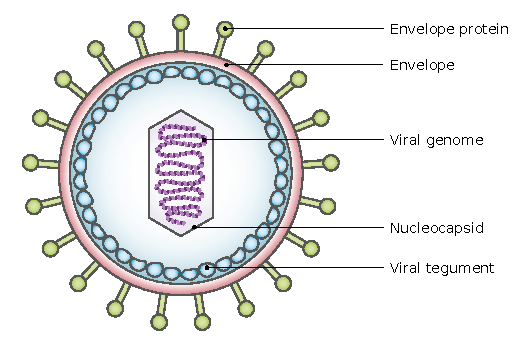
\includegraphics{Images/Viral_Tegument.pdf}}}
        \end{center}
    \column{0.45\textwidth}
        \vspace{-1.0em}
        \begin{center}
            \onslide<5->{\resizebox{1.0\linewidth}{!}{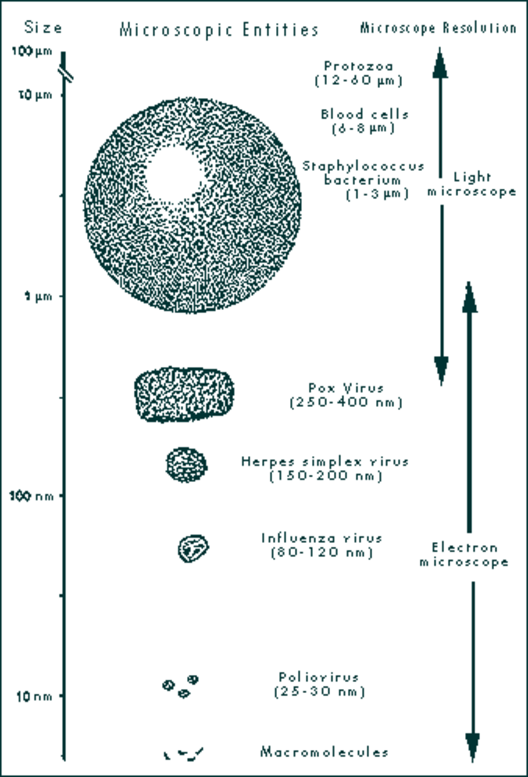
\includegraphics{Images/microentities338x497.pdf}}}
        \end{center}
    \end{columns}}

\end{frame}

\begin{frame}{Life Cycle of a Virus}

	\begin{center}
	\resizebox{0.8\linewidth}{!}{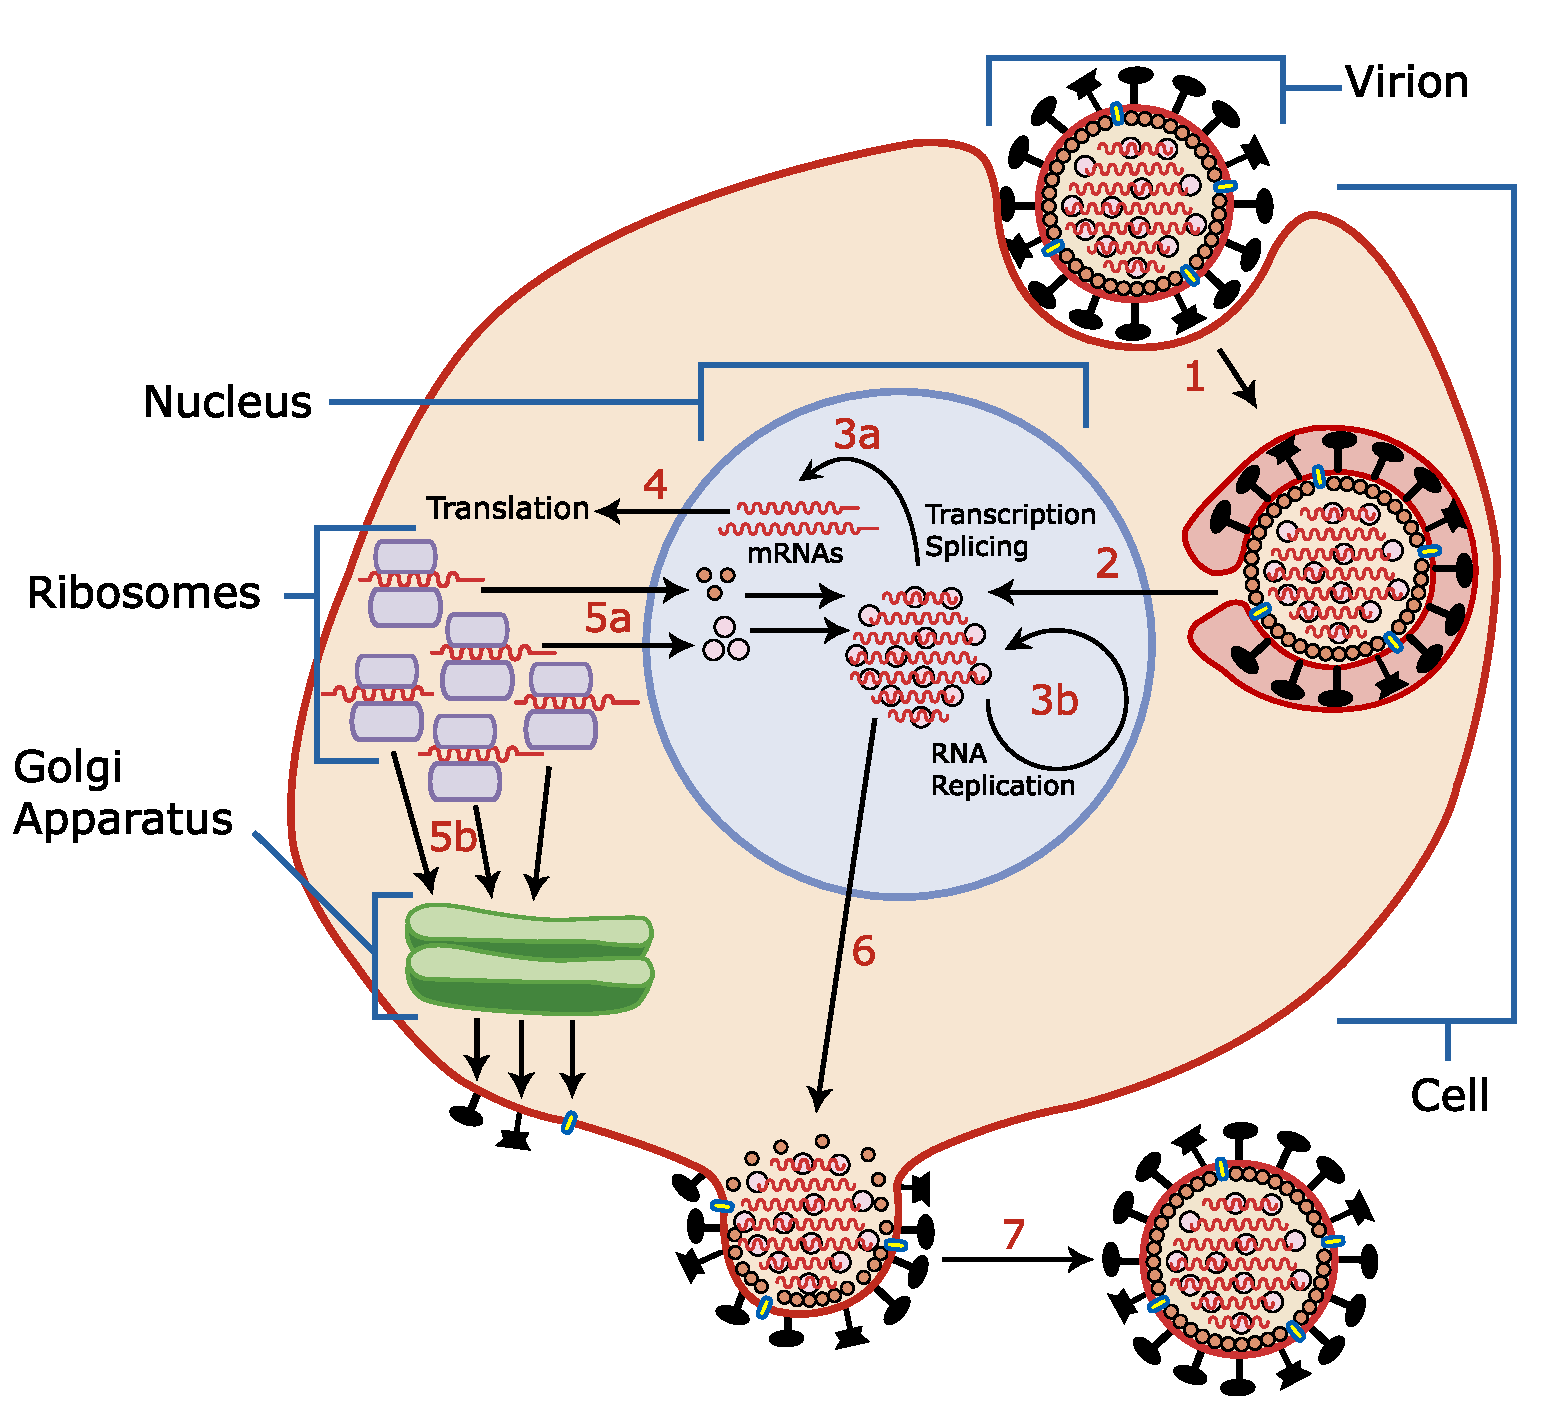
\includegraphics{Images/Virus_Replication_large.pdf}}
	\end{center}

\end{frame}

\begin{frame}{Experimental Virus Work}

    \begin{itemize} 
        \item<2-> Assay - an experiment for assessing or measuring characteristics of a substance
        \item<3-> Plaque assay
    \end{itemize}

    \resizebox{1.0\linewidth}{!}{\begin{columns}[T]
    \column{0.70\textwidth}
	\begin{center}
	\only<2-3>{\resizebox{1.0\linewidth}{!}{
\includegraphics{Images/petri_figure/petri_figureblank.pdf}}}

	\only<4>{\resizebox{1.0\linewidth}{!}{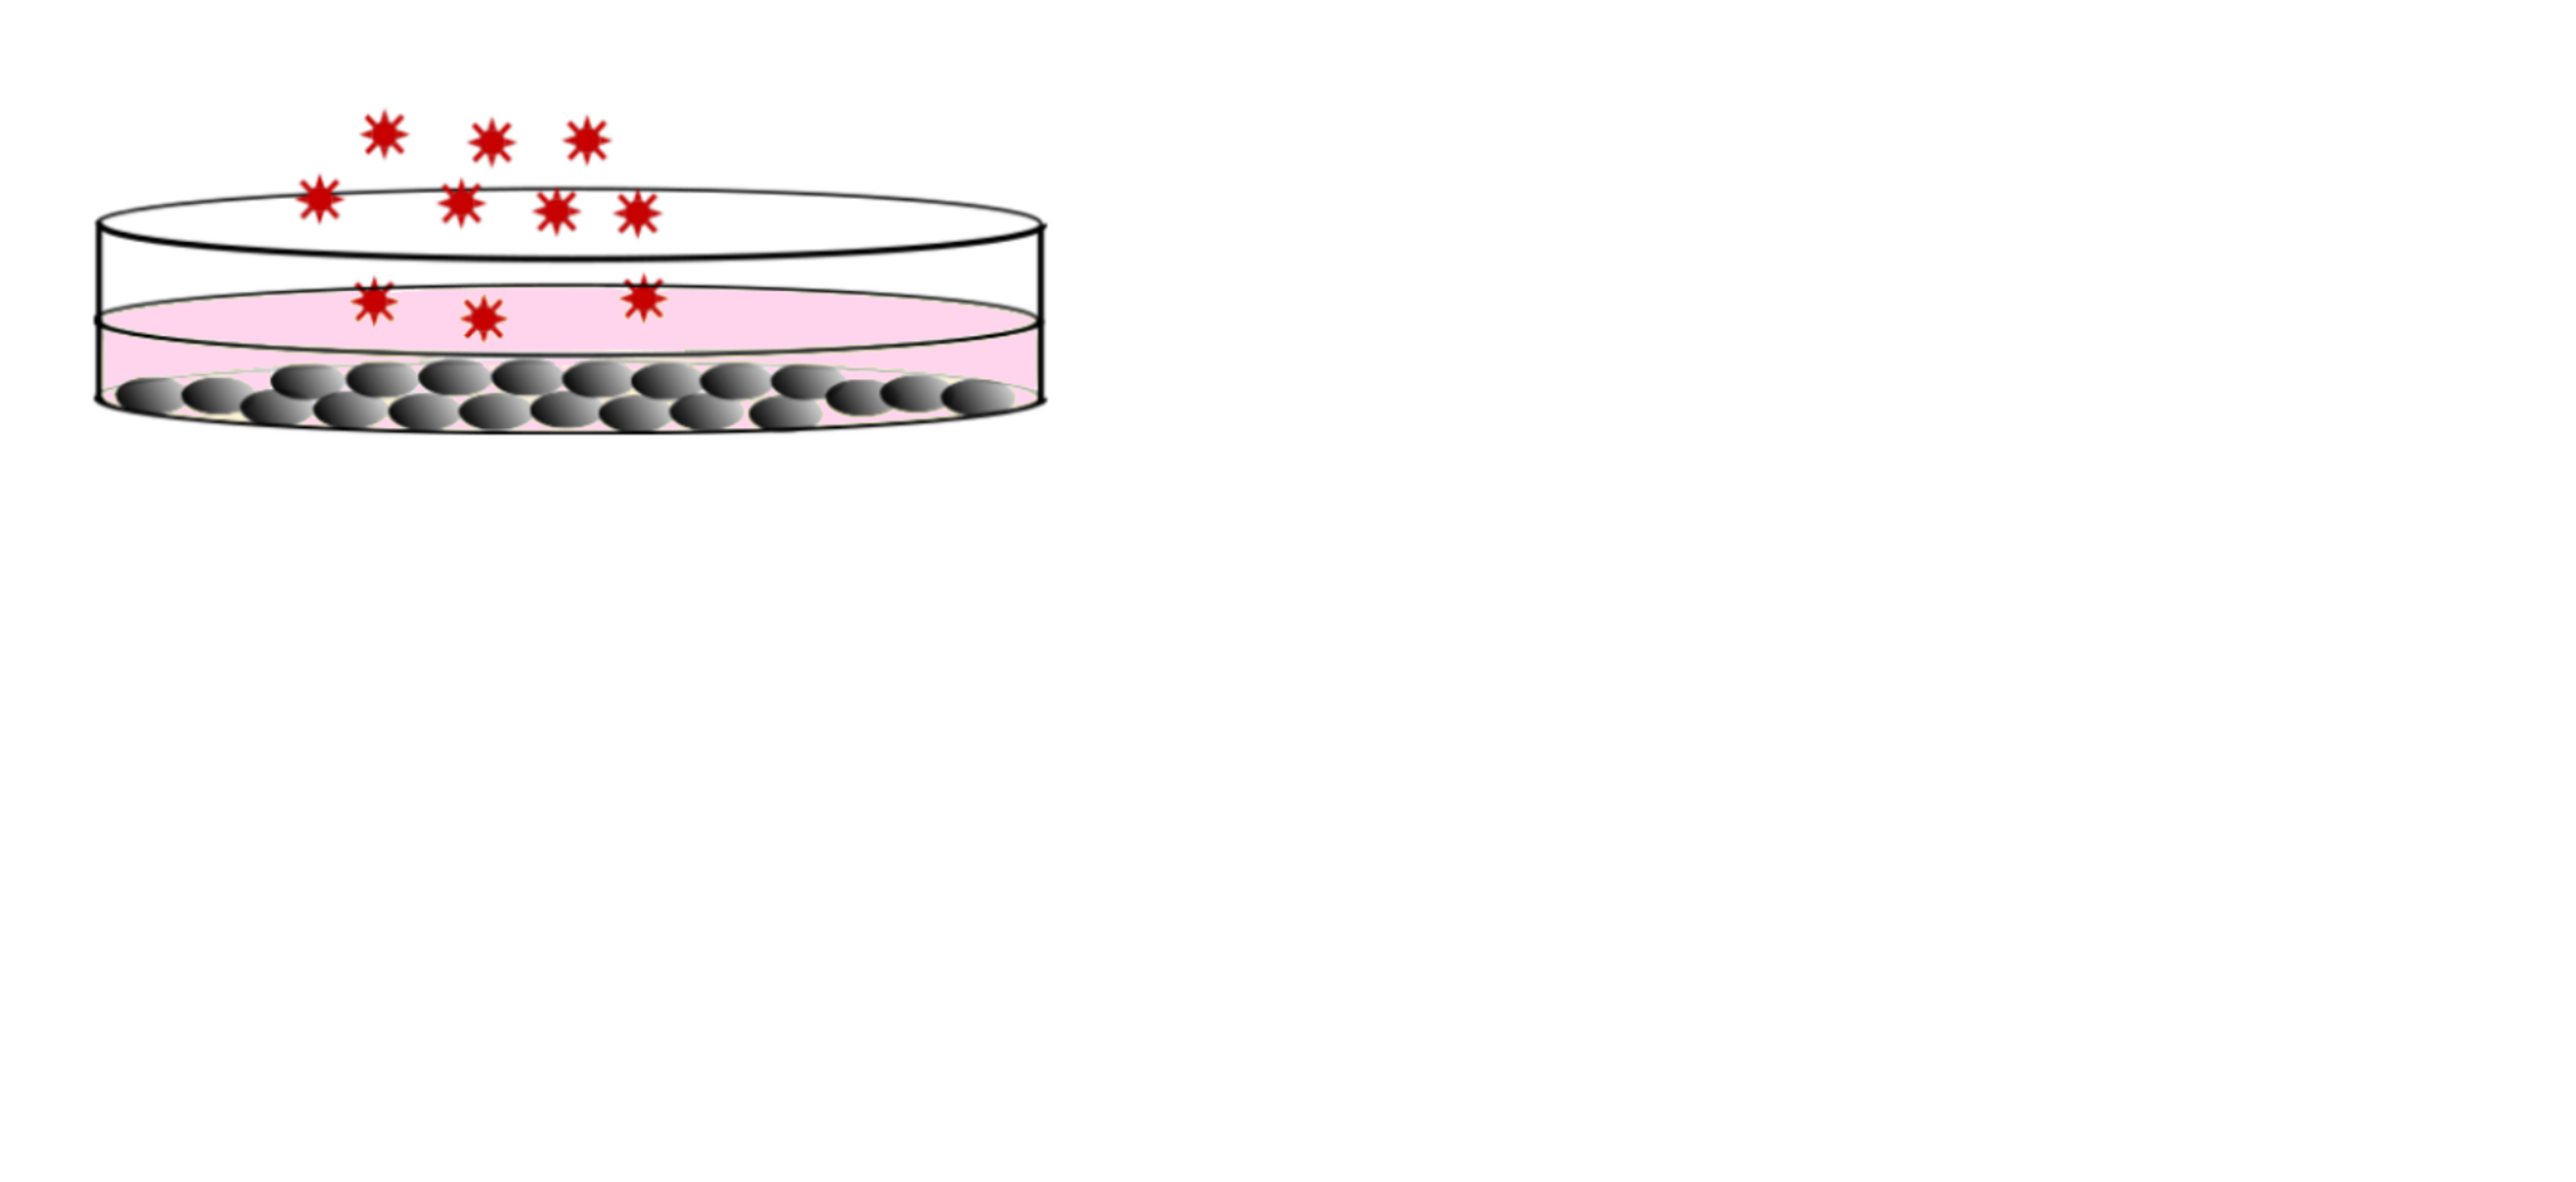
\includegraphics{Images/petri_figure/petri_figure1_pink.pdf}}}

	\only<5>{\resizebox{1.0\linewidth}{!}{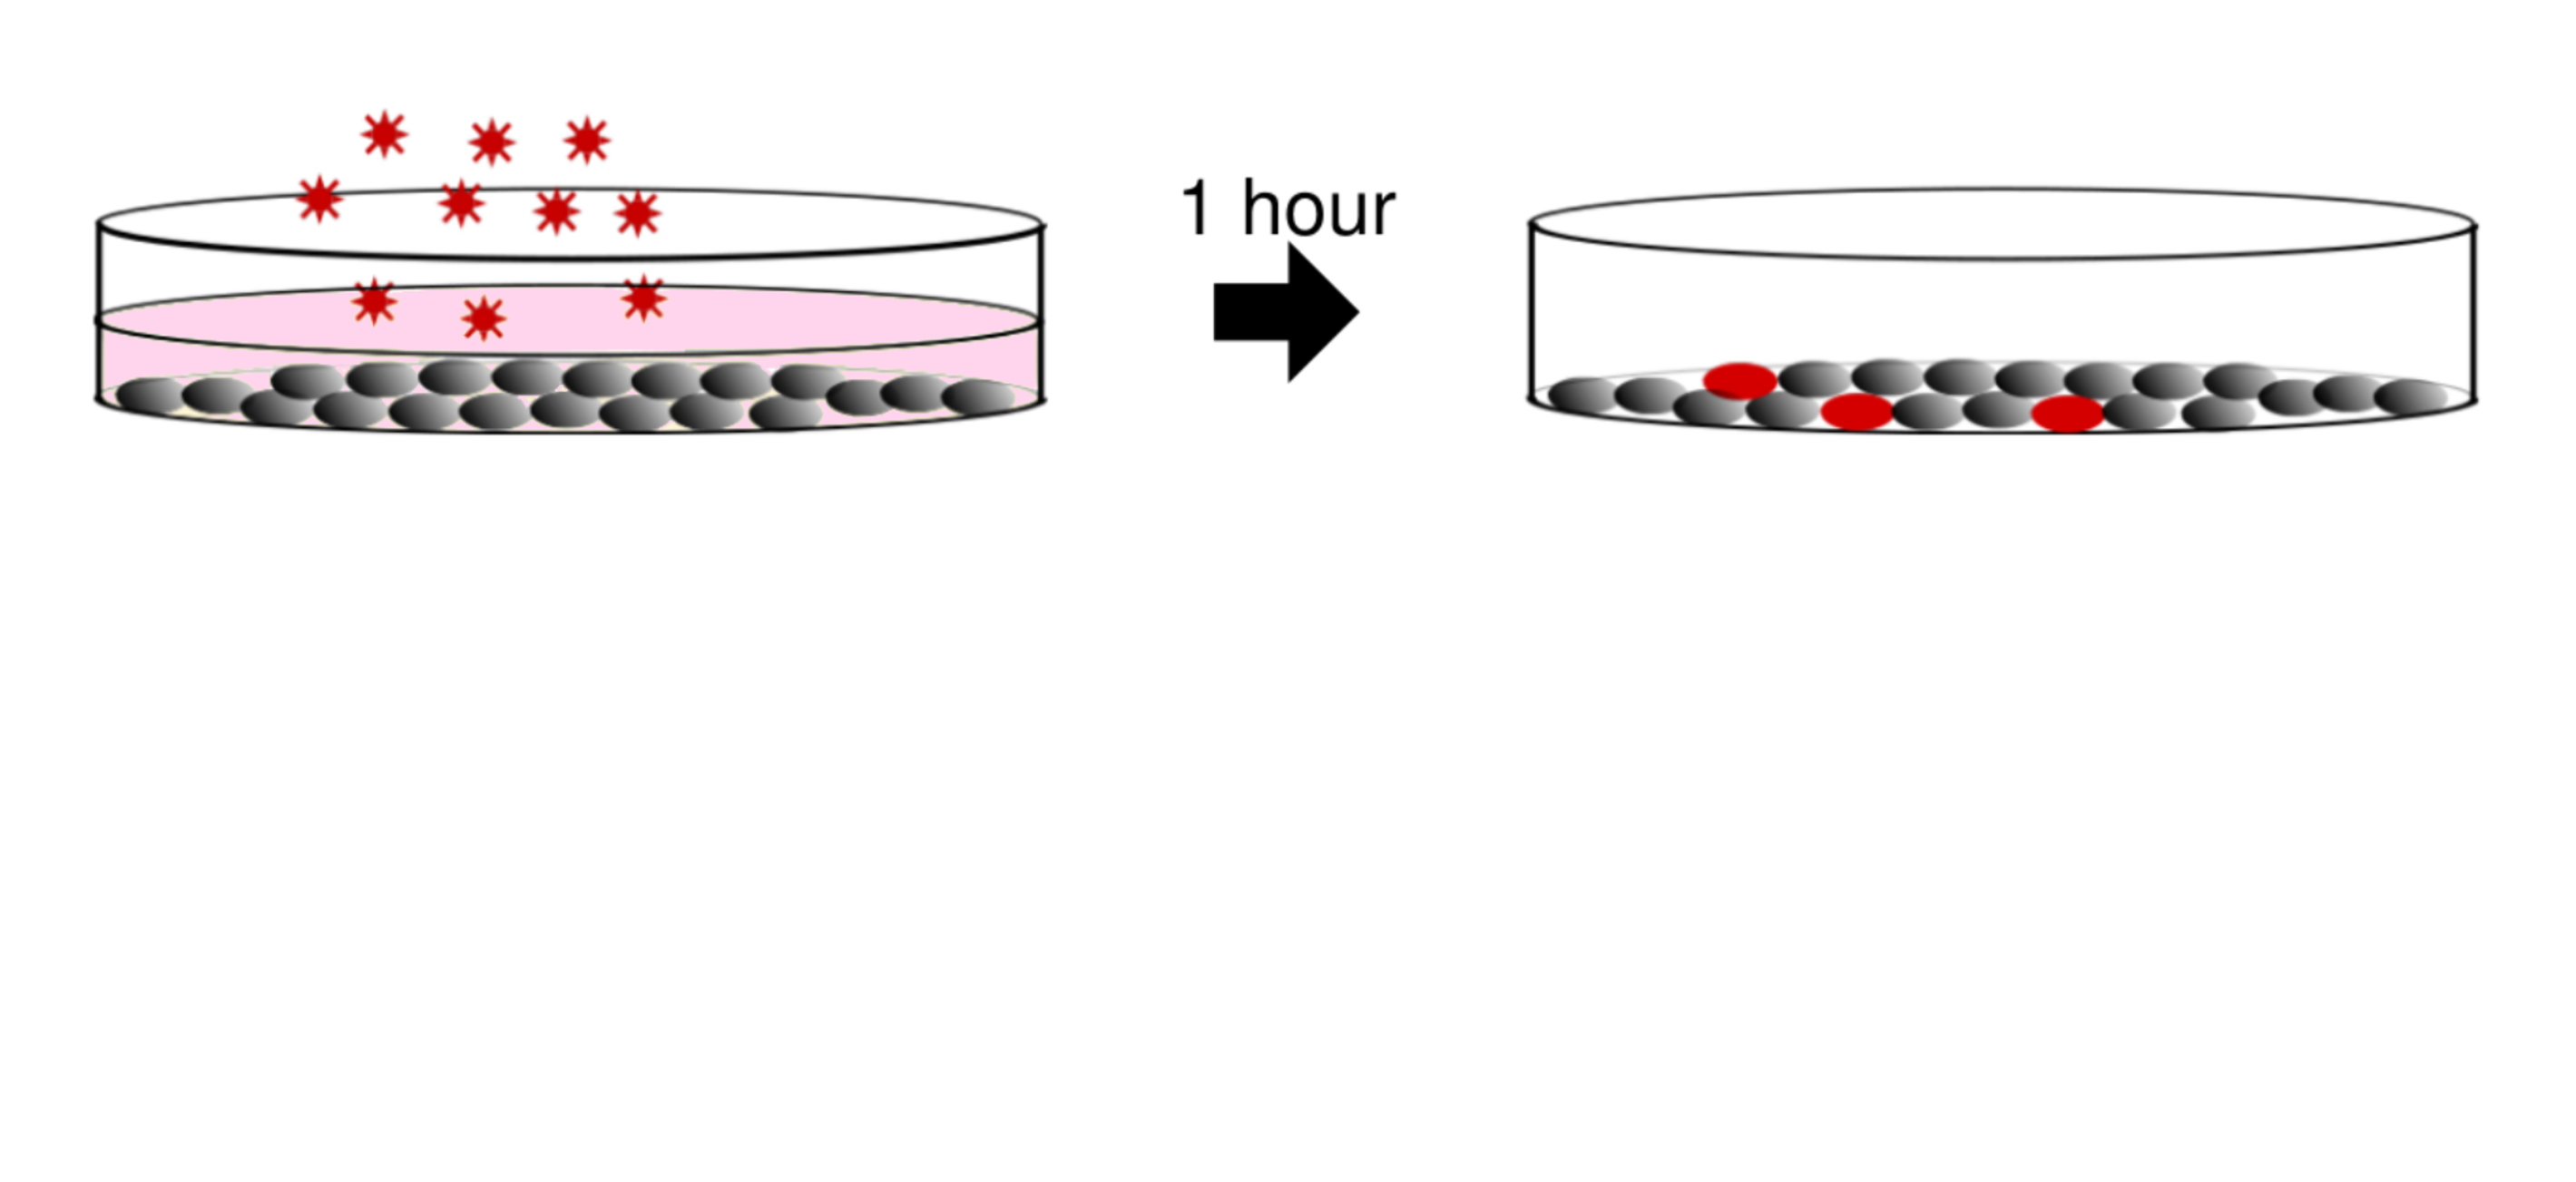
\includegraphics{Images/petri_figure/petri_figure2_pink.pdf}}}

	\only<6>{\resizebox{1.0\linewidth}{!}{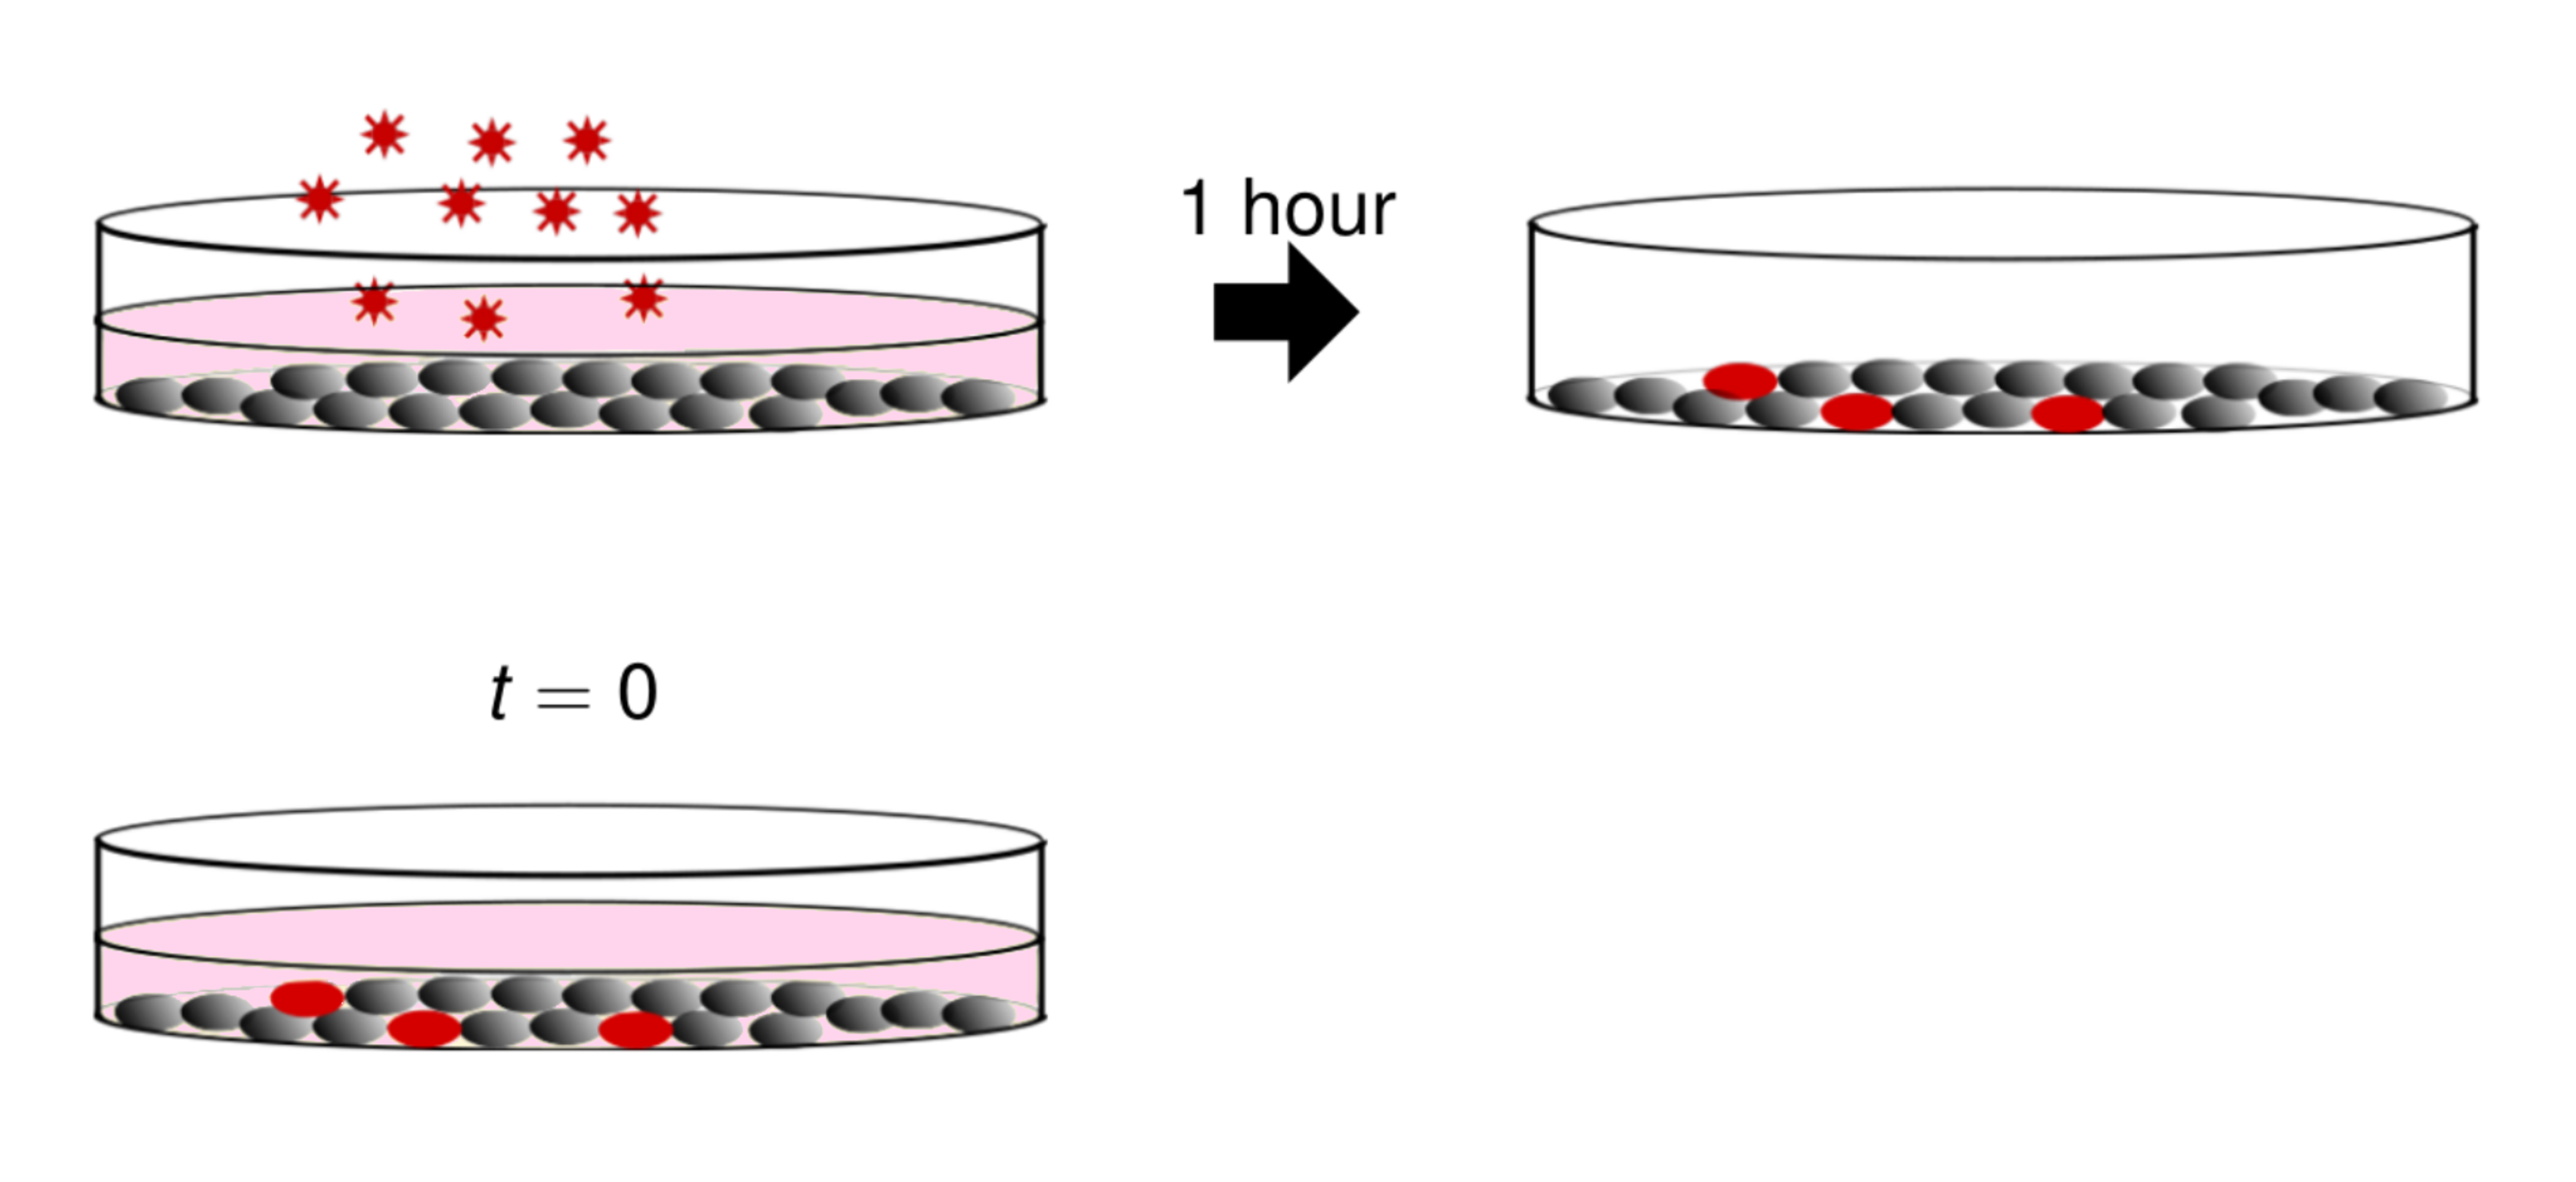
\includegraphics{Images/petri_figure/petri_figure3_pink.pdf}}}

	\only<7->{\resizebox{1.0\linewidth}{!}{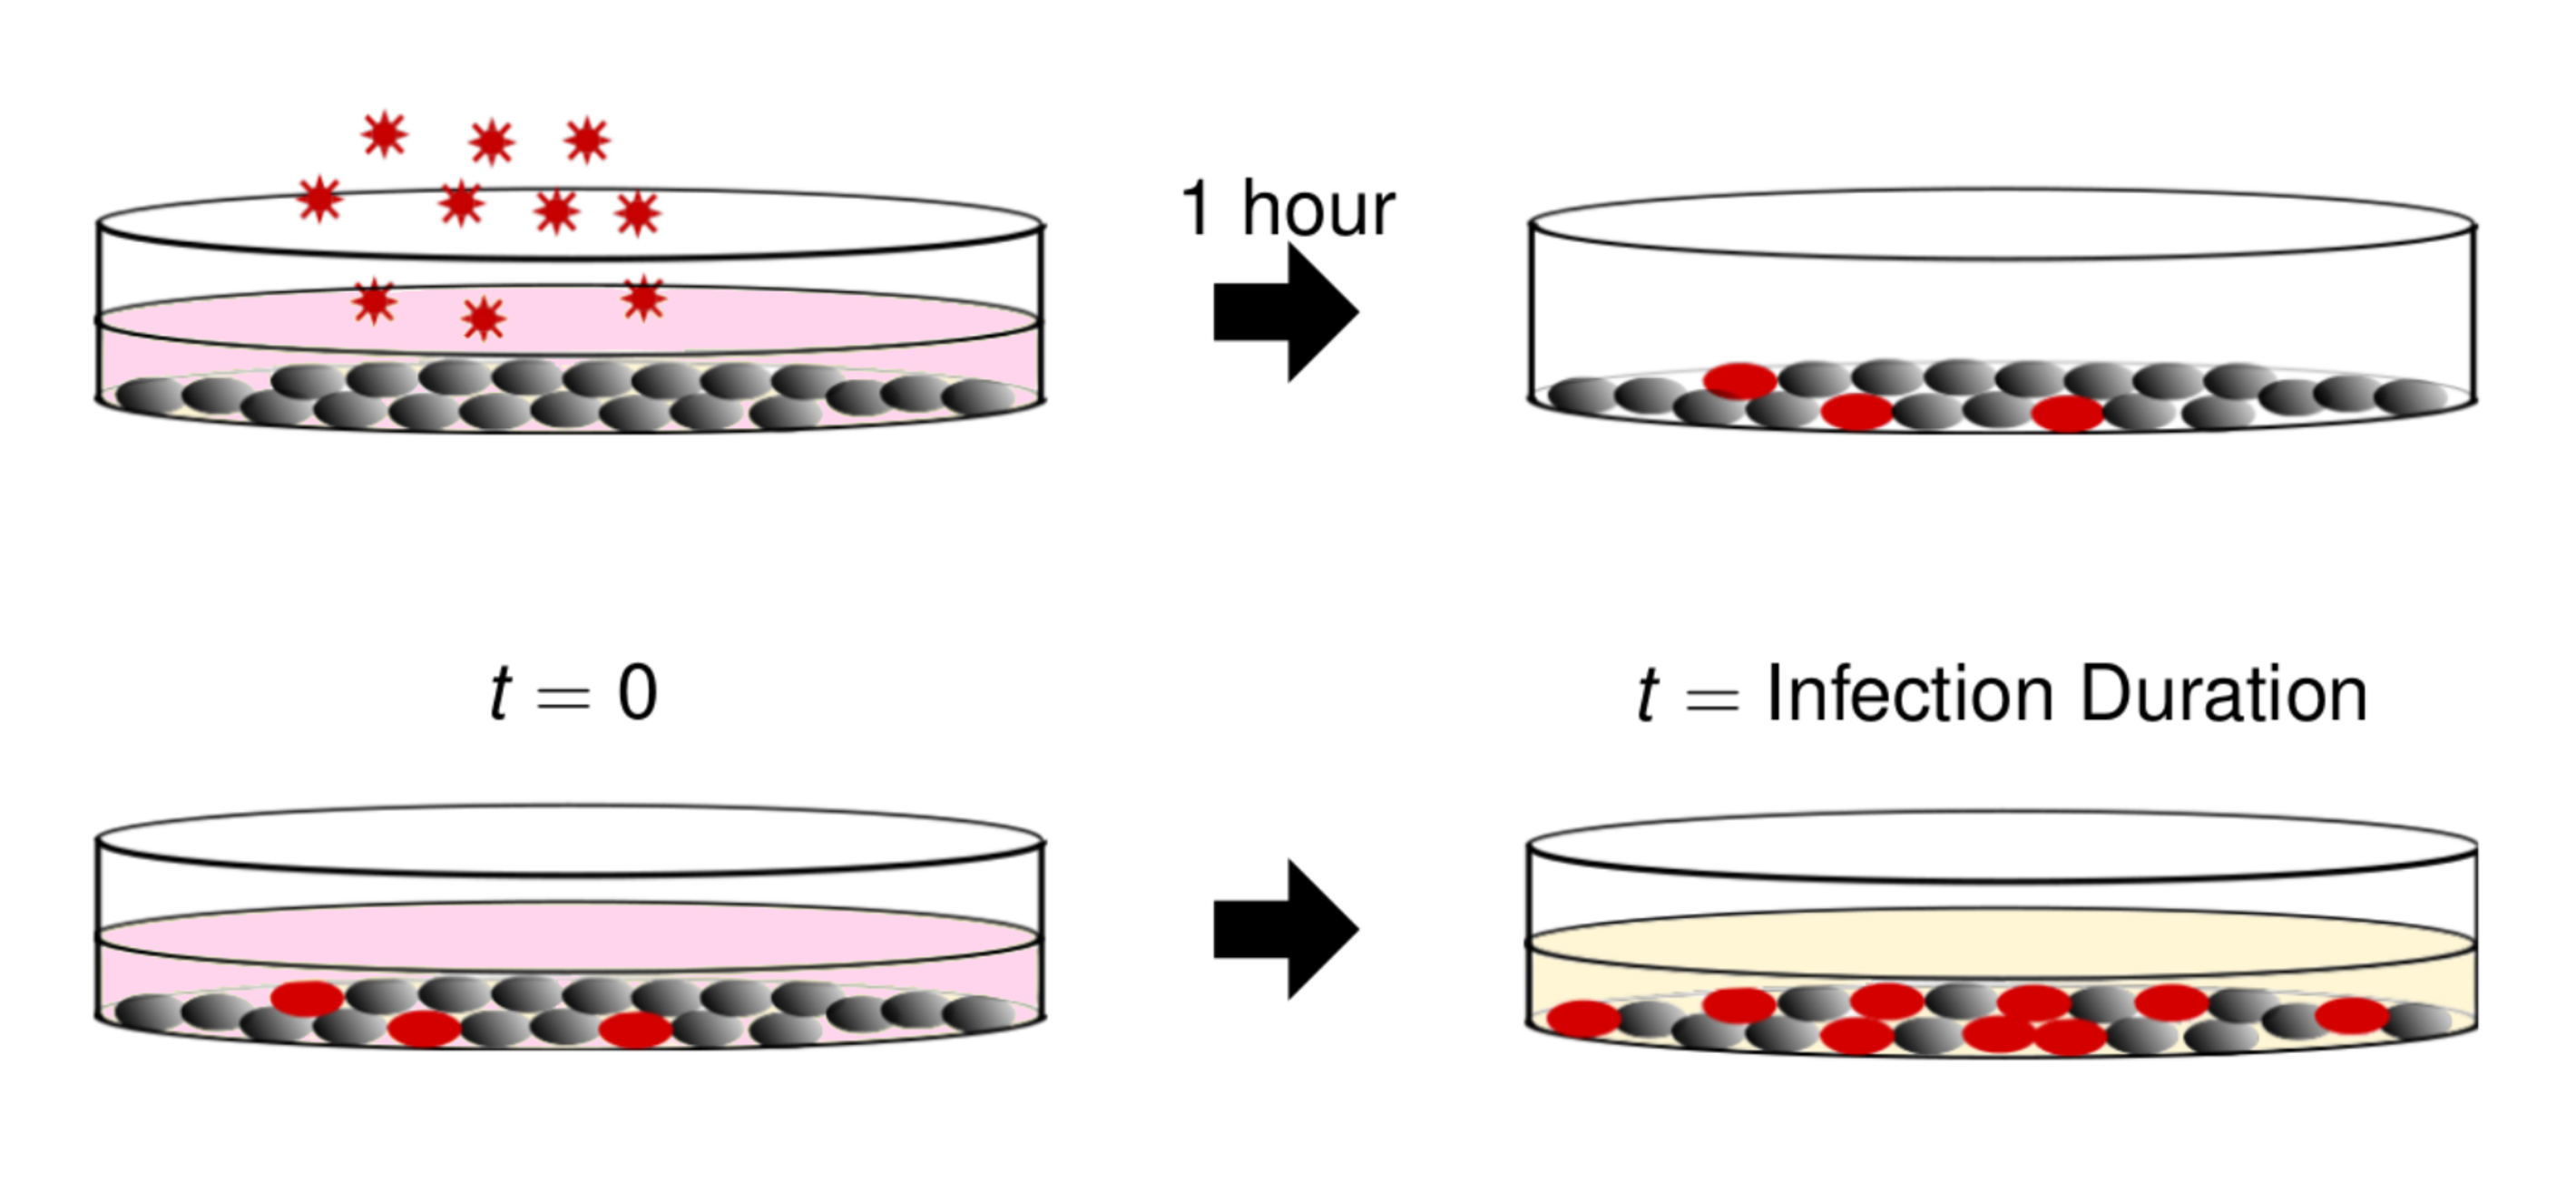
\includegraphics{Images/petri_figure/petri_figure_pink.pdf}}}
	\end{center}

    \column{0.30\textwidth}
	\begin{center}
	\onslide<8->{\resizebox{1.0\linewidth}{!}{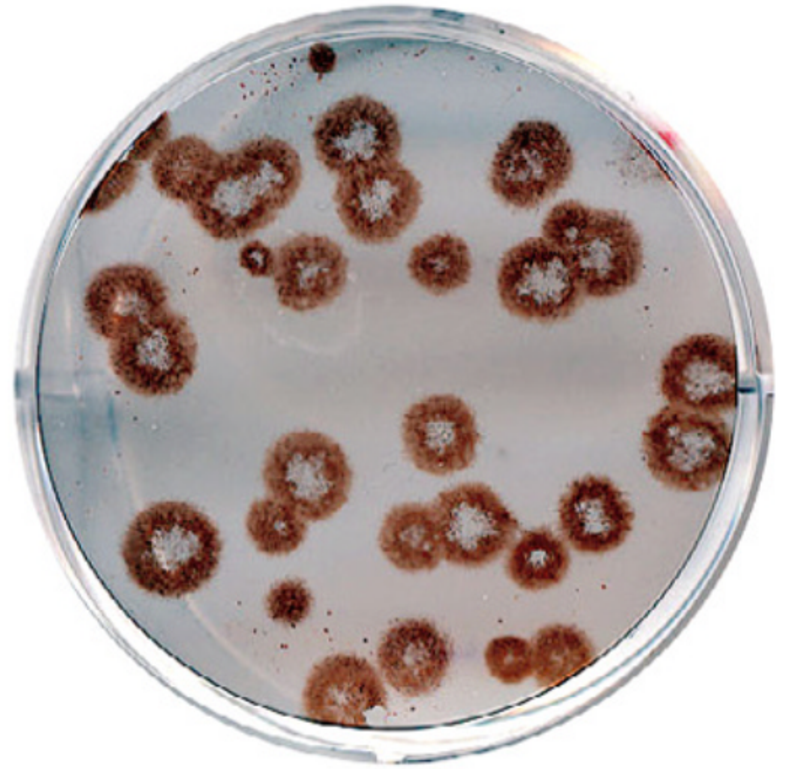
\includegraphics{Images/plaques.pdf}}}
	\end{center}

    \end{columns}}

\end{frame}

\begin{frame}{Viral Transmission}

    \begin{itemize}
        \item<2-> Viral transmission is the process by which viruses spread between cells 
    \end{itemize}

    \begin{itemize}    
        \item<3-> Aspects that affect viral transmission 
            \begin{itemize}
                \item[--]<4-> Transmission Modes
%                    \begin{itemize}
%                        \item[$\cdot$]<5-> Cell free transmission
%                        \item[$\cdot$]<6-> Cell to cell transmission
%                    \end{itemize}
                \item[--]<5-> Syncytia
%                    \begin{itemize}
%                        \item[$\cdot$]<8-> Multi-nucleated cells
%                    \end{itemize}
                \item[--]<6-> Advection
%                    \begin{itemize}
%                        \item[$\cdot$]<10-> Transfer of matter by the flow of a mucus
%                    \end{itemize}
            \end{itemize}    
    \end{itemize}

    \begin{itemize}
        \item<7-> Why this matters
        \begin{itemize}
            \item[--]<8-> Determines how quickly and far the virus spreads
            \item[--]<9-> Affects how the immune response interacts with the virus 
            \item[--]<10-> Affects if viral treatment reaches the virus
        \end{itemize}
    \end{itemize}

\end{frame}

\begin{frame}{Cell Free Transmission Mode}

\begin{center}
\resizebox{1.0\linewidth}{!}{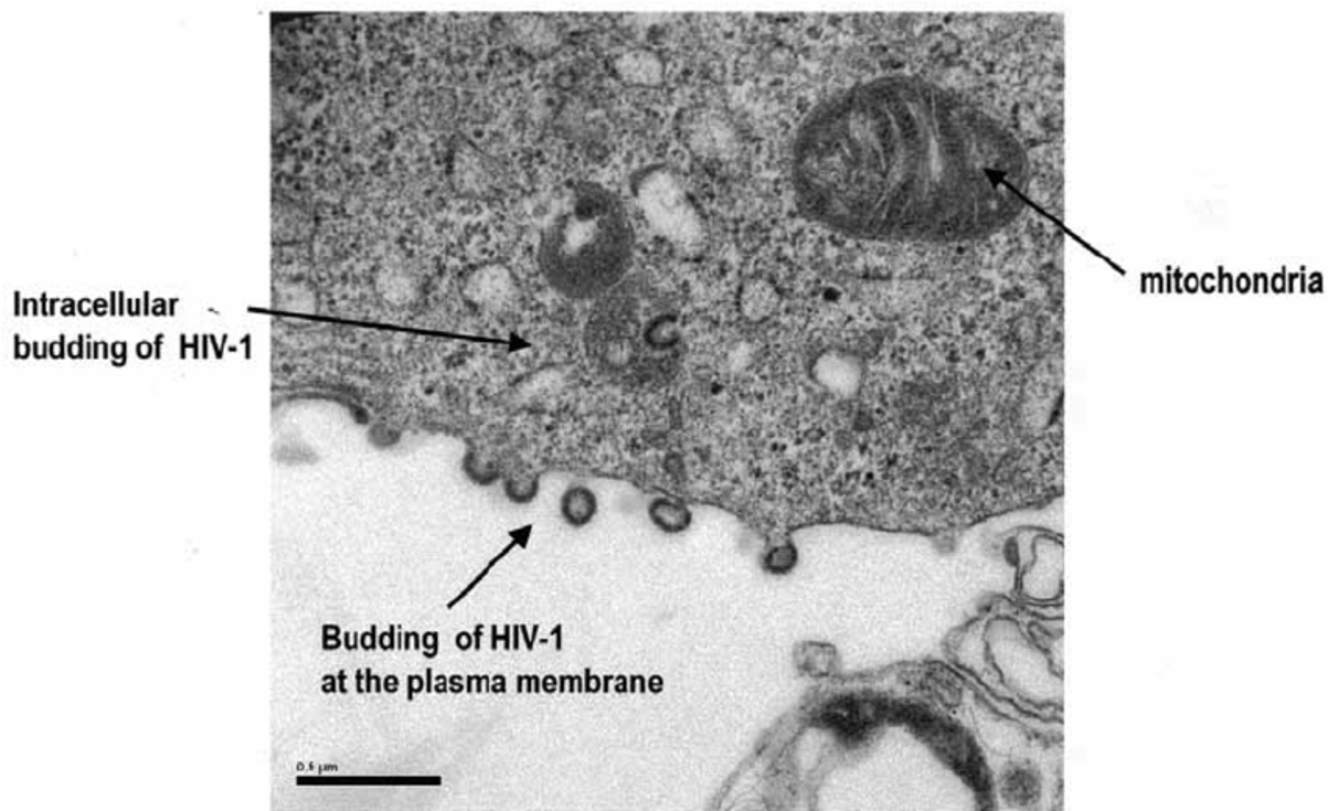
\includegraphics{Images/Electron-microscopy-thin-section-of-293J-cells-expressing-HIV-1.pdf}}
\end{center}

\end{frame}

\begin{frame}{Cell to Cell Transmission Mode}

\begin{center}
\resizebox{1.0\linewidth}{!}{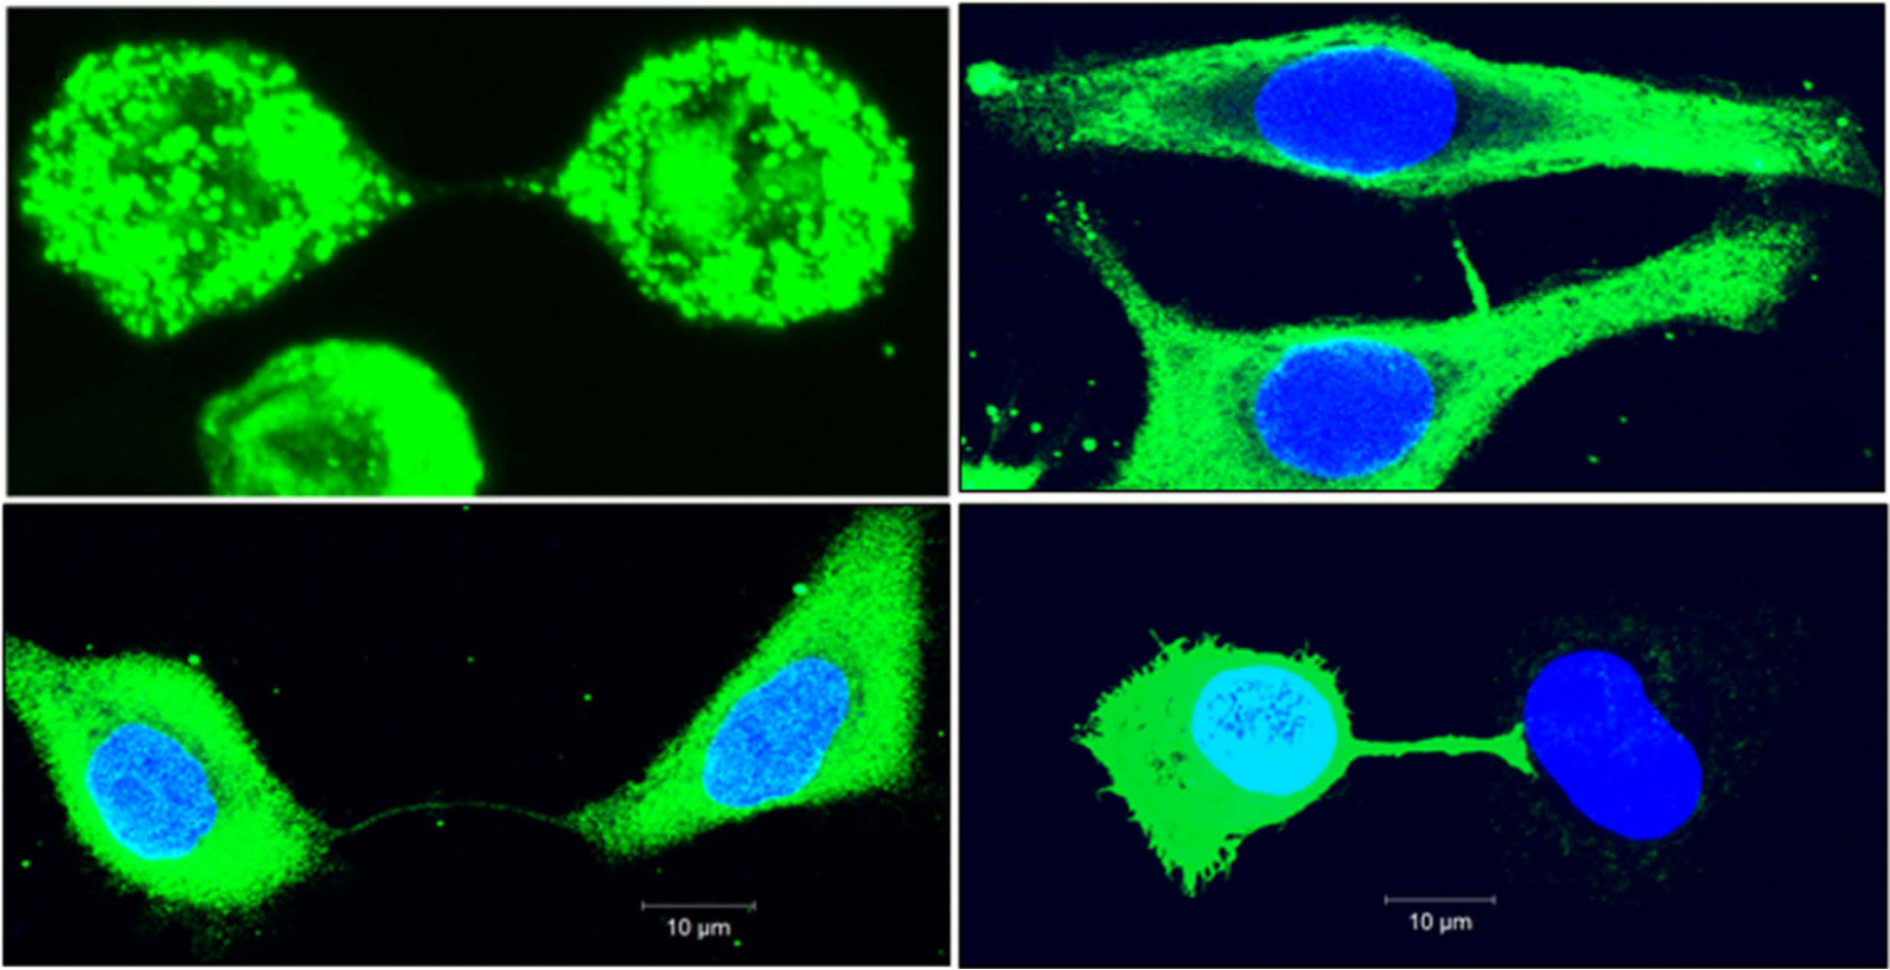
\includegraphics{Images/cell2cell.pdf}}
\end{center}

\end{frame}

\begin{frame}{Syncytia}
	\begin{center}
	\resizebox{0.75\linewidth}{!}{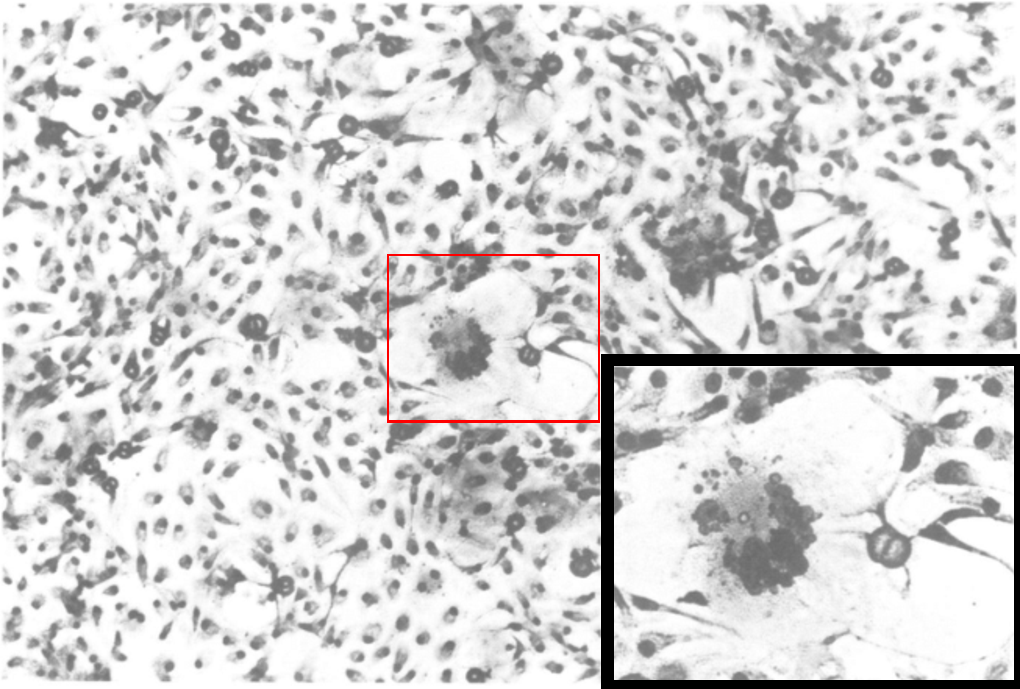
\includegraphics{Images/real.pdf}}
	\end{center}    

    \vspace{-2em}

\newcolumntype{g}{>{\columncolor{gray!25}}c}
\onslide<2->{
\begin{table}[h]
    \centering
    \resizebox{1.0\linewidth}{!}{
    \begin{tabular}{|g|c|c|}
        \hline
        \rowcolor{gray!25}
          & \onslide<2->{Produces More Virus} & \onslide<3->{Produces Less Virus}\\
        \hline
        \onslide<4->{Longer Life Span} & \onslide<6->{More Severe Infection} & \onslide<7->{Unknown difference in Severity}\\
        \hline
        \onslide<5->{Shorter Life Span} & \onslide<7->{Unknown difference in Severity} & \onslide<8->{Less Severe Infection}\\
        \hline
    \end{tabular}}
\end{table}
}

\end{frame}

\begin{frame}{Advection}

    \resizebox{1.0\linewidth}{!}{\begin{columns}
    \column{0.45\textwidth}
    \begin{itemize}
        \item<2-> Virus enters through the upper respiratory tract
        \item<3-> The virus diffuses through the mucus 
        \item<5-> Advection upwards away from the lower respiratory tract 
    \end{itemize}

    \column{0.45\textwidth}
    \begin{center}
    \onslide<1->{\resizebox{1.0\linewidth}{!}{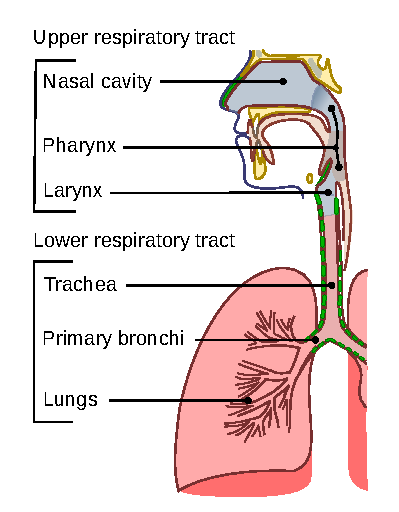
\includegraphics{Images/Illu_conducting_passages.pdf}}}
    \end{center}
    \end{columns}}

\end{frame}

\begin{frame}{Advection}
    
    \begin{center}
    \only<2->{\resizebox{0.8\textwidth}{!}{\animategraphics[autoplay]{20}{Images/Cilia/Ciliary}{100}{425}}}
    \only<1>{\resizebox{0.8\linewidth}{!}{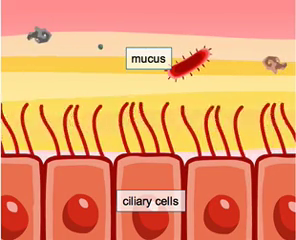
\includegraphics{Images/Cilia/Ciliary100.png}}}
    \end{center} 

\end{frame}


\begin{frame}{Gaps in Current Research}

    \vspace{-2.0em}
    \resizebox{1.0\linewidth}{!}{\begin{columns}[t]
    \column{0.33\textwidth}
    \begin{center}
        \onslide<2->{Transmission Modes}
    \end{center}

    \column{0.34\textwidth}
    \begin{center}
        \onslide<6->{Syncytia}
    \end{center}

    \column{0.33\textwidth}
    \begin{center}    
        \onslide<8->{Advection}
    \end{center}
    \end{columns}}

    \vspace{-1.75em}
    
    \resizebox{1.0\linewidth}{!}{\begin{columns}[t]
    \column{0.33\textwidth}
    \begin{center}
        \onslide<2->{\fbox{\parbox{\textwidth}{\begin{itemize}
            \item<3-> ODE
            \item<4-> Stochastic Model
        \end{itemize}}}}
        \onslide<5->{\fbox{\parbox{\textwidth}{\begin{itemize}
            \item<5-> No spatial dependence
        \end{itemize}}}}

        \onslide<12->{\arrowdown} 
    \end{center}

    \column{0.34\textwidth}
    \begin{center}
        \onslide<6->{\fbox{\parbox{\textwidth}{\begin{itemize}
            \vspace{2.75em}            
            \item[]<7-> No published models
            \vspace{2.75em}
        \end{itemize}}}}

        \onslide<12->{\arrowdown}
    \end{center}

    \column{0.33\textwidth}
    \begin{center}
        \onslide<8->{\fbox{\parbox{\textwidth}{\begin{itemize}
            \item<9-> ODE
            \item<10-> 1D PDE 
        \end{itemize}}}}
        \onslide<11->{\fbox{\parbox{\textwidth}{\begin{itemize}
            \item<11->  No/Very simple spatial dependence
        \end{itemize}}}}

        \onslide<12->{\arrowdown}
    \end{center}
    \end{columns}}

    \resizebox{1.0\linewidth}{!}{\begin{columns}[t]
    \column{1.0\textwidth}
        \onslide<12->{\fbox{\parbox{\textwidth}{\begin{center}
        \onslide<13->{Develop model that includes spatial dependence}
        \end{center}}}}
    \end{columns}}

\end{frame}

%-----------------------------------------------------------------------------------
\section{Methods}

\begin{frame}{Modeling Spatial Dependence}

    \onslide<2->{
    \resizebox{1.0\linewidth}{!}{\begin{columns}[T]
    \column{0.4375\textwidth}
    \begin{center} 
    \resizebox{1.0\linewidth}{!}{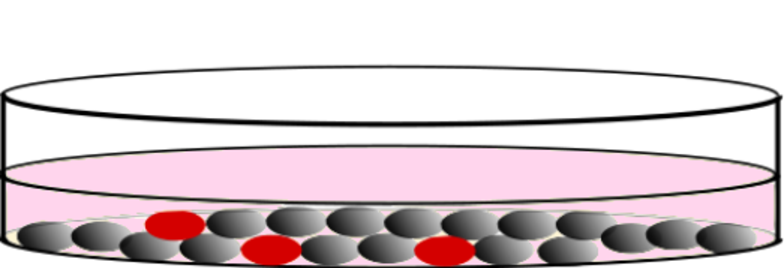
\includegraphics{Images/multiple_cycle_left_with_fluid_pink.pdf}}
    \end{center}

    \column{0.125\textwidth}
    \vspace{1.0em}
    \begin{center}
    \resizebox{1.0\linewidth}{!}{\fcolorbox{white}{white}{\parbox{\textwidth}{\begin{center}  
        \arrowright
    \end{center}}}}
    \end{center}

    \column{0.4375\textwidth}
    \begin{center} 
    \resizebox{1.0\linewidth}{!}{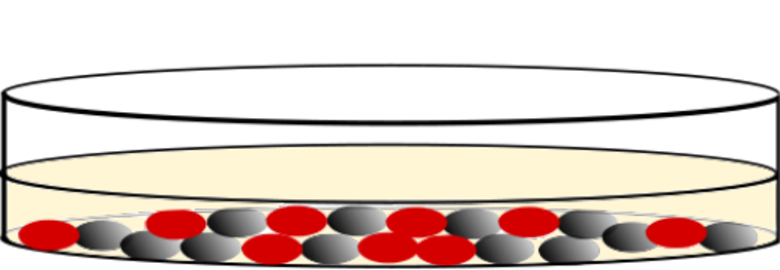
\includegraphics{Images/multiple_cycle_right_with_fluid.pdf}}
    \end{center}
    \end{columns}}}

\end{frame}

\begin{frame}{Modeling Spatial Dependence}

    \begin{center} 
    \resizebox{0.5\linewidth}{!}{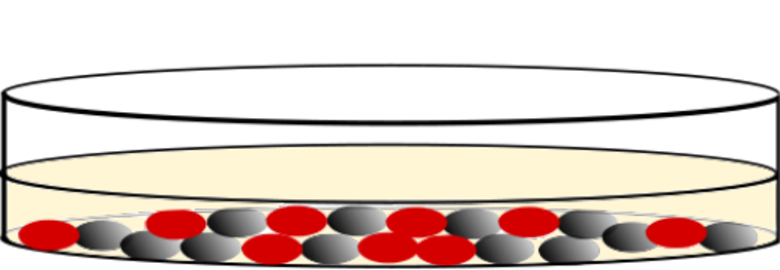
\includegraphics{Images/multiple_cycle_right_with_fluid.pdf}}
    \end{center}

    \vspace{-1.25em}
    \resizebox{1.0\linewidth}{!}{\begin{columns}
    \column{0.33\textwidth}

    \column{0.34\textwidth}
    \begin{center}     
        \onslide<2->{\arrowSW}
        \onslide<5->{\arrowSE}
    \end{center}

    \column{0.33\textwidth}

    \end{columns}}
    \vspace{0.25em}

    \resizebox{1.0\linewidth}{!}{\begin{columns}
    \column{0.45\textwidth}
    \resizebox{1.0\linewidth}{!}{\onslide<2->{\fbox{\parbox{\textwidth}{
    \begin{center} 
         \onslide<2->{Partial Differential Equation Model}
        \vspace{1em}

         \onslide<3->{$\frac{\partial V}{\partial t}=D \nabla^{2}V+pI-cV$}
    \end{center}
    \onslide<4->{\small $D =$ diffusion matrix}

    \onslide<4->{\small $p =$ production rate}

    \onslide<4->{\small $c =$ clearance rate}

    }}}}

    \column{0.45\textwidth}
    \resizebox{1.0\linewidth}{!}{\onslide<5->{\fbox{\parbox{\textwidth}{
    \begin{center}  
        \onslide<5->{Agent Based Model}
        \vspace{1em}
 
        \onslide<6->{\resizebox{0.6\linewidth}{!}{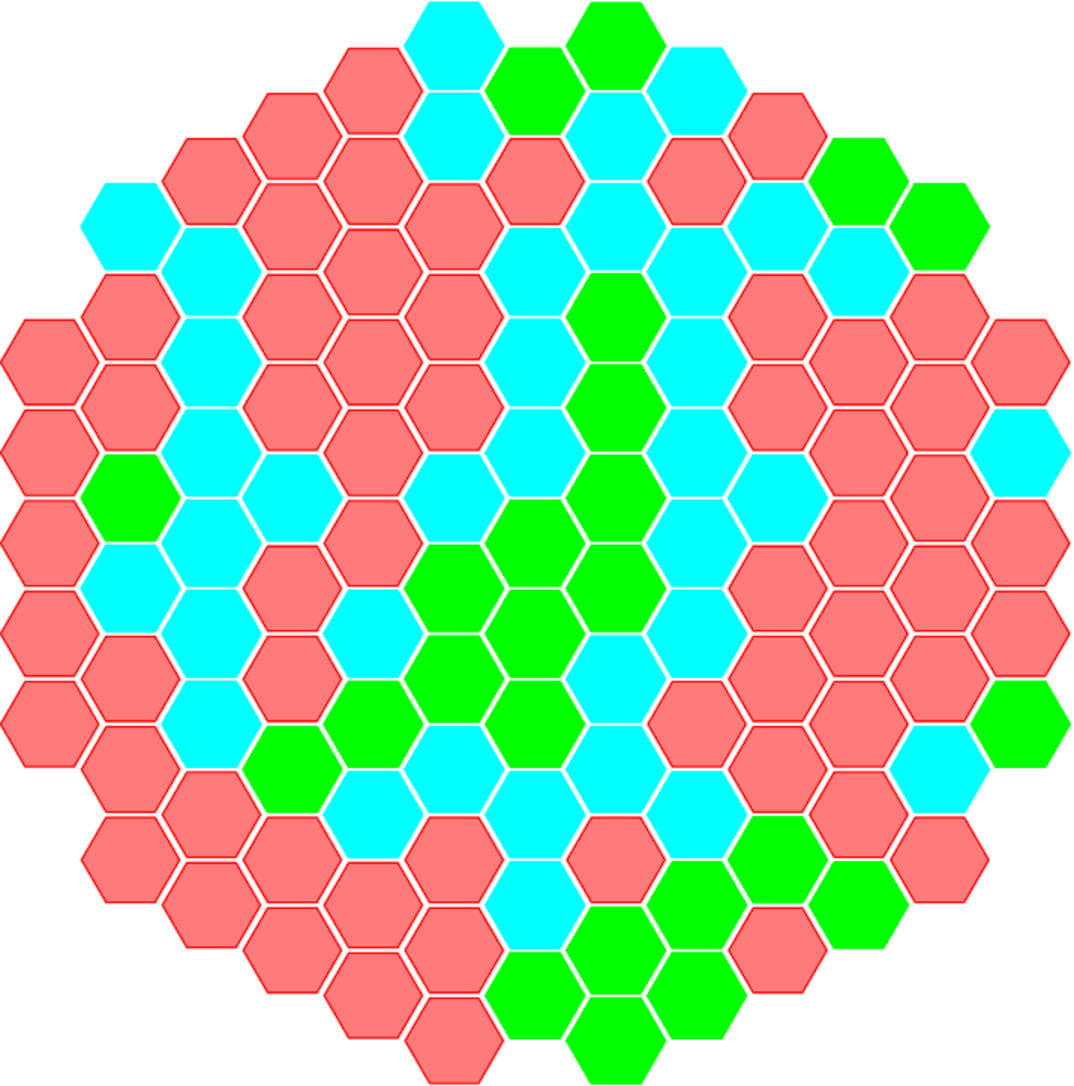
\includegraphics{Images/HEICells.pdf}}}
    \end{center}}}}}

    \end{columns}}

\end{frame}

\begin{frame}{Stages of Infection}
    
    \vspace{-1em}
    \onslide<2->{
    \resizebox{1.0\linewidth}{!}{\begin{columns}[T]
    \column{0.33\textwidth}
    \begin{center}
        \resizebox{1.0\linewidth}{!}{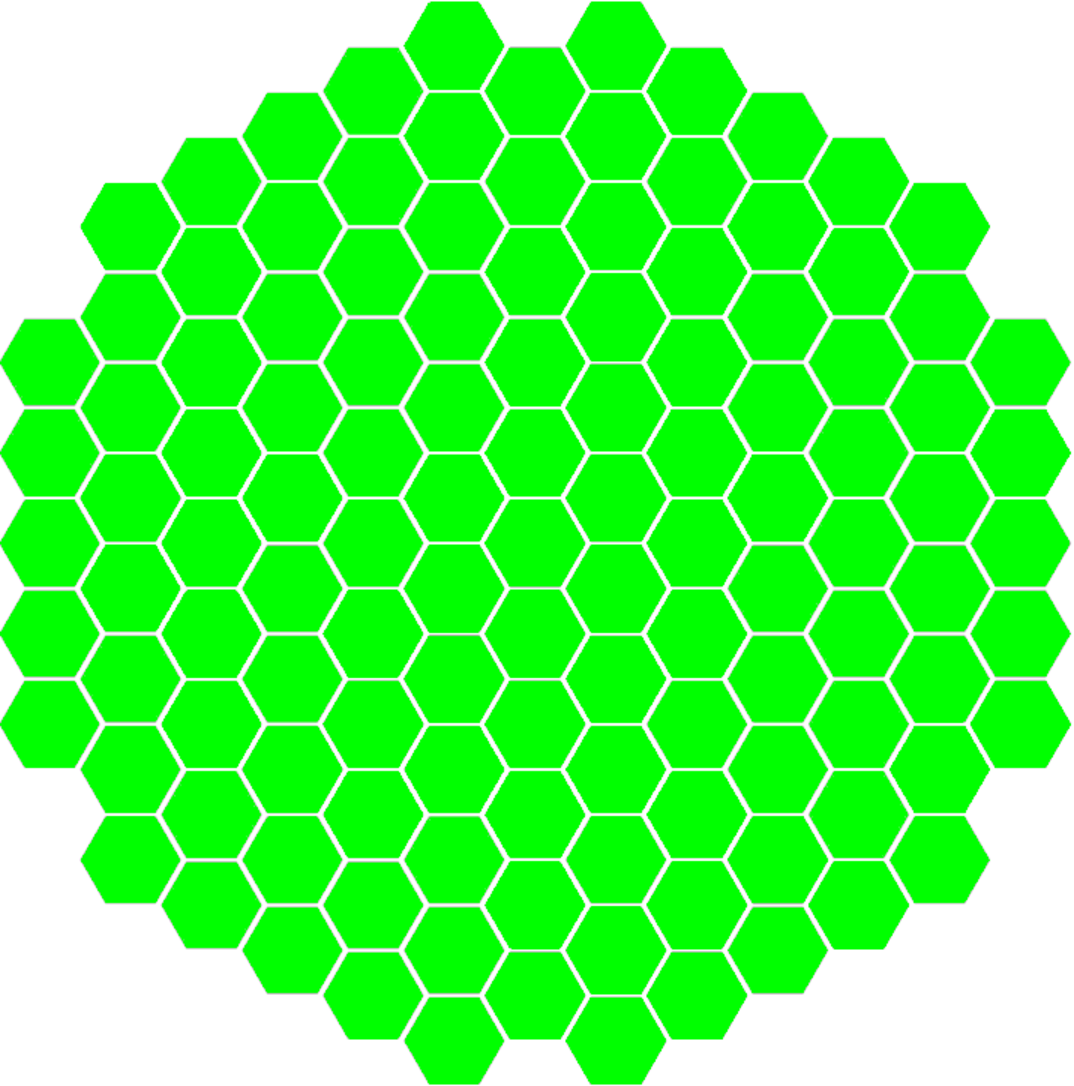
\includegraphics{Images/HCells1.pdf}}
    \end{center}

    \column{0.34\textwidth}
    \begin{center}
        \resizebox{1.0\linewidth}{!}{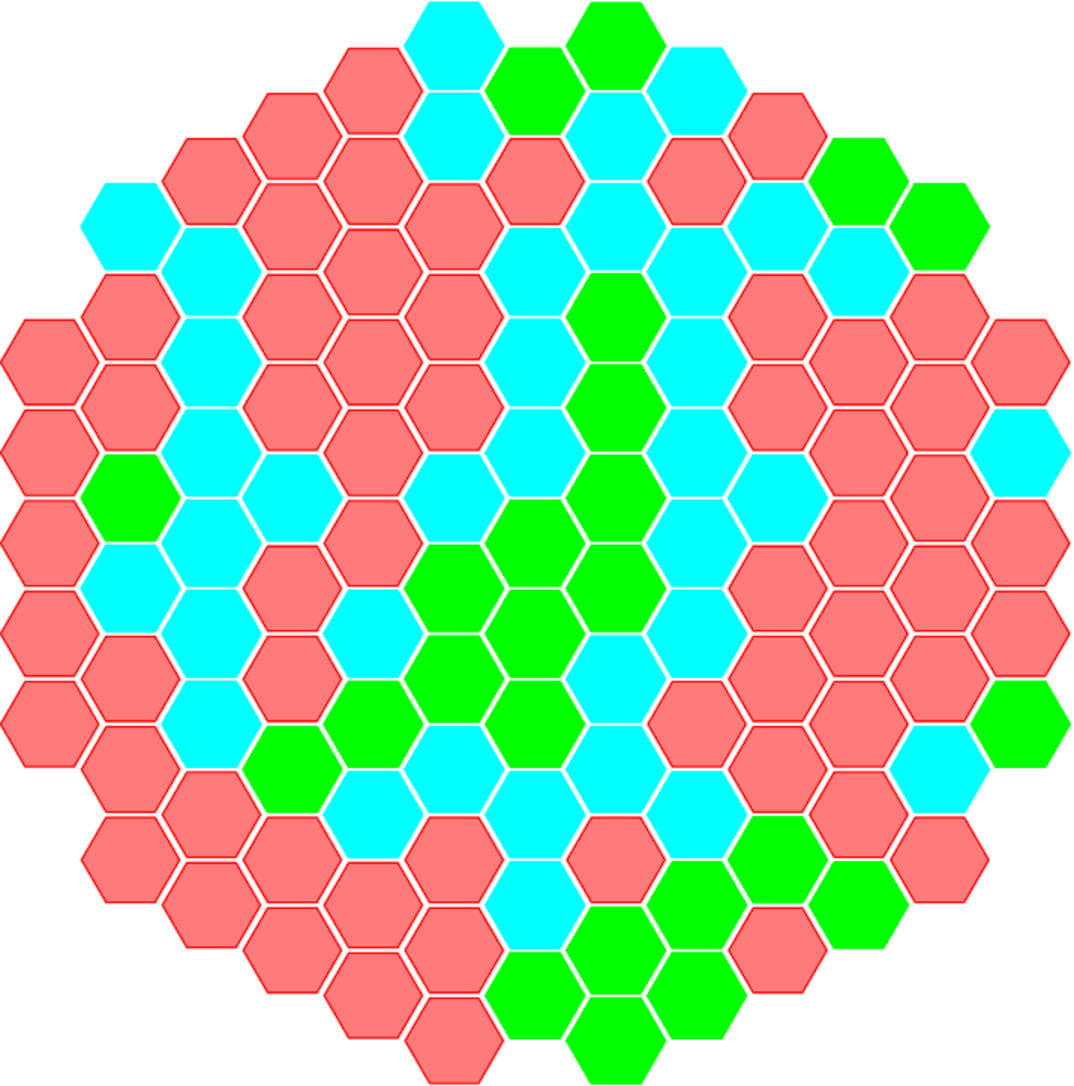
\includegraphics{Images/HEICells.pdf}}
    \end{center}

    \column{0.33\textwidth}
    \begin{center}
        \resizebox{1.0\linewidth}{!}{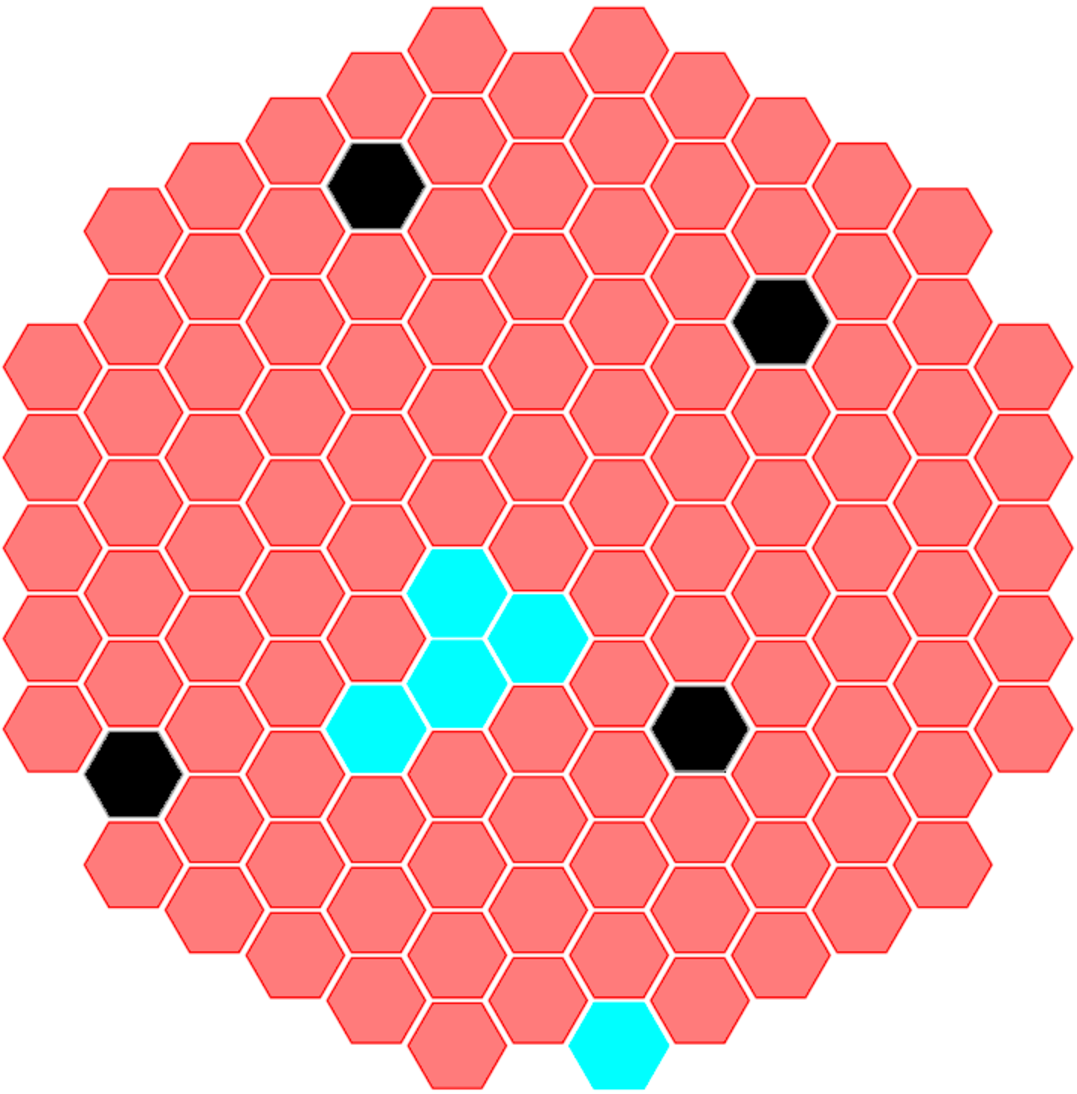
\includegraphics{Images/EIDCells.pdf}}
    \end{center}

    \end{columns}}}

    \vspace{1em}
    \definecolor{AGreen}{HTML}{00ff00}

    \begin{tikzpicture}
        \onslide<3->{\node[state, draw=AGreen, fill=AGreen!10] (H) {$Healthy$};}
        \onslide<4->{\node[state, draw=cyan, fill=cyan!10, right of=H] (E) {$Eclipse$};}
        \onslide<5->{\node[state, draw=red, fill=red!10, right of=E] (I) {$Infected$};}
        \onslide<6->{\node[state, draw=black, fill=black!10, accepting, right of=I] (D) {$Dead$};}
        
        \onslide<4->{\draw   (H) edge[above] node{} (E);}
        \onslide<5->{\draw   (E) edge[above] node{$\tau_E$} (I);}
        \onslide<6->{\draw   (I) edge[above] node{$\tau_I$} (D);}
    \end{tikzpicture}

\end{frame}

\begin{frame}{Transmission Mode}

    \resizebox{1.0\linewidth}{!}{\begin{columns}[T]
    \column{0.60\textwidth}
    \onslide<2->{Probability of a Cell Free Infection}
    \begin{itemize}
        \item<2-> $\mathrm{P_{cf}} = V \beta \Delta t$
            \begin{itemize}
                \item[--]<3-> $V$ is the amount of virus that is above a cell
                \item[--]<3-> $\beta$ is the infection rate of virus
                \item[--]<3-> $\Delta t$ is the time-step of the simulation
            \end{itemize}
    \end{itemize}
    \onslide<6->{Probability of a cell to cell Infection}
    \begin{itemize}
        \item<6-> $\mathrm{P_{c2c}} = x$ 
            \begin{itemize}
                \item[--]<7-> $x$ is a fixed number between 0 and 1
            \end{itemize}
    \end{itemize}

    \column{0.40\textwidth}
    \begin{center}
    \only<4>{\resizebox{1.0\linewidth}{!}{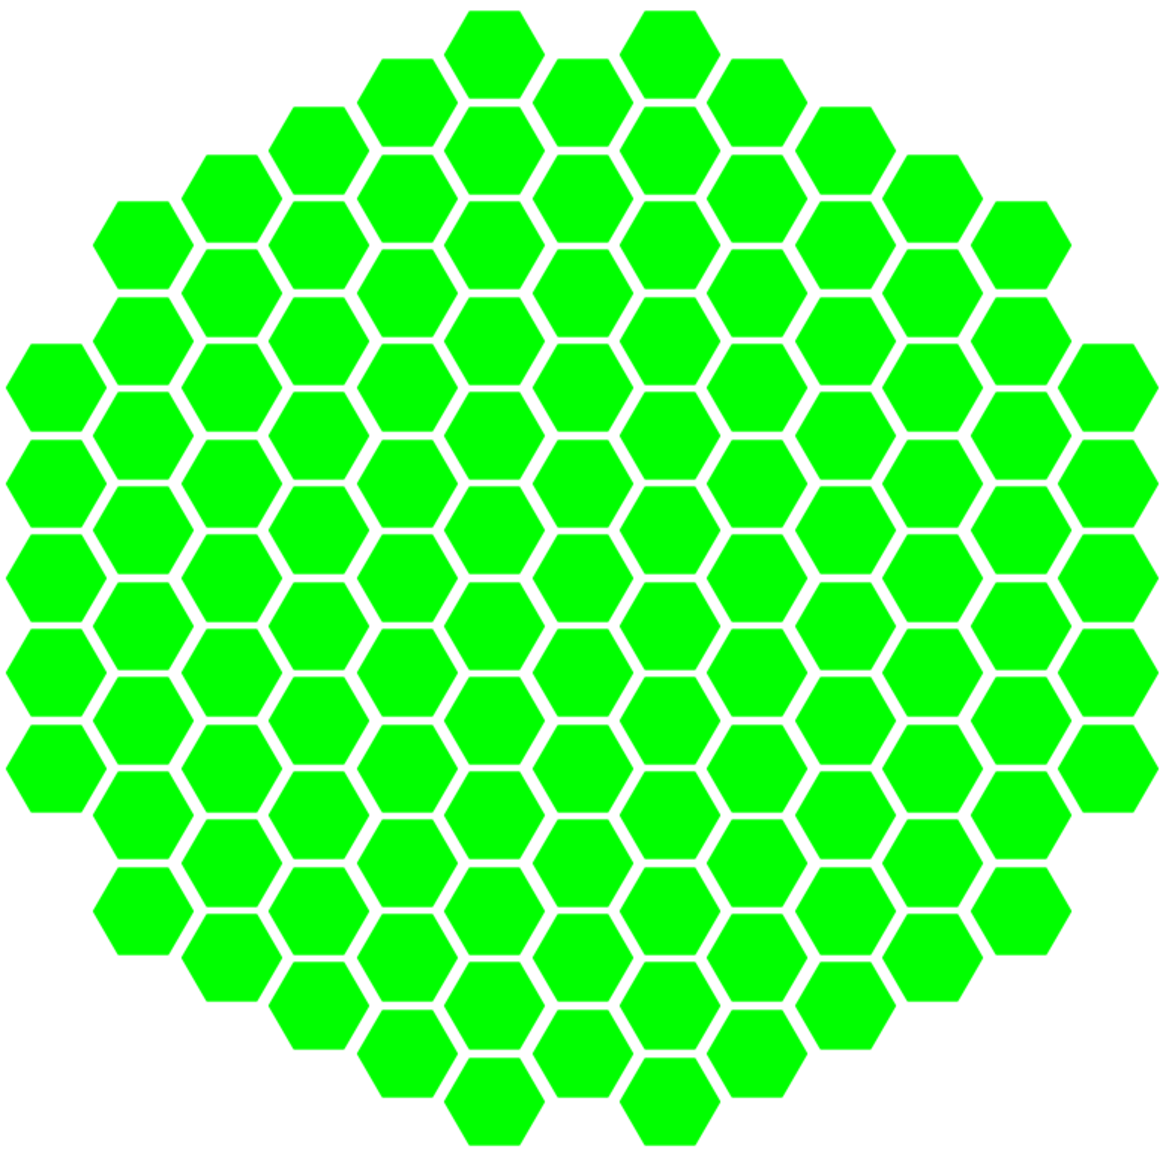
\includegraphics{Images/HCells.pdf}}}

    \only<5>{\resizebox{1.0\linewidth}{!}{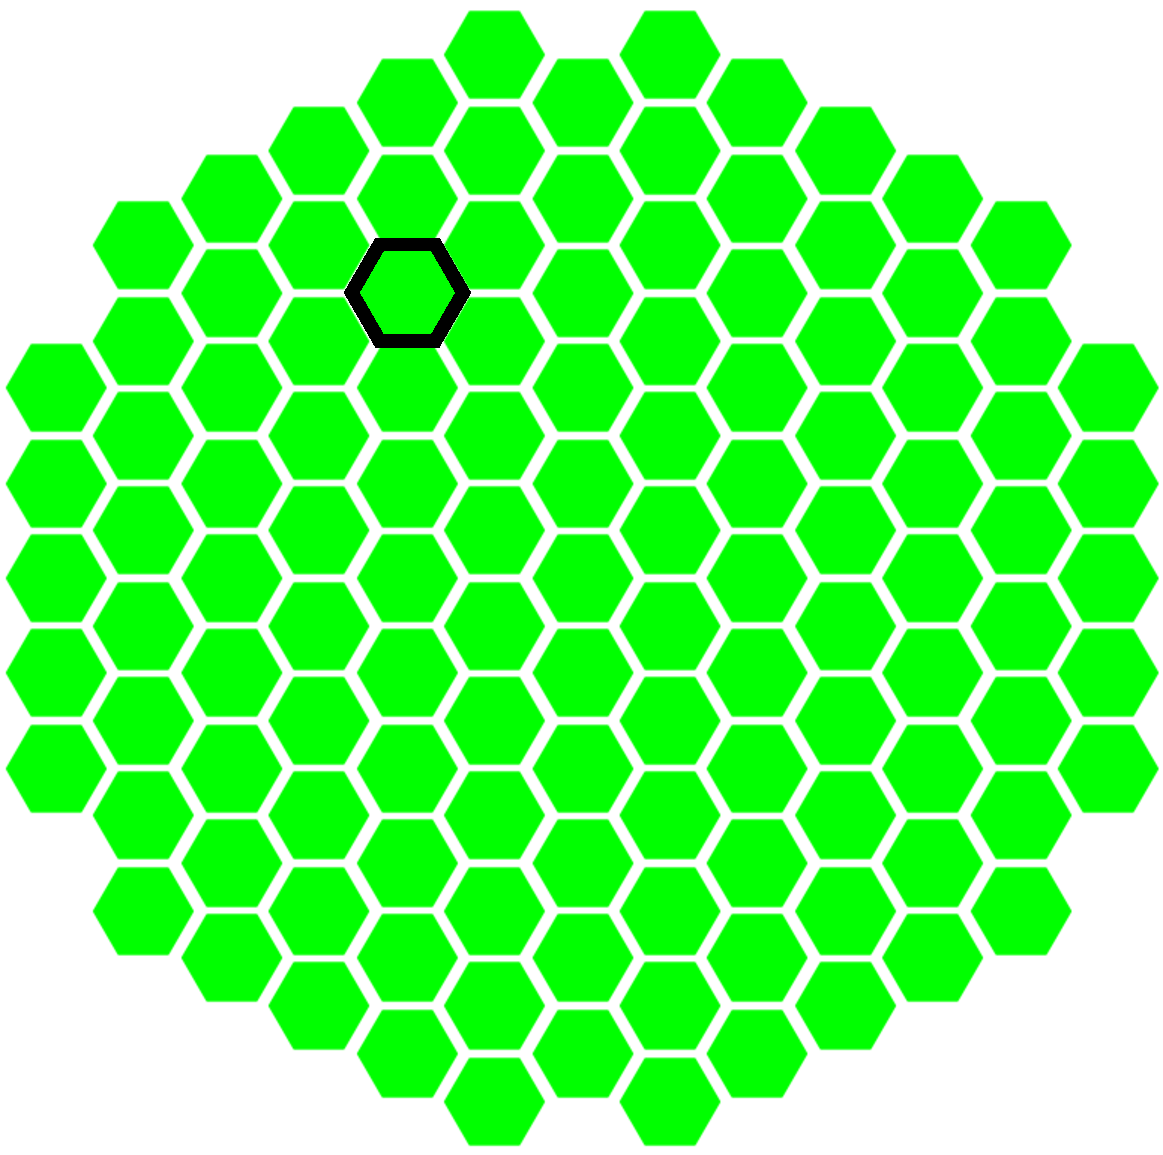
\includegraphics{Images/Freecellexample.pdf}}}

    \only<8>{\resizebox{1.0\linewidth}{!}{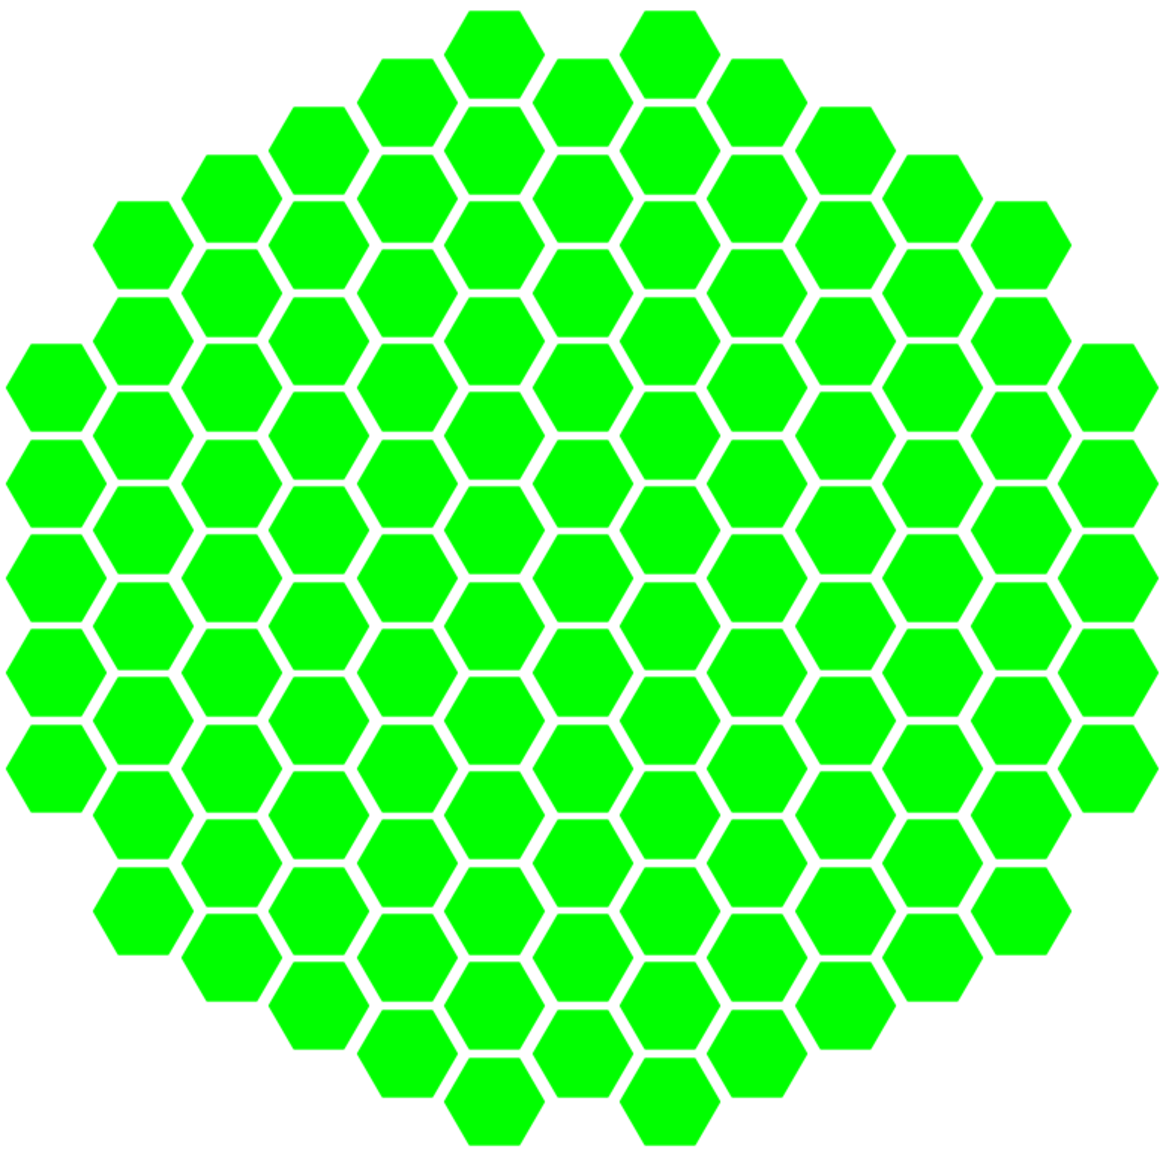
\includegraphics{Images/HCells.pdf}}}

    \only<9>{\resizebox{1.0\linewidth}{!}{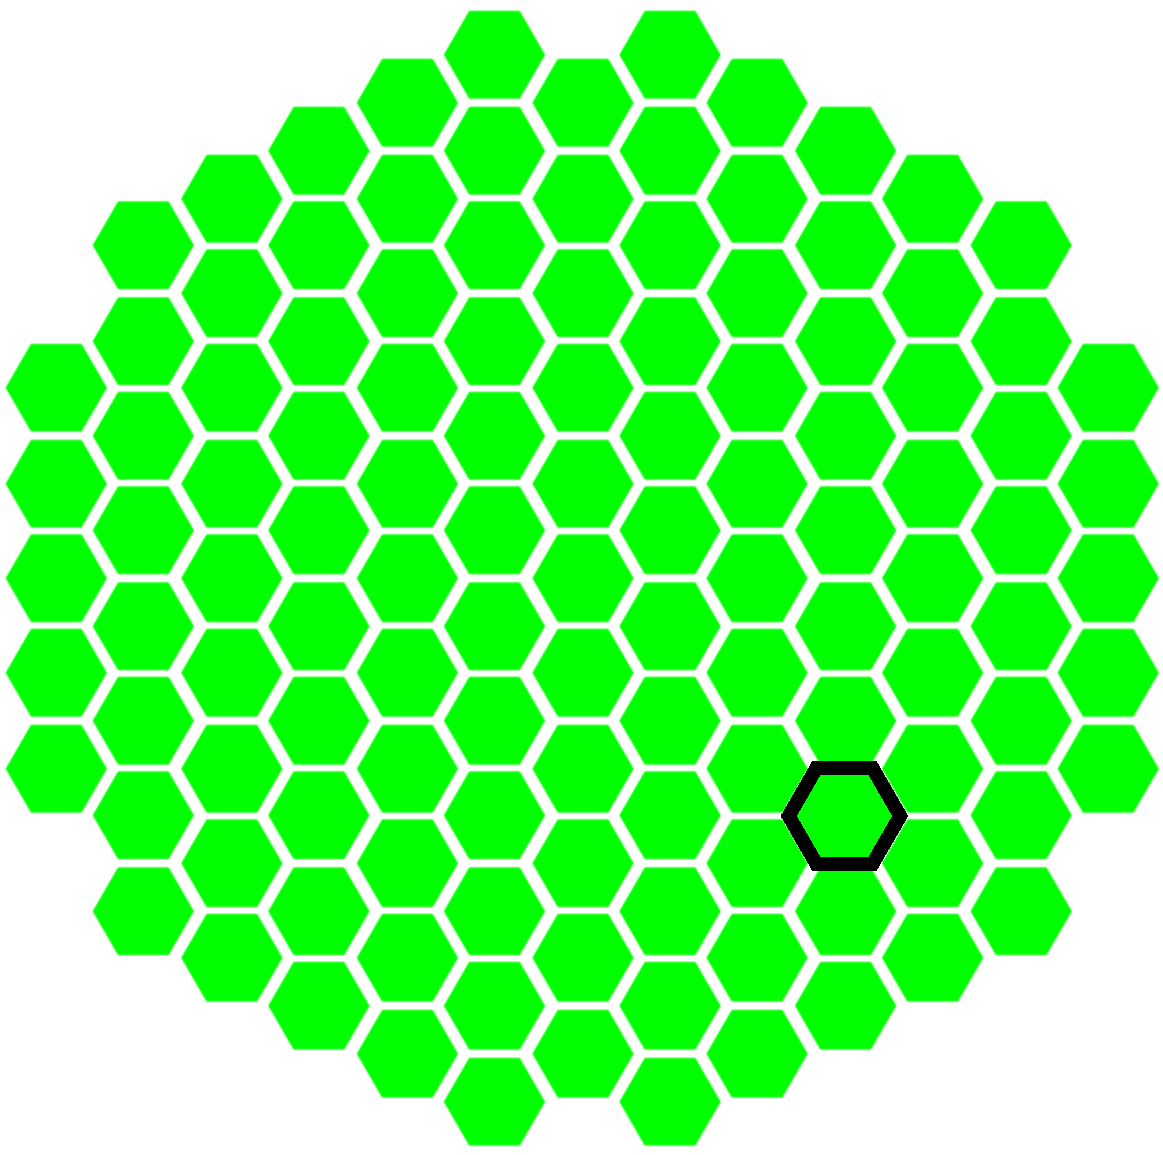
\includegraphics{Images/Cell2ellexample1.pdf}}}

    \only<10->{\resizebox{1.0\linewidth}{!}{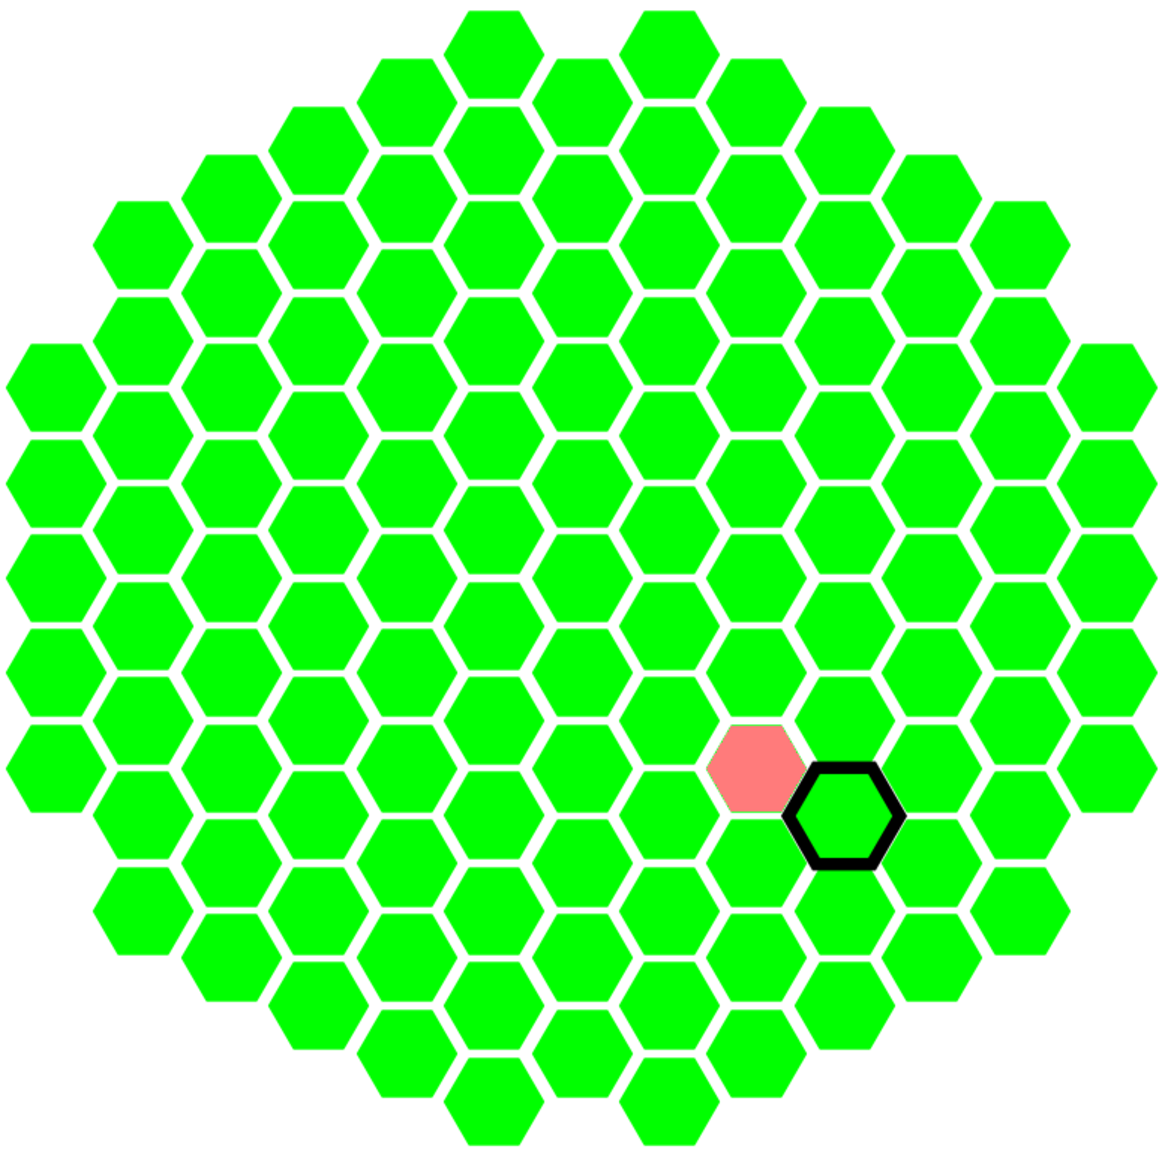
\includegraphics{Images/Cell2ellexample2.pdf}}}
    \end{center}

    \end{columns}}
    
    \vspace{0.5em}
    \onslide<11->{
    \resizebox{1.0\linewidth}{!}{\fbox{\parbox{\textwidth}{\begin{center}  
        Vary $x$ to see how different probabilities of infecting by cell to cell change the progression of an infection
    \end{center}}}}}

\end{frame}

\begin{frame}{Syncytia}

    \resizebox{1.0\linewidth}{!}{\begin{columns}
    \column{0.6\textwidth}
    \onslide<2->{Probability of Syncytia formation}
    \begin{itemize}
        \item<2-> $\mathrm{P_{s}} = \gamma$ 
            \begin{itemize}
                \item[--]<3-> $\gamma$ is a fixed number between 0 and 1
            \end{itemize}
    \end{itemize}

    \column{0.40\textwidth}
    \begin{center}
    \only<2-3>{\resizebox{1.0\linewidth}{!}{
\includegraphics{Images/Cellsblank.pdf}}}

    \only<4>{\resizebox{1.0\linewidth}{!}{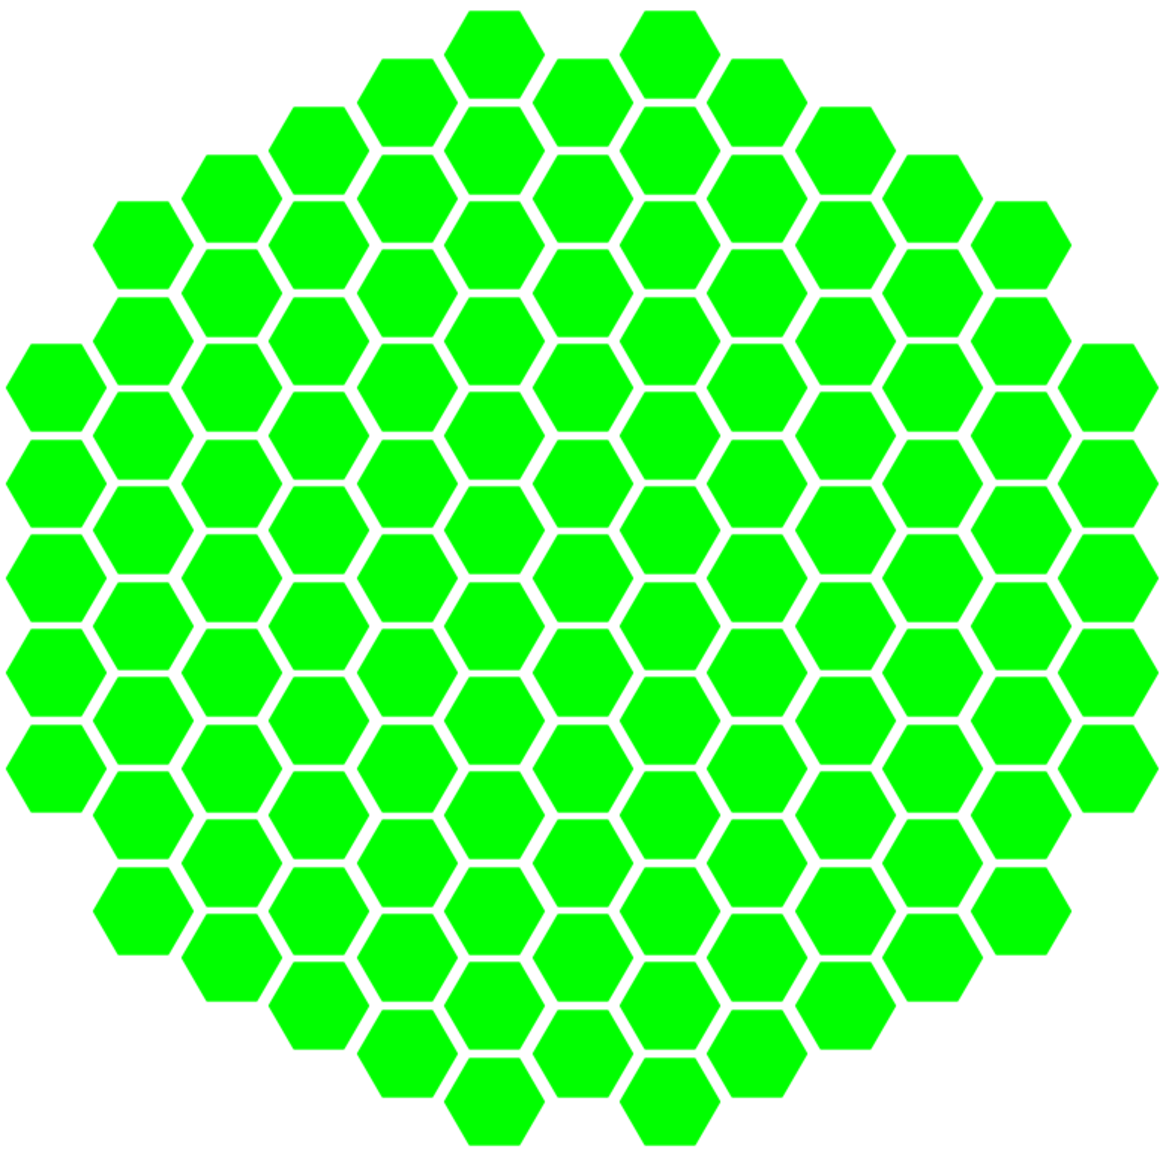
\includegraphics{Images/HCells.pdf}}}

    \only<5>{\resizebox{1.0\linewidth}{!}{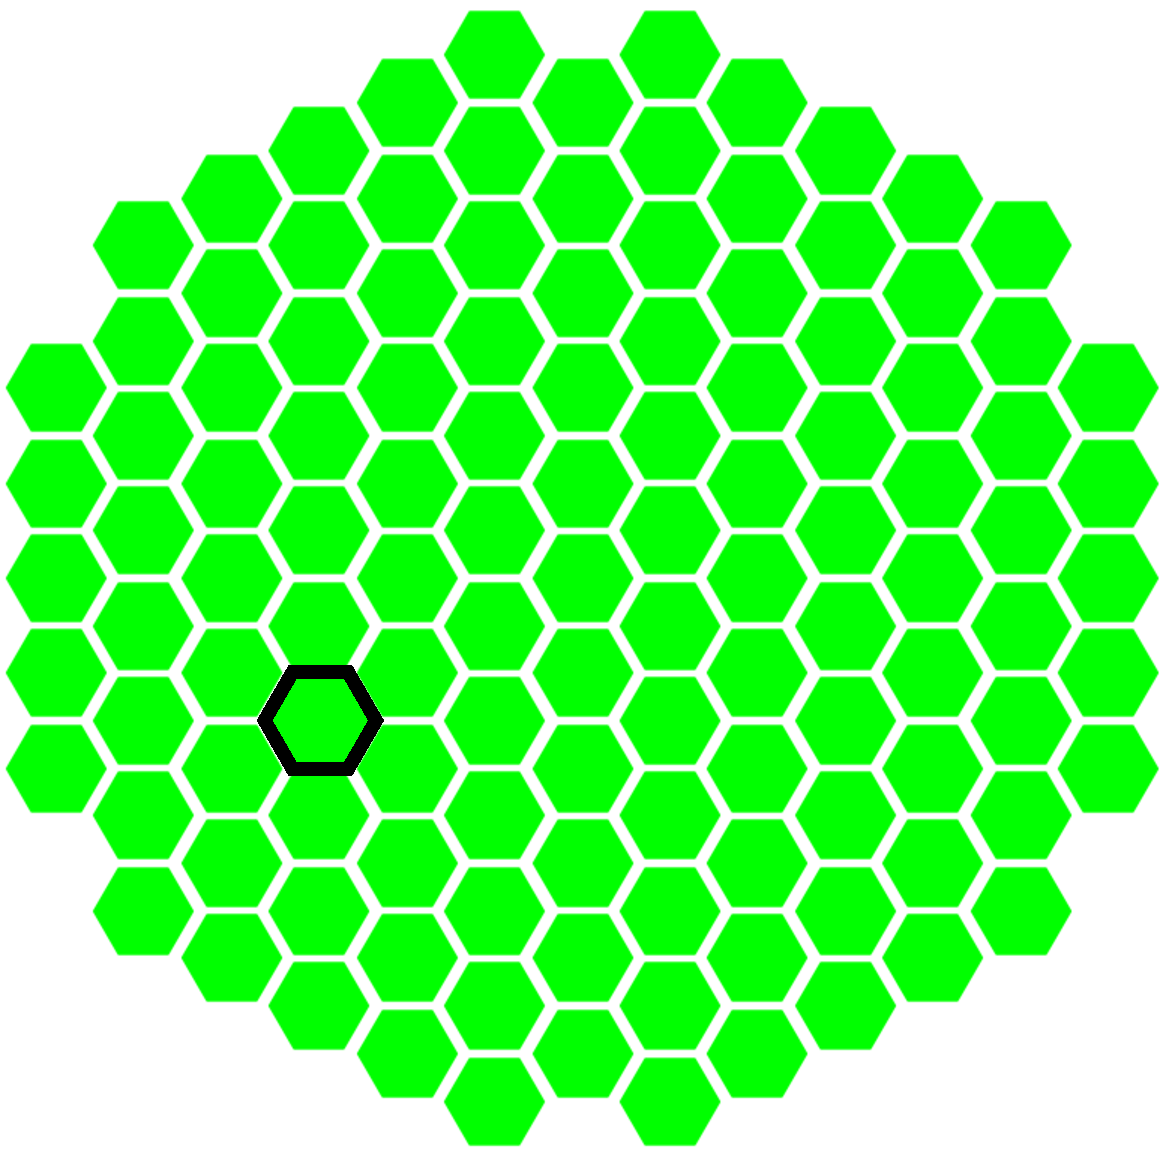
\includegraphics{Images/Syncytiaexample1.pdf}}}

    \only<6->{\resizebox{1.0\linewidth}{!}{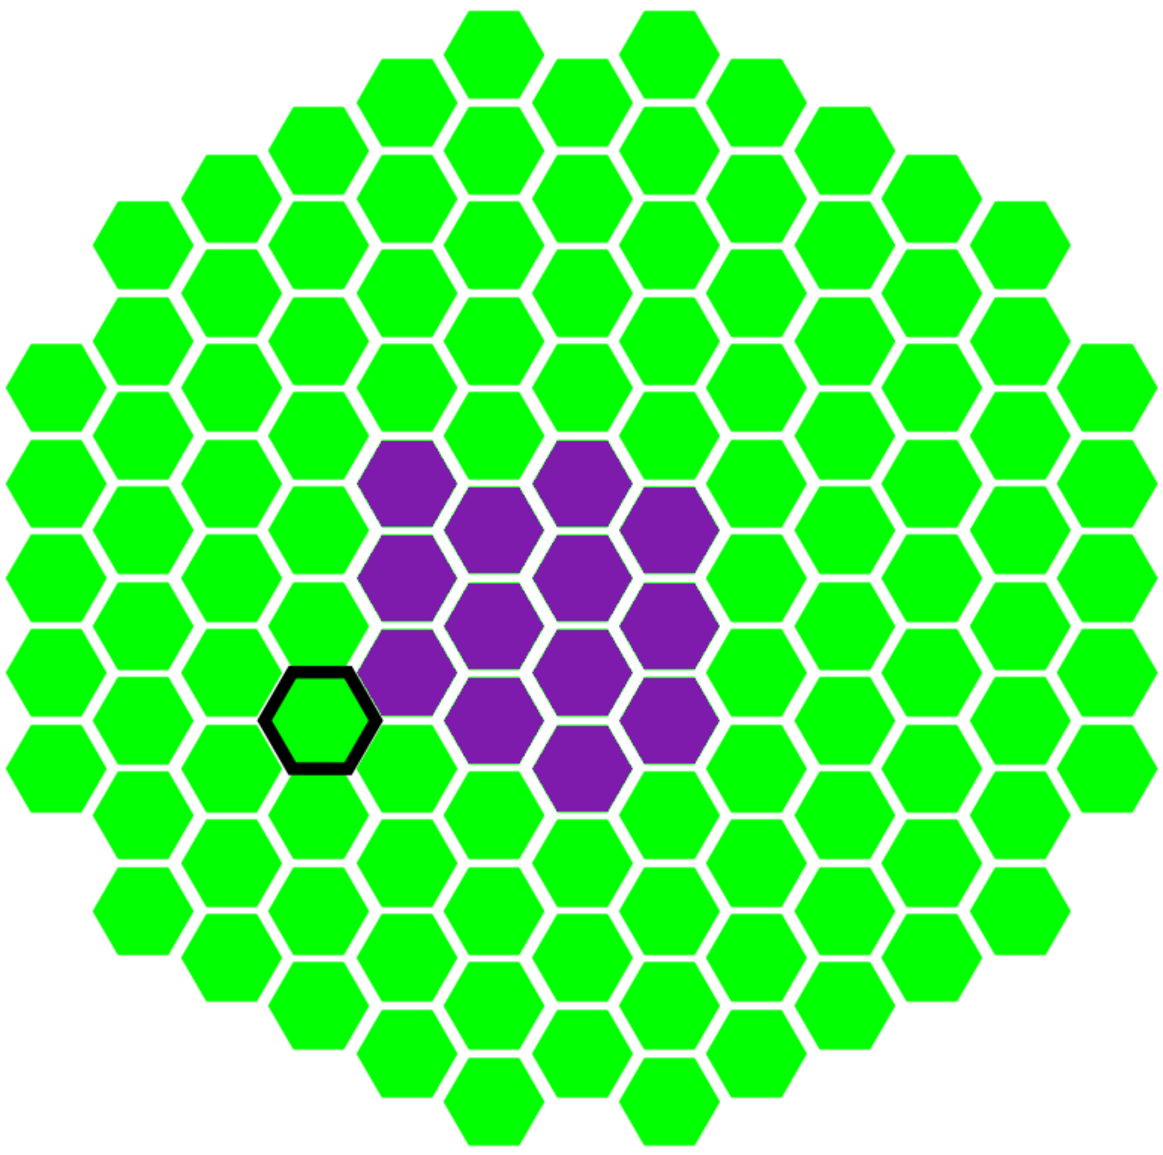
\includegraphics{Images/Syncytiaexample2.pdf}}}
    \end{center}

    \end{columns}}
    
    \vspace{0.5em}
    \onslide<7->{
    \resizebox{1.0\linewidth}{!}{\fbox{\parbox{\textwidth}{\begin{center}  
        Vary $\gamma$ to see how different probabilities of syncytia formation change the progression of an infection
    \end{center}}}}}    

\end{frame}

% Syntax: \colorboxed[<color model>]{<color specification>}{<math formula>}
\newcommand*{\colorboxed}{}
\def\colorboxed#1#{%
  \colorboxedAux{#1}%
}
\newcommand*{\colorboxedAux}[3]{%
  % #1: optional argument for color model
  % #2: color specification
  % #3: formula
  \begingroup
    \colorlet{cb@saved}{.}%
    \color#1{#2}%
    \boxed{%
      \color{cb@saved}%
      #3%
    }%
  \endgroup
}

\begin{frame}{Advection}

    \resizebox{1.0\linewidth}{!}{\begin{columns}
    \column{0.65\textwidth}
    \onslide<2->{Motion of Virus}
    \begin{itemize}
        \item<2-> $\colorboxed{white}{\frac{\partial V}{\partial t}} = D\nabla^{2}V + pI - cV \onslide<3->{+} \onslide<3->{\colorboxed{red}{\mu \frac{\partial V}{\partial z}}}$
            \begin{itemize}
                \item[--]<4-> $V$ is the amount of virus that is above a cell
                \item[--]<4-> $D$ is the diffusion matrix
                \item[--]<4-> $p$ is the production rate
                \item[--]<4-> $c$ is the clearance rate
                \item[--]<4-> $\mu$ is the speed of the mucus
            \end{itemize}
    \end{itemize}

    \column{0.40\textwidth}
    \onslide<5->{
    \begin{center}
        \resizebox{1.0\linewidth}{!}{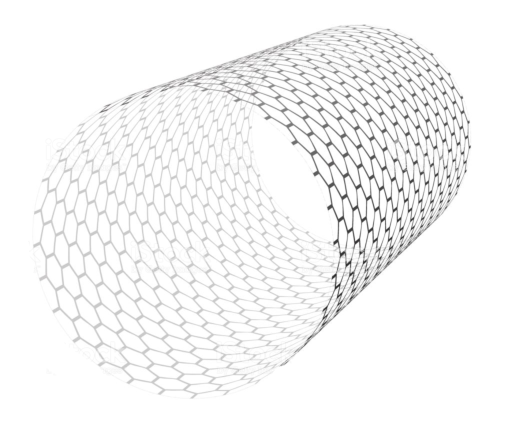
\includegraphics{Images/Hexagonal_Mesh_Pipe.pdf}}
    \end{center}}

    \end{columns}}
    
    \vspace{0.5em}
    \onslide<6->{
    \resizebox{1.0\linewidth}{!}{\fbox{\parbox{\textwidth}{\begin{center}  
        Vary $\mu$ to see how different mucus speeds change the progression of an infection and to see if a critical speed of advection can be found
    \end{center}}}}}

\end{frame}

\begin{frame}{What will be measured}

    \begin{center}
    \only<5>{\resizebox{1.0\linewidth}{!}{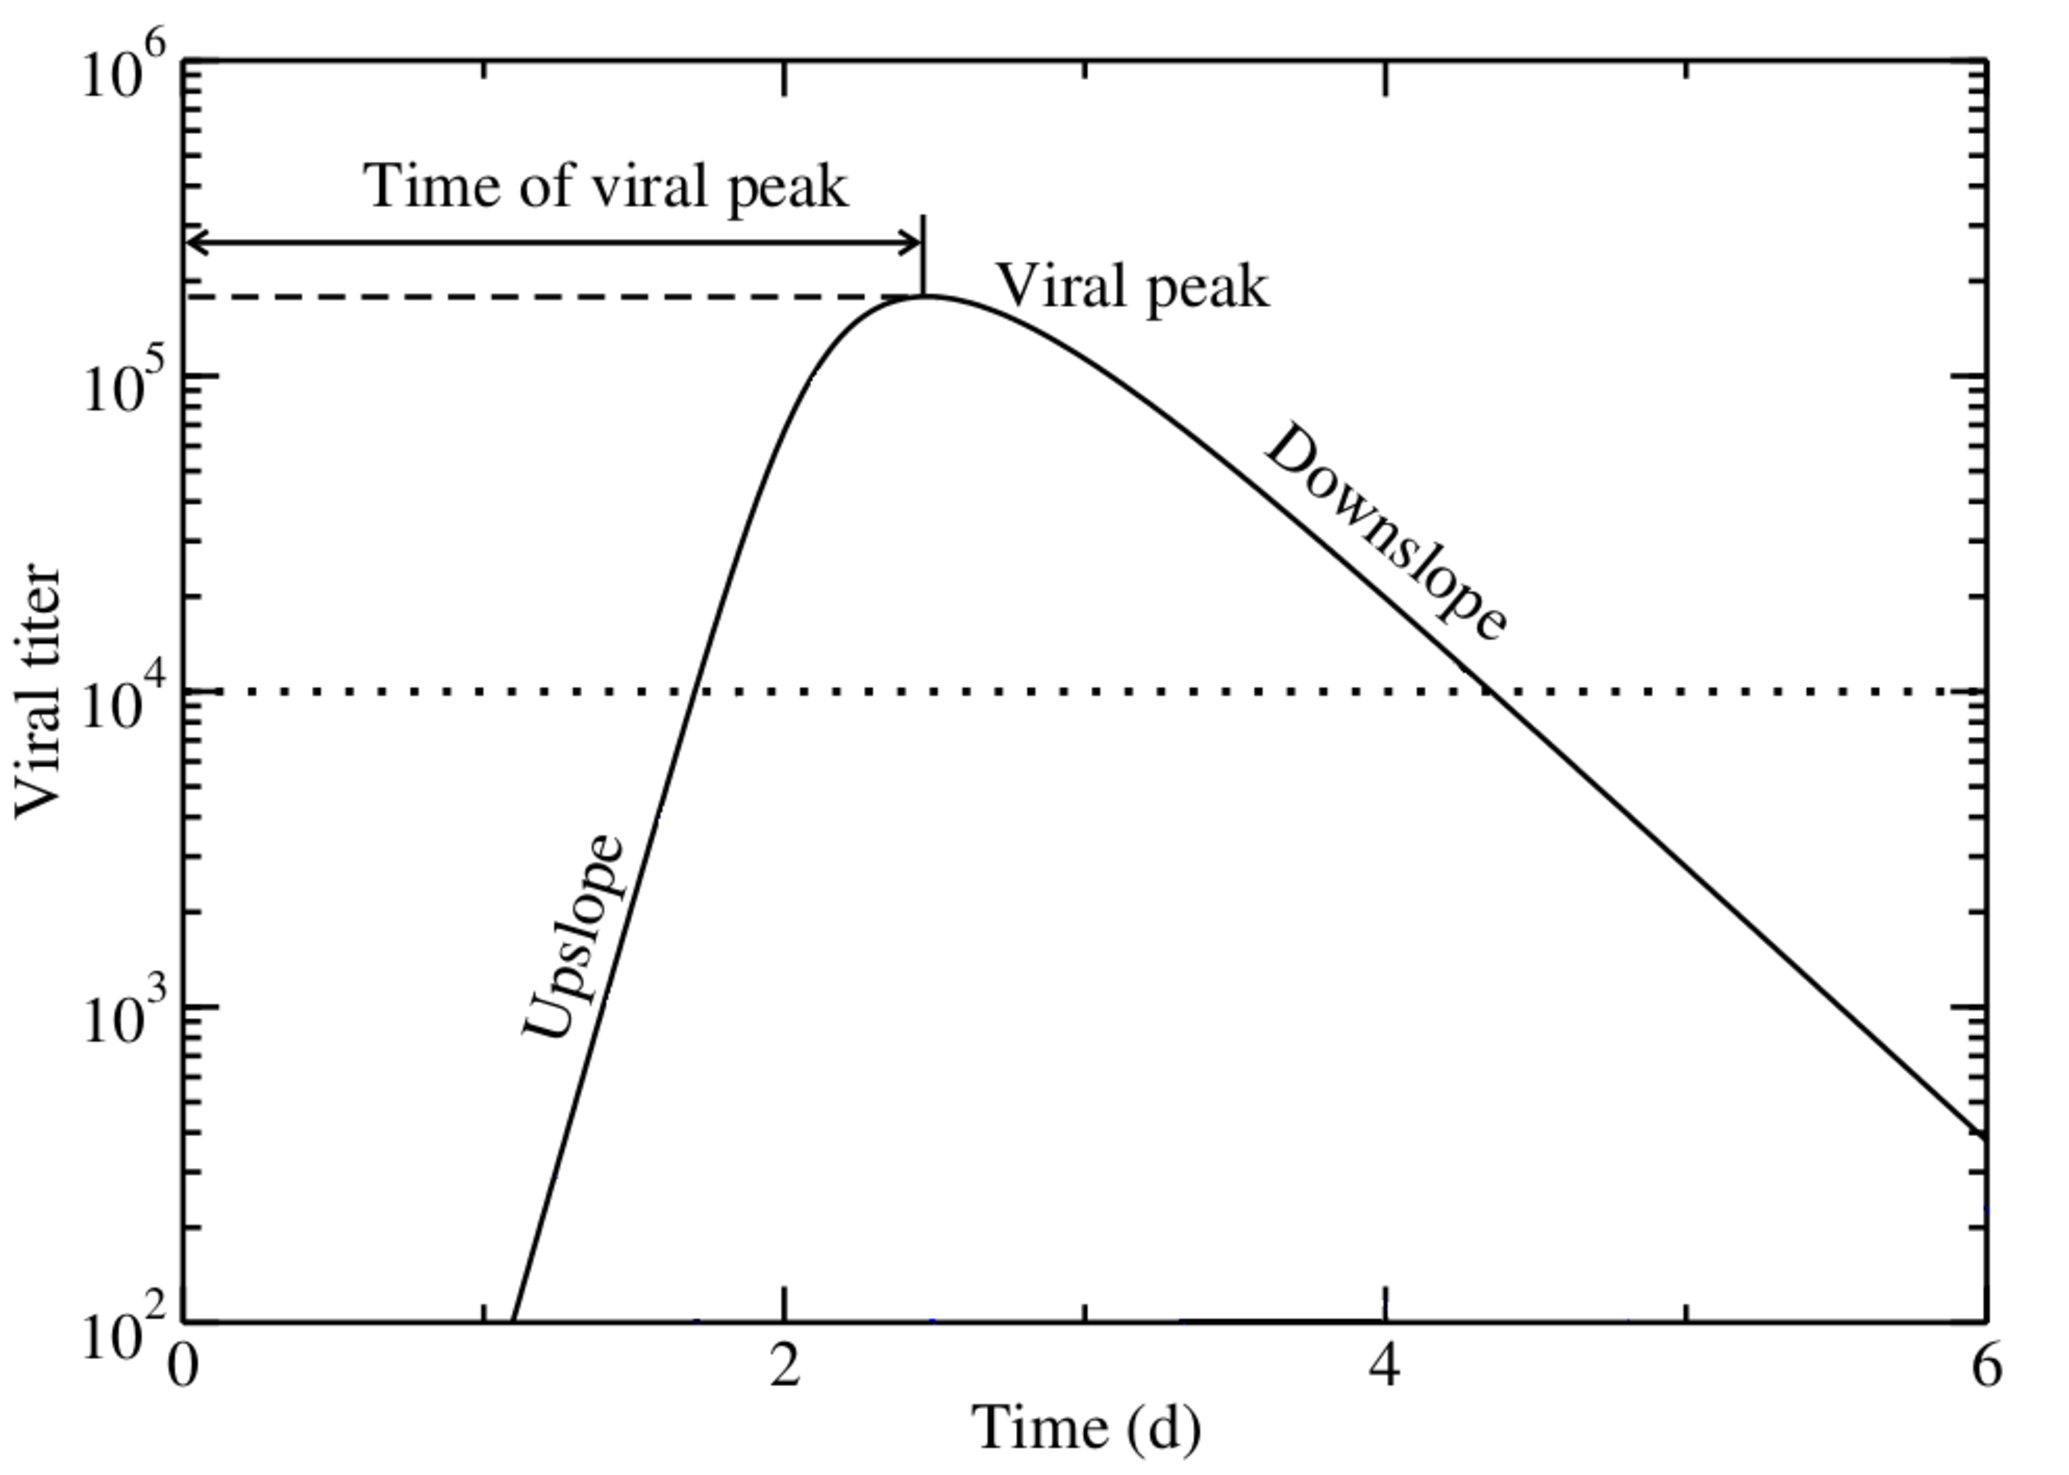
\includegraphics{Images/Measurements/Measurements.pdf}}}
    \only<1>{\resizebox{1.0\linewidth}{!}{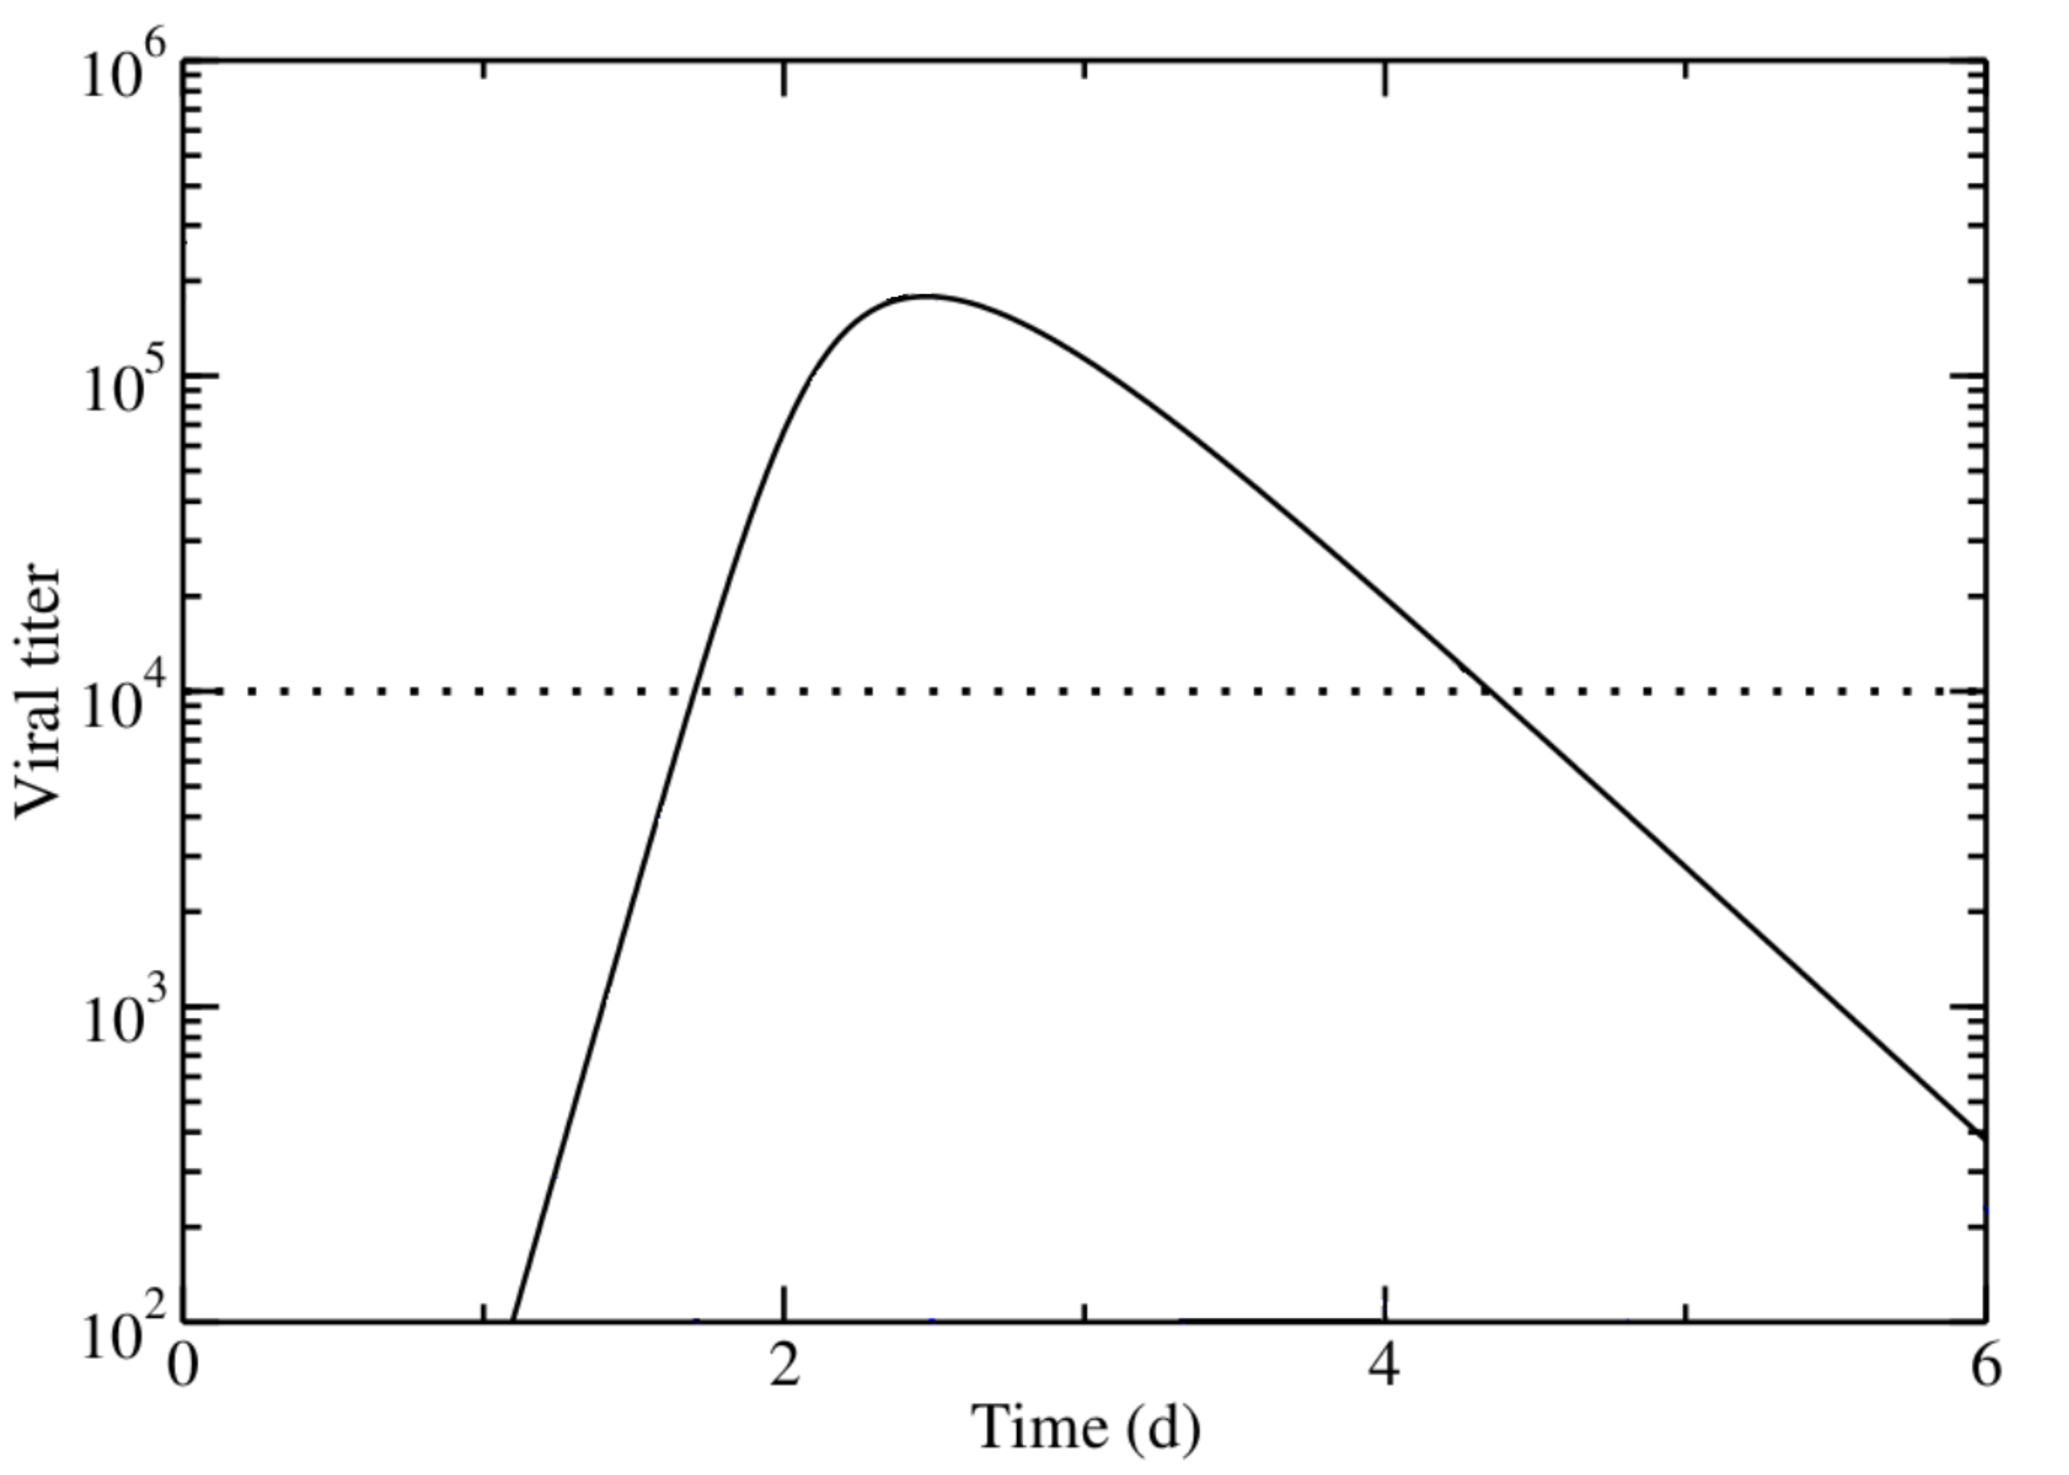
\includegraphics{Images/Measurements/Measurements1.pdf}}}
    \only<2>{\resizebox{1.0\linewidth}{!}{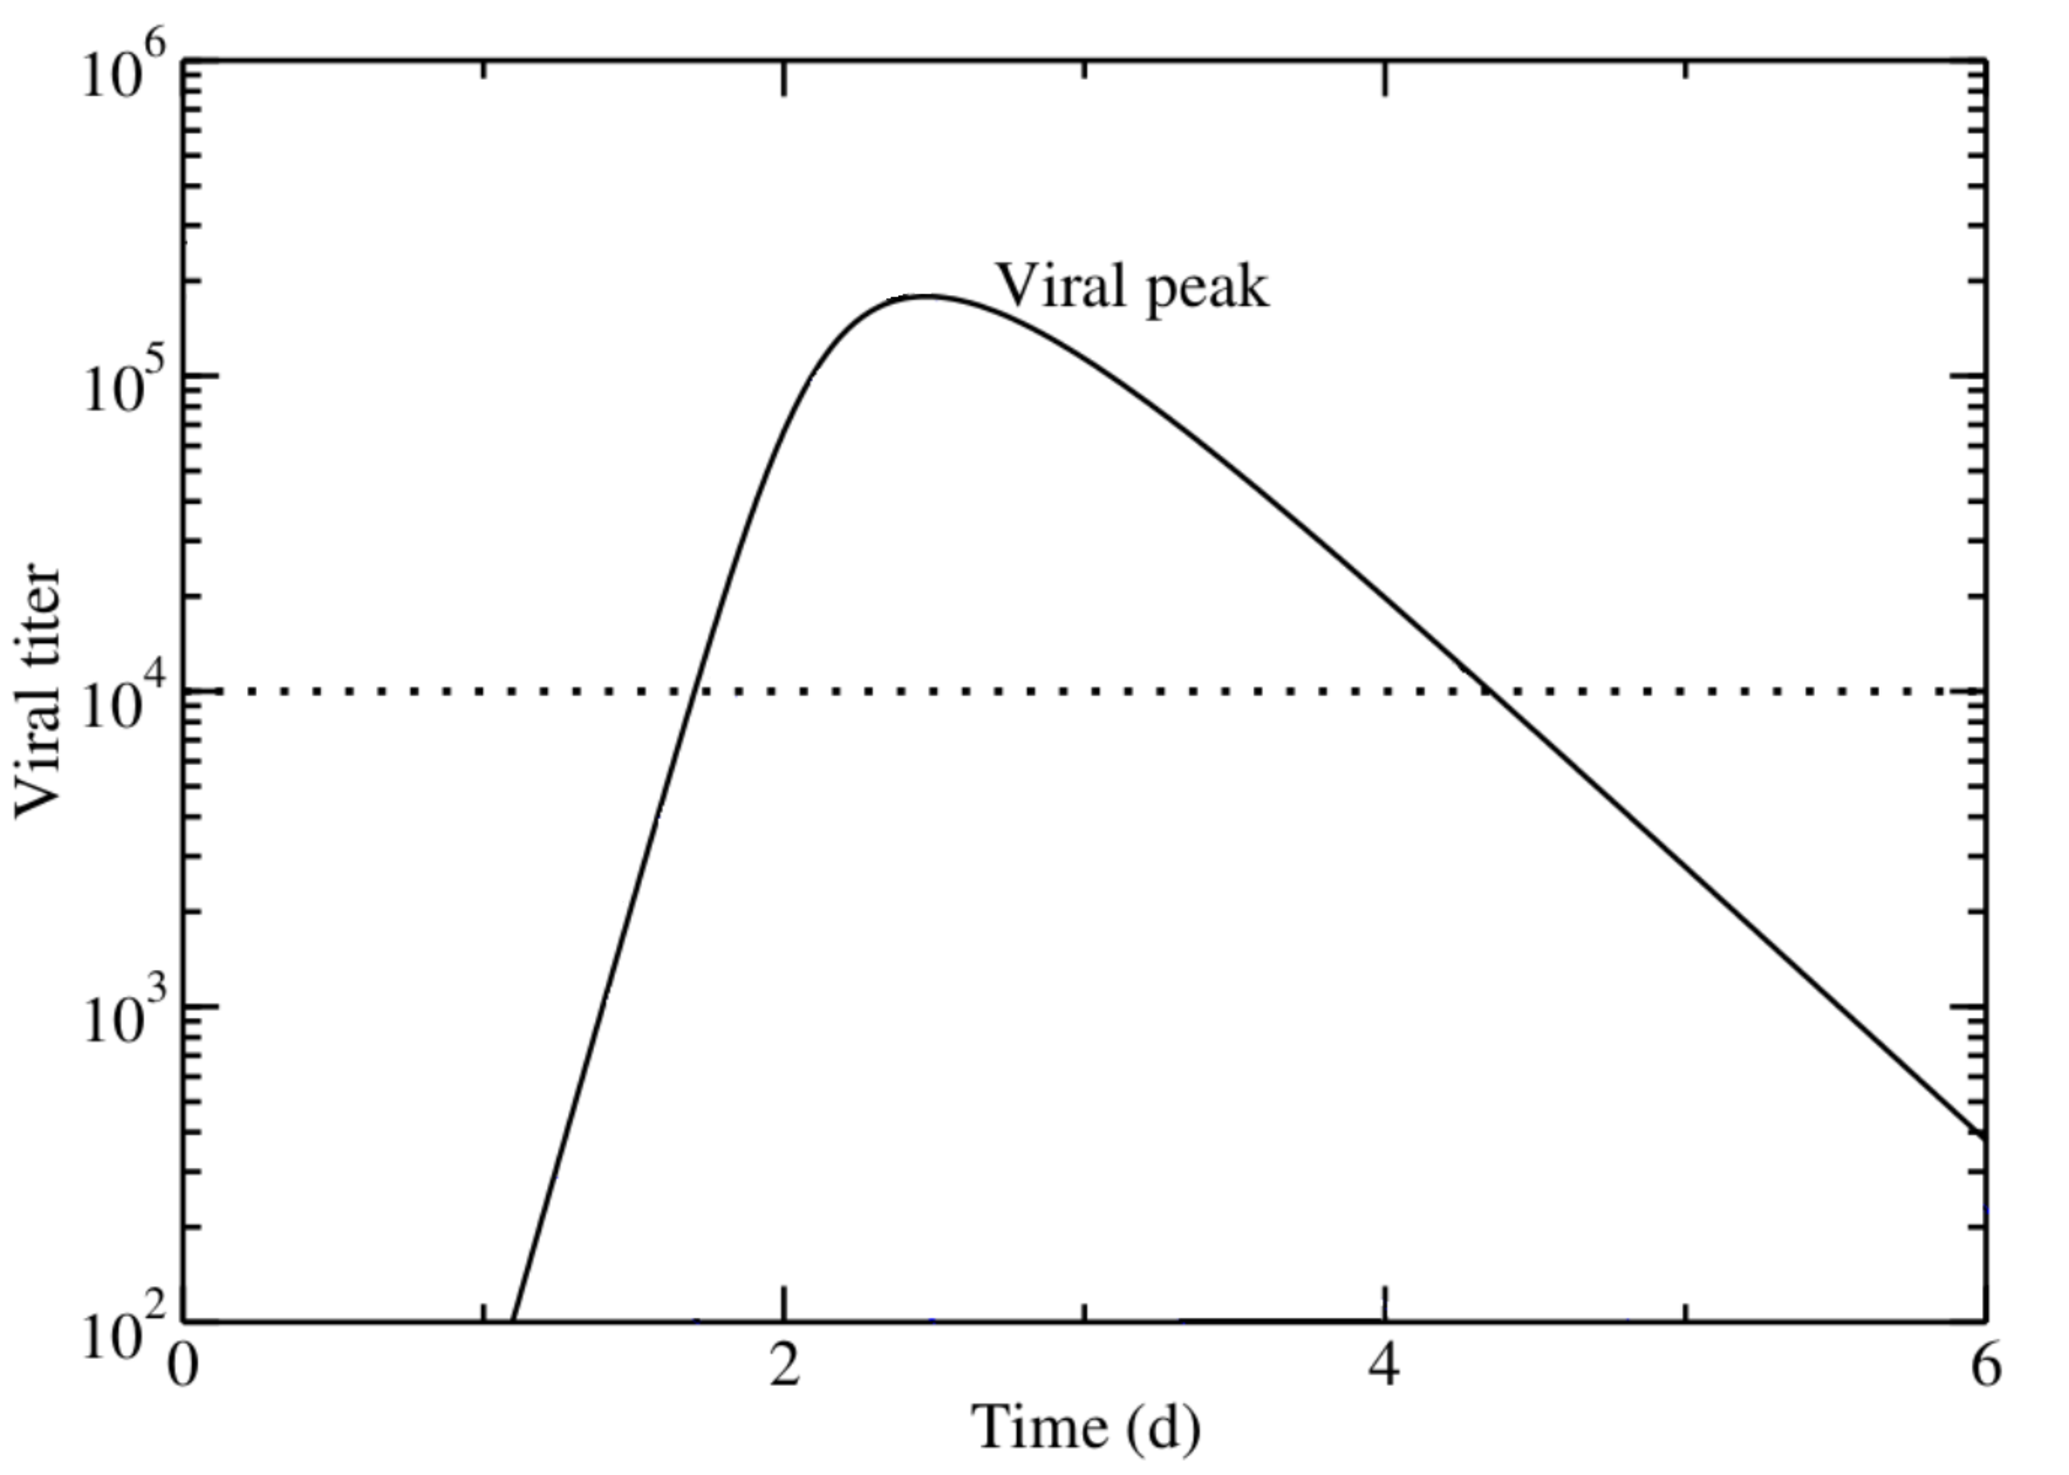
\includegraphics{Images/Measurements/Measurements2.pdf}}}
    \only<3>{\resizebox{1.0\linewidth}{!}{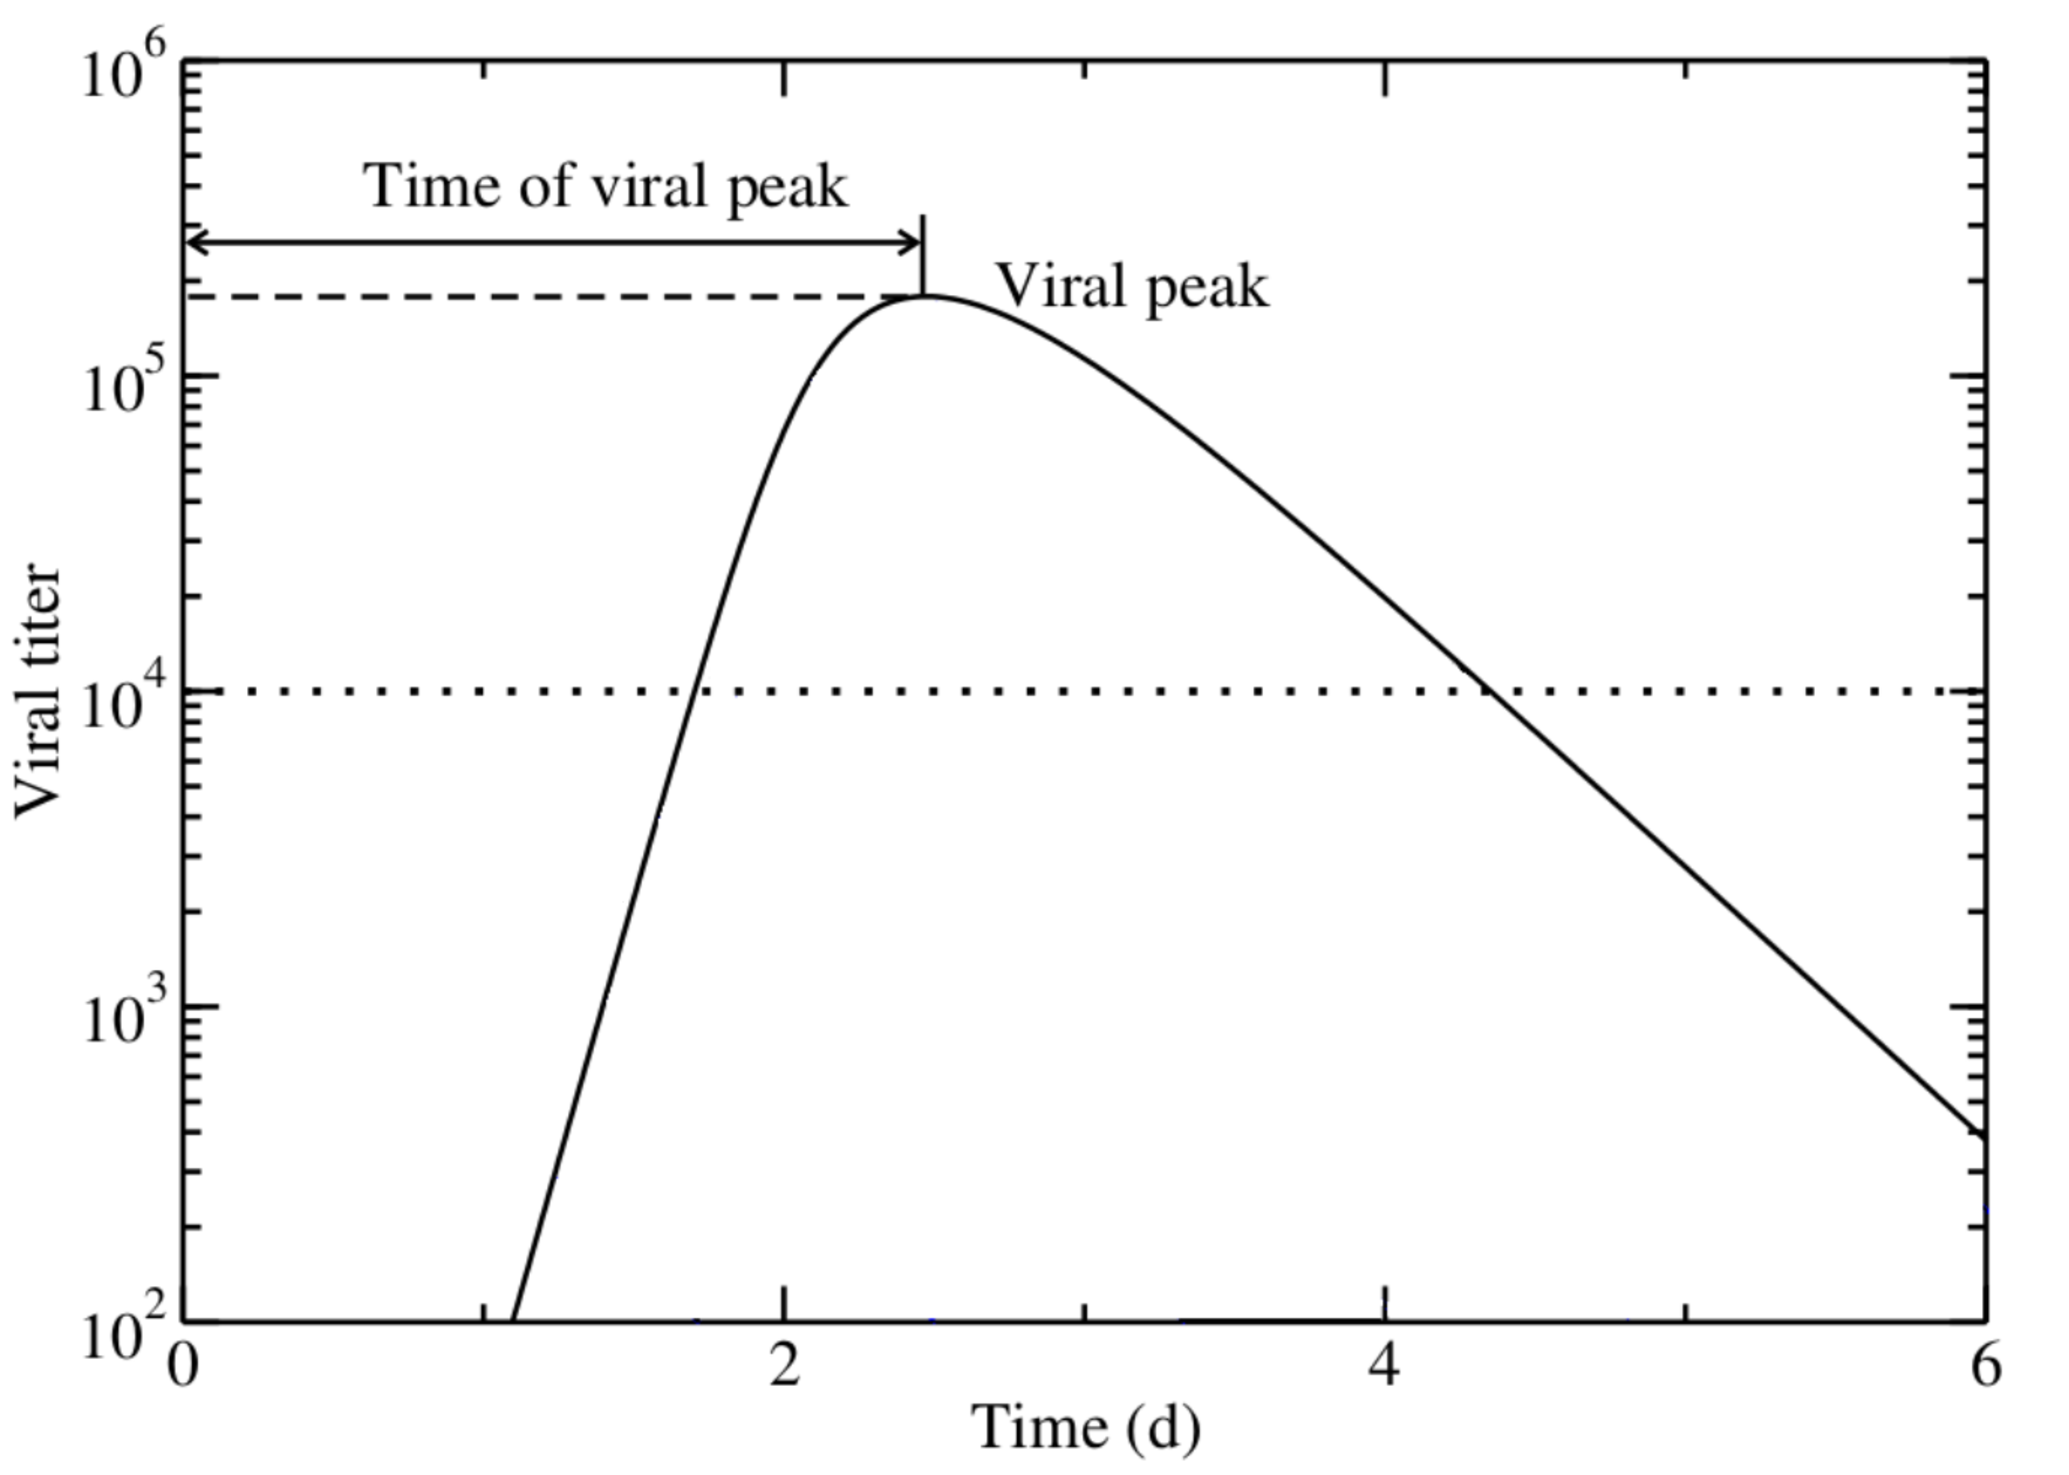
\includegraphics{Images/Measurements/Measurements3.pdf}}}
    \only<4>{\resizebox{1.0\linewidth}{!}{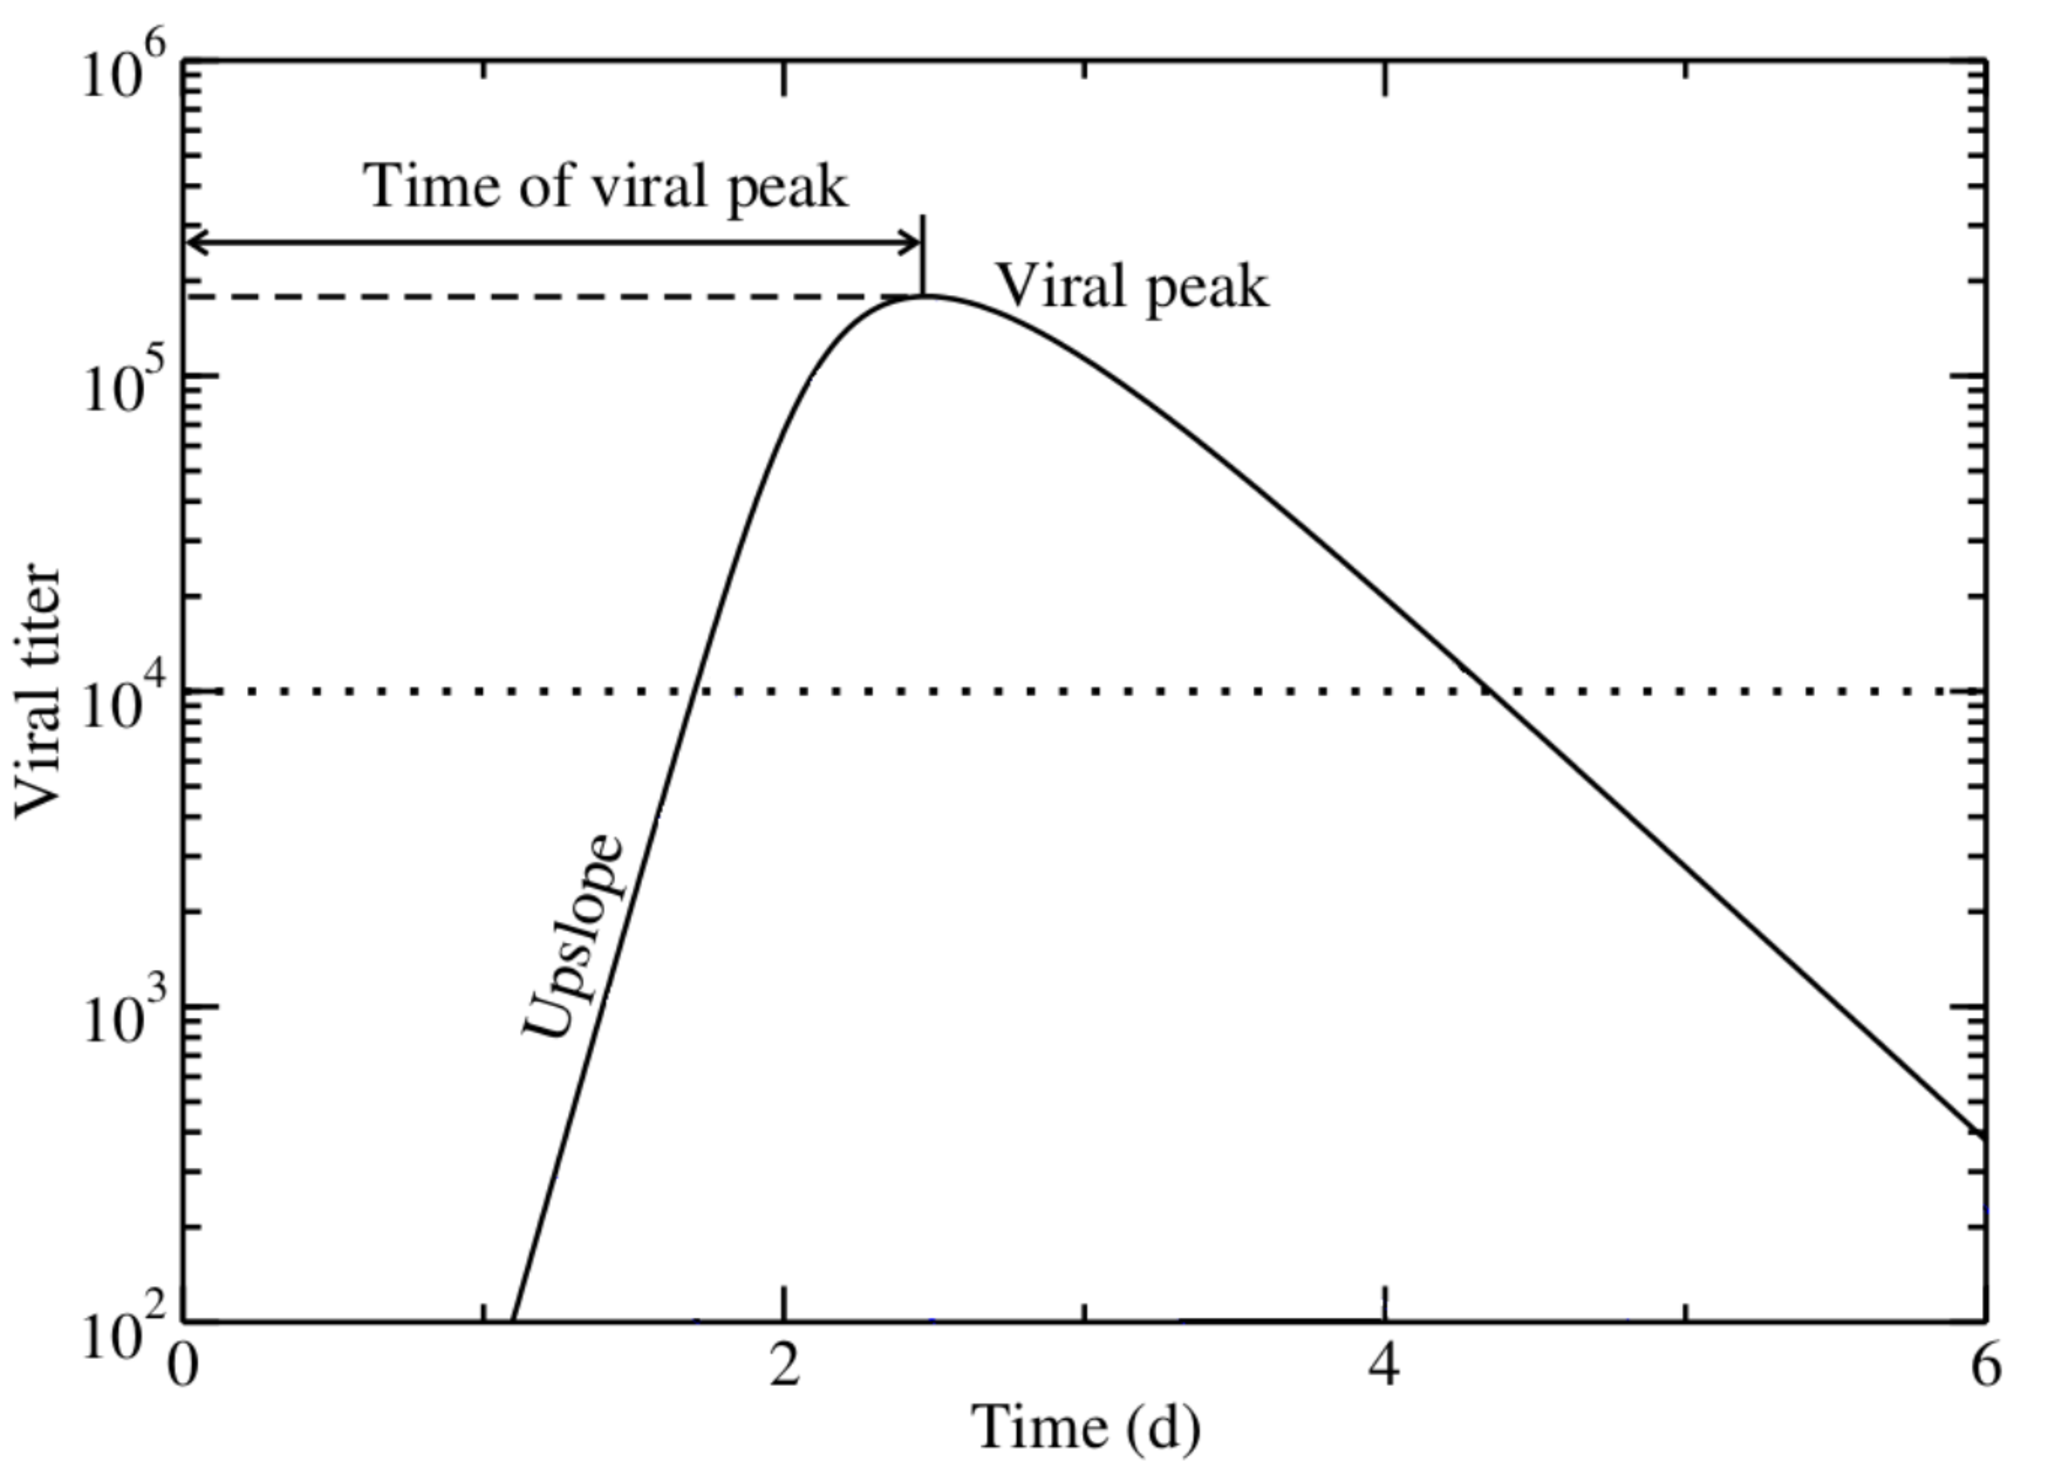
\includegraphics{Images/Measurements/Measurements4.pdf}}}
    \end{center}

\end{frame}

%-----------------------------------------------------------------------------------
\section{Work to date/Timeline}

\begin{frame}{Simulations}

    \resizebox{1.0\linewidth}{!}{\begin{columns}[T]
    \column{0.5\textwidth}
    \begin{center}
    Cell to cell
    \end{center}

    \column{0.5\textwidth}
    \begin{center}
    Cell free
    \end{center}    

    \end{columns}}

    \hspace{-0.26cm}
    \resizebox{1.0\linewidth}{!}{\begin{columns}[T]
    \column{0.5\textwidth}
    \begin{center}
    \only<2->{\resizebox{1.0\textwidth}{!}{\animategraphics[autoplay]{20}{Cell2cell/cell}{0}{199}}}
    \only<1>{\resizebox{1.0\linewidth}{!}{
\includegraphics{Cell2cell/cell0.png}}}
    \end{center}

    \column{0.5\textwidth}
    \begin{center}
    \only<2->{\resizebox{1.0\textwidth}{!}{\animategraphics[autoplay]{20}{Cellfree/cell}{0}{199}}}
    \only<1>{\resizebox{1.0\linewidth}{!}{
\includegraphics{Cellfree/cell0.png}}}
    \end{center}    

    \end{columns}}

\end{frame}

\begin{frame}{Measurements}

    \begin{itemize}
        \item<2-> Different initial amounts of virus
            \begin{itemize}
                \item[--]<3-> Health workers getting severe form of infection
            \end{itemize}
        \item<4-> Represented by the multiplicity of infection (MOI)
            \begin{itemize}
                \item[--]<5-> MOI is the ratio of the number of viruses to target cells
            \end{itemize}
    \end{itemize}

    \begin{center}
    \onslide<6->{\resizebox{1.0\linewidth}{!}{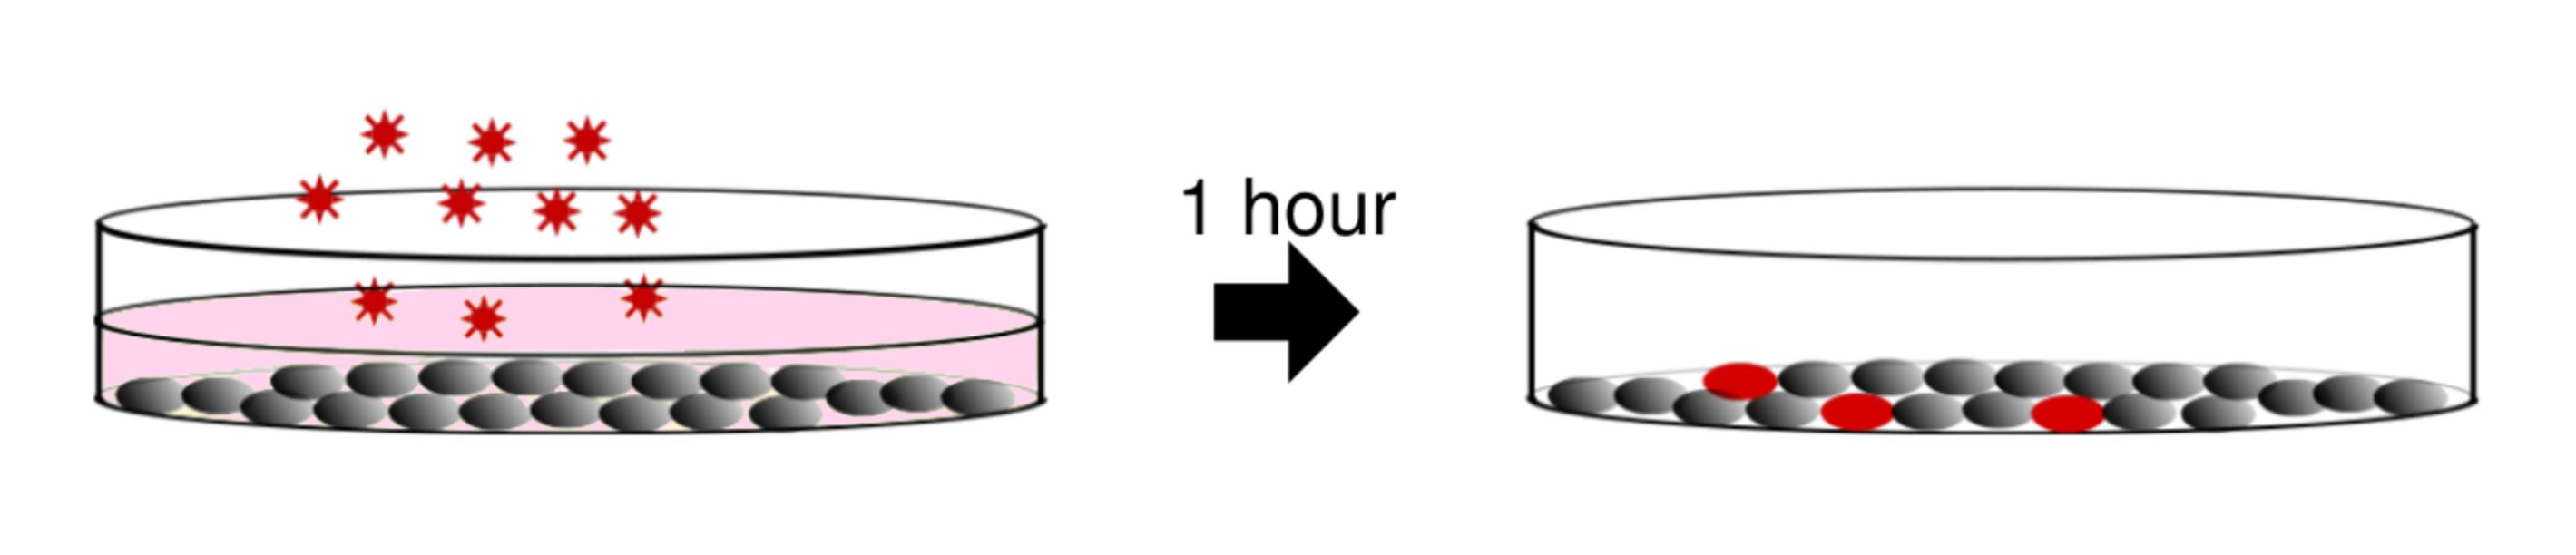
\includegraphics{Images/measurements-slide.pdf}}}
    \end{center}

\end{frame}

\begin{frame}{Results}

    \begin{center}
    \onslide<2->{\resizebox{0.4\linewidth}{!}{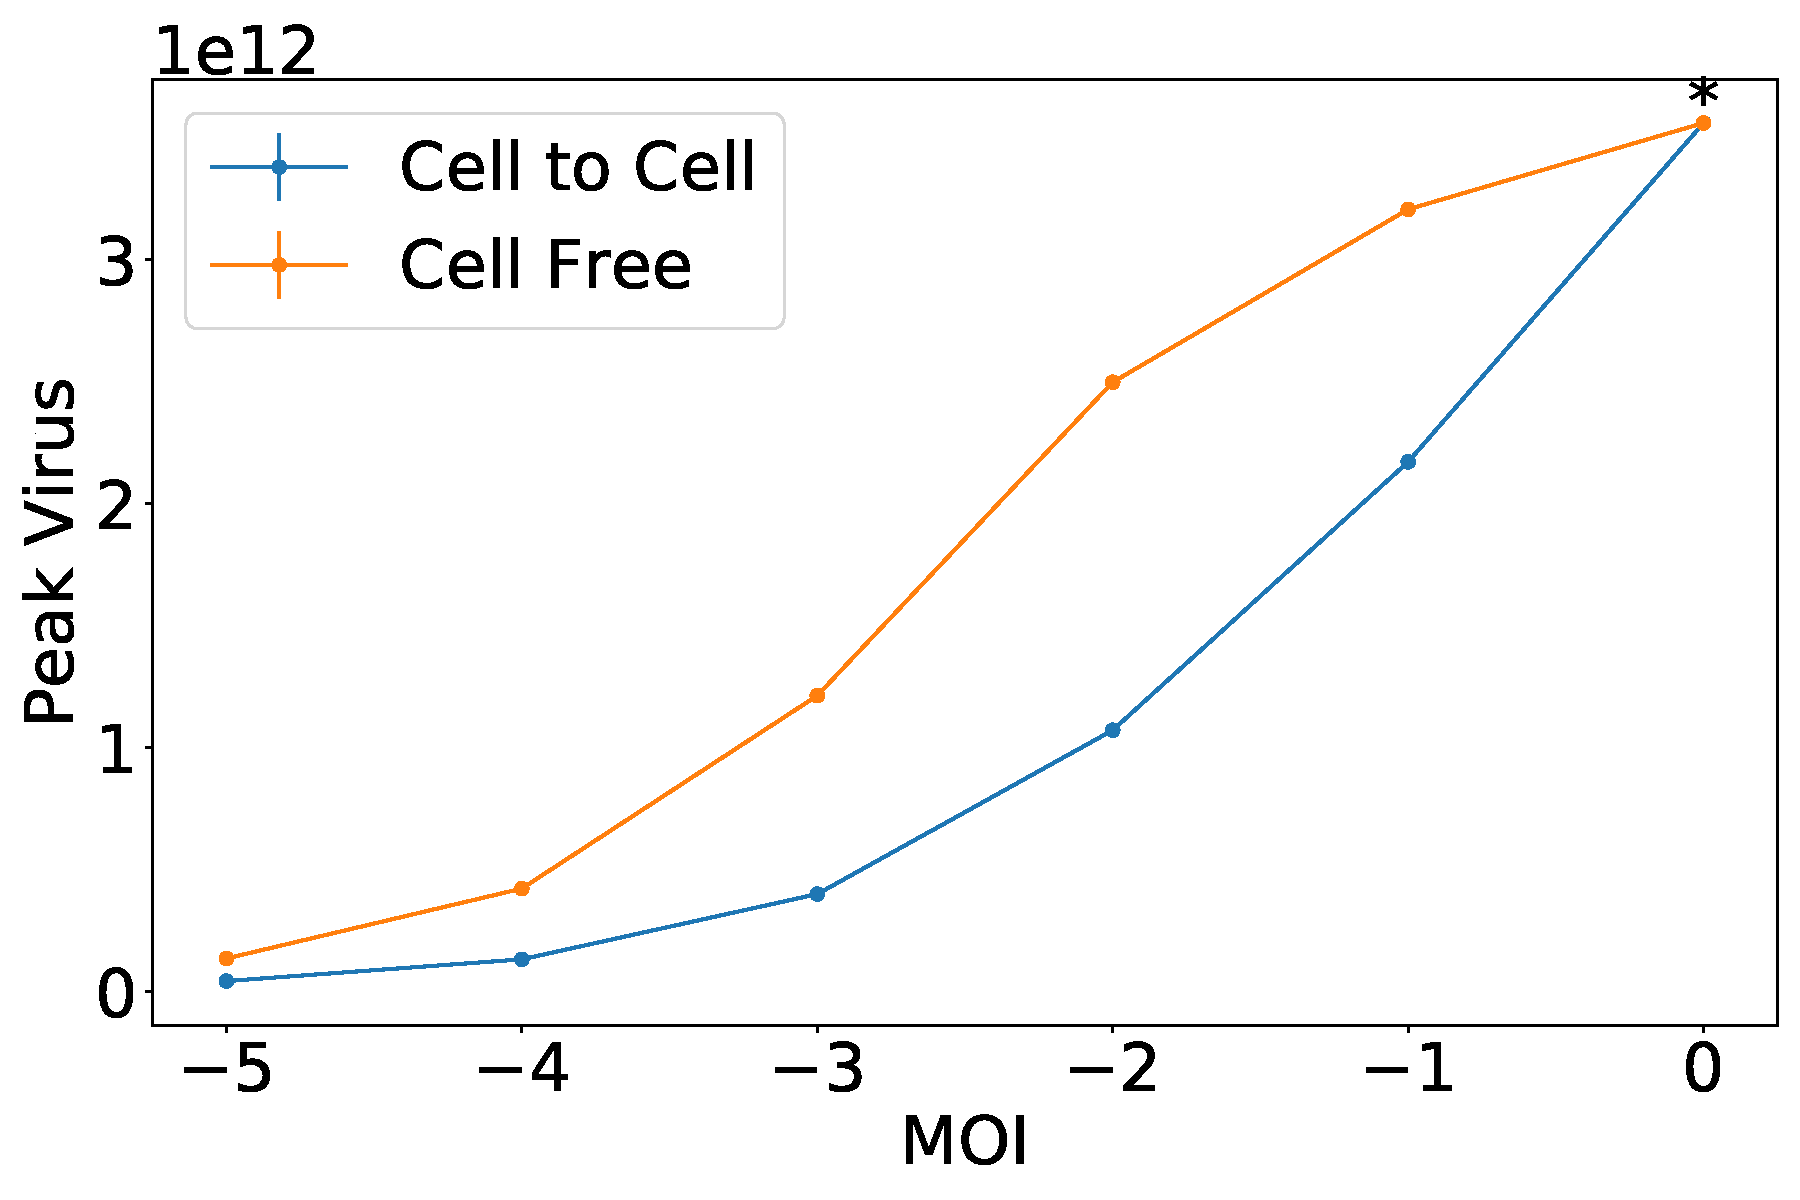
\includegraphics{Graphs/PeakViralTittervsMOI.pdf}}}
    \onslide<3->{\resizebox{0.4\linewidth}{!}{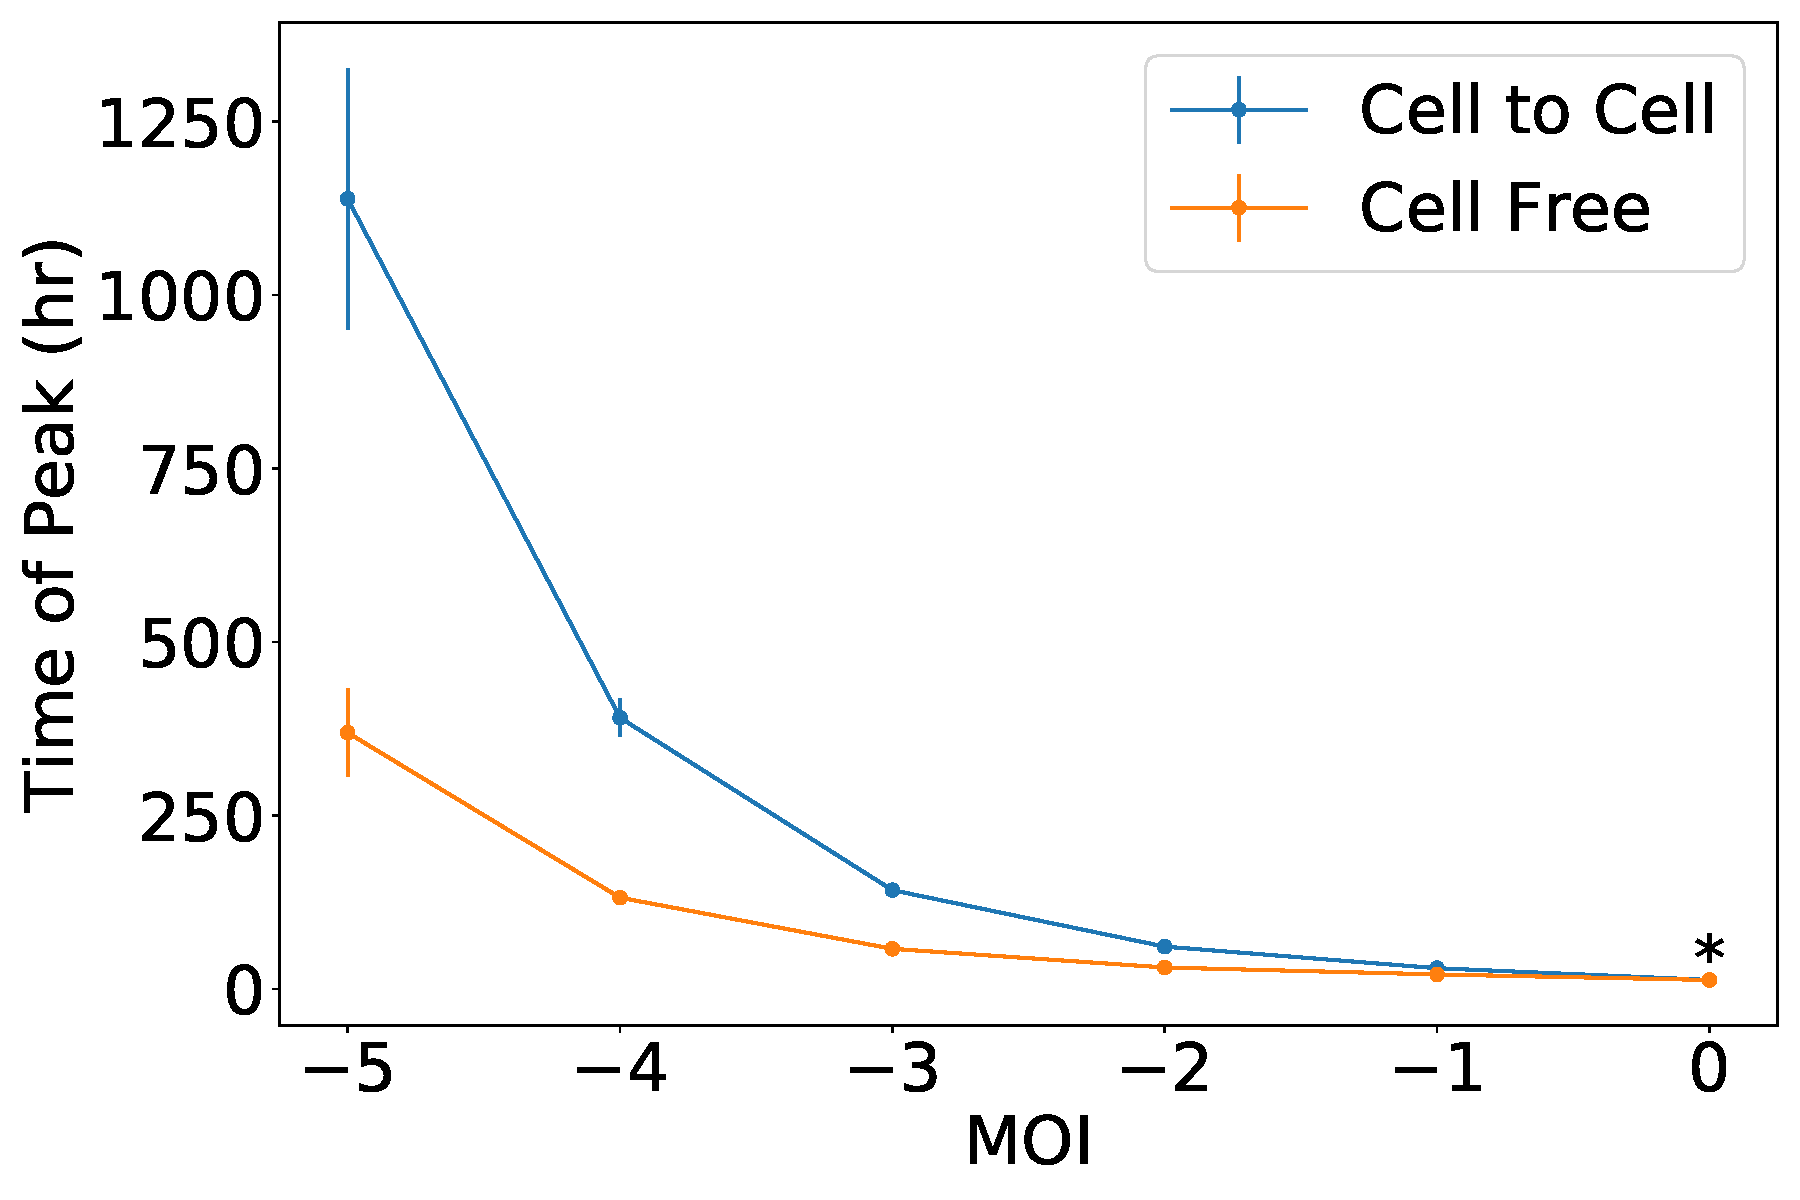
\includegraphics{Graphs/PeakViralTitterTimevsMOI.pdf}}}
    \onslide<4->{\resizebox{0.4\linewidth}{!}{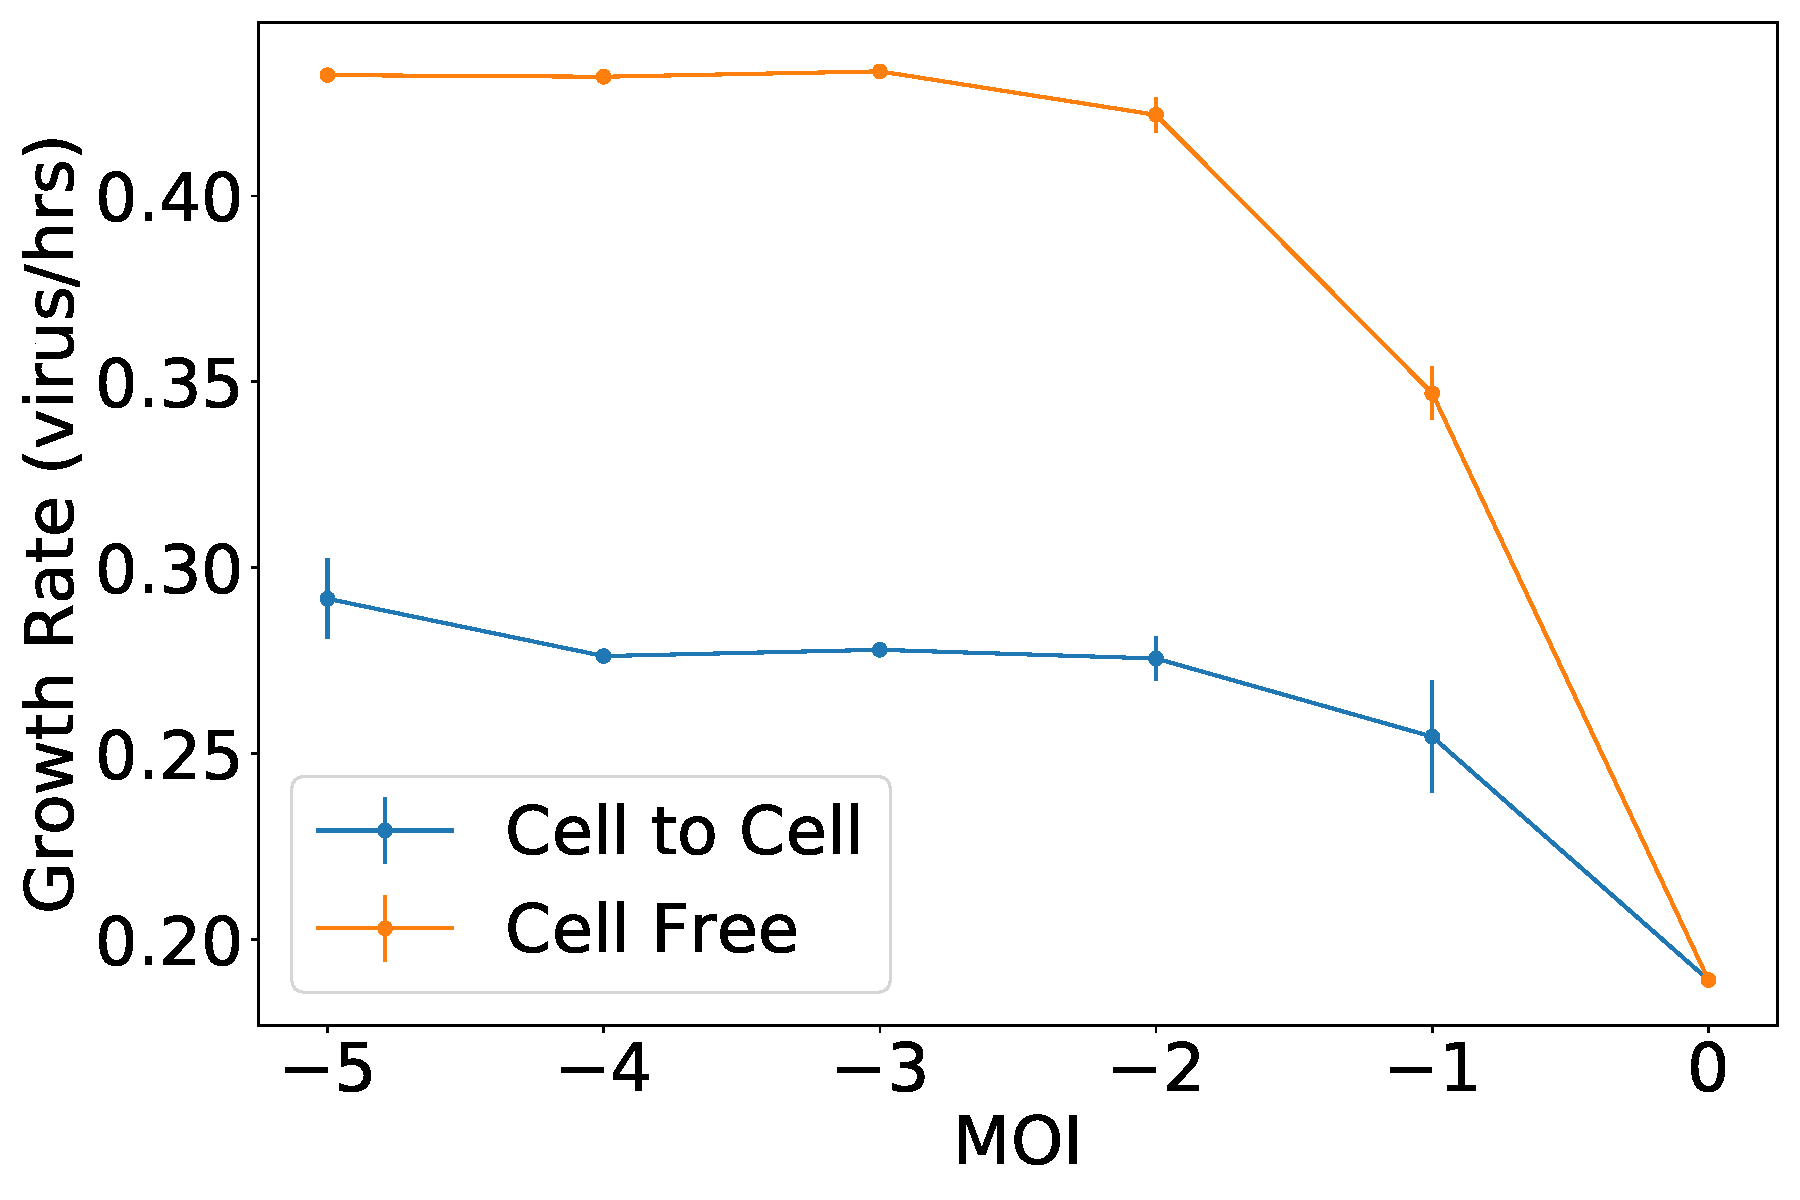
\includegraphics{Graphs/UpSlopevsMOI.pdf}}}
    \onslide<5->{\resizebox{0.4\linewidth}{!}{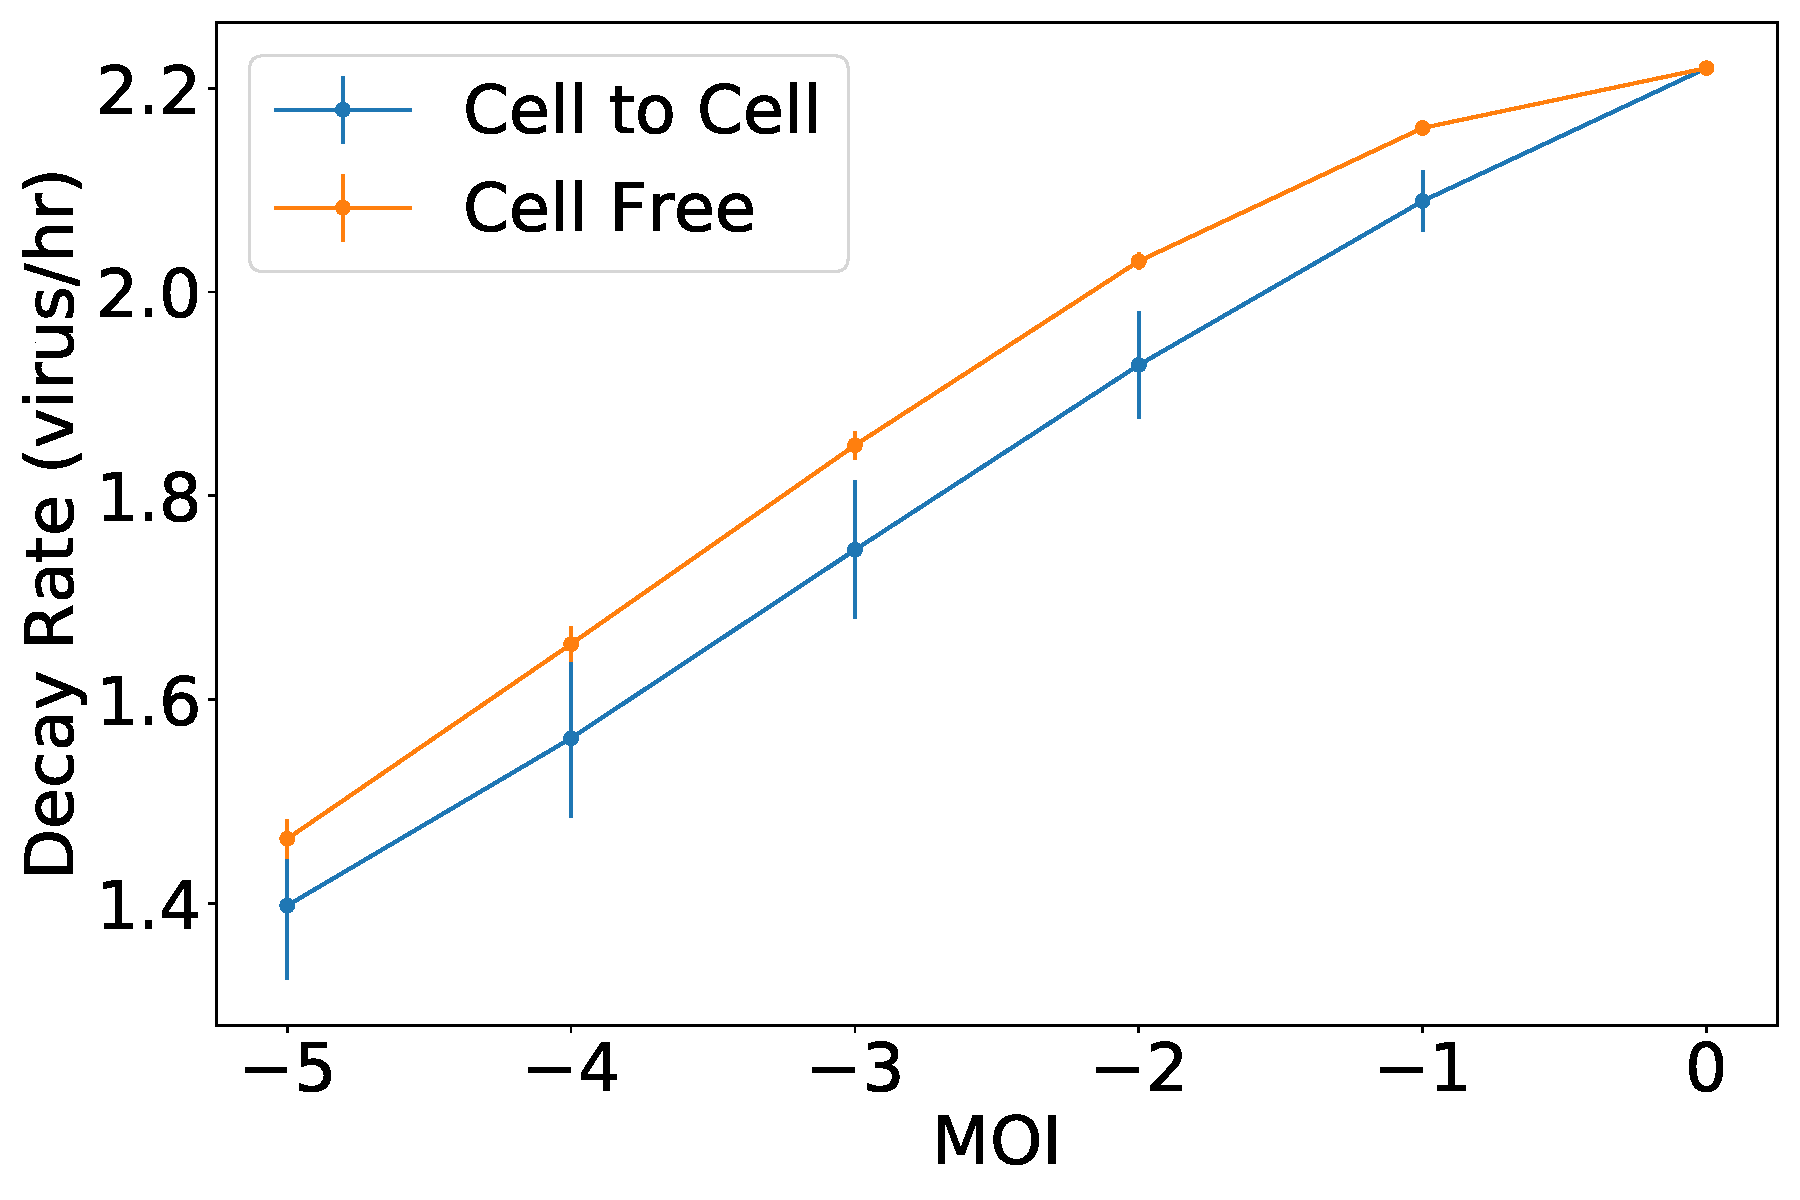
\includegraphics{Graphs/DownSlopevsMOI.pdf}}}
    \end{center}

\end{frame}

\begin{frame}{Timeline}

\begin{center}
\resizebox{1.0\linewidth}{!}{
\begin{tikzpicture}[timespan={}]
   \timeline[custom interval=true]{Summer 2020, Fall 2020, \shortstack[c]{Spring/\\Summer 2021}, Fall 2021, Spring 2022, Fall 2022, Spring 2023}
   \begin{phases}
     \initialphase{involvement degree=0cm,phase color=white}
     \phase{between week=1 and 2 in 0.0,
       involvement degree=3cm,phase color=yellow!90!red}
     \phase{between week=2 and 3 in 0.0,
       involvement degree=3cm,phase color=red!60!yellow}
     \phase{between week=3 and 4 in 0.0,
       involvement degree=3cm,phase color=lime}
     \phase{between week=4 and 5 in 0.0,
       involvement degree=3cm,phase color=red!60!yellow}
     \phase{between week=5 and 6 in 0.0,
       involvement degree=3cm,phase color=green!90!yellow}
     \phase{between week=6 and 7 in 0.0,
       involvement degree=3cm,phase color=red!60!yellow}
     \phase{between week=6 and 7 in 1.0,
       involvement degree=3cm,phase color=green!90!yellow}
   \end{phases}
   \node [xshift=-0.9cm,yshift=1cm,anchor=east,
          font=\Large\bfseries] at (phase-0.180) {\shortstack[c]{Writing and\\Researching}};
   \node [xshift=-0.6cm,yshift=-1.1cm,anchor=east,
          font=\Large\bfseries] at (phase-0.180) {\shortstack[c]{Defending and\\Submitting}};
   \begin{scope}{text options={above}}
     \onslide<2->{\addmilestone{at=phase-1.90,direction=90:3cm,
       text={\large\fcolorbox{white}{white}{\shortstack[c]{Run simulations\\with varying\\cell to cell probability}}}}}
     \onslide<5->{\addmilestone{at=phase-2.90,direction=90:1cm,
       text={\large\fcolorbox{white}{white}{\shortstack[c]{Compare cell to cell\\results to experiment,\\prepare manuscript}}}}}
     \onslide<7->{\addmilestone{at=phase-3.90,direction=90:3cm,
       text={\large\fcolorbox{white}{white}{\shortstack[c]{Run syncytia\\formation simulations}}}}}
     \onslide<9->{\addmilestone{at=phase-4.90,direction=90:1cm,
       text={\large\fcolorbox{white}{white}{\shortstack[c]{Prepare and test code\\with advection}}}}}
     \onslide<11->{\addmilestone{at=phase-5.90,direction=90:3cm,
       text={\large\fcolorbox{white}{white}{\shortstack[c]{Run advection\\simulations}}}}}
     \onslide<13->{\addmilestone{at=phase-6.105,direction=105:1cm,
       text={\large\fcolorbox{white}{white}{\shortstack[c]{Prepare advection\\manuscript}}}}}
     \onslide<14->{\addmilestone{at=phase-6.65,direction=65:3cm,
       text={\large\fcolorbox{white}{white}{\shortstack[c]{Write\\dissertation}}}}}
   \end{scope}
   \begin{scope}{text options={below}}
     \onslide<3->{\addmilestone{at=phase-1.235,direction=235:3cm,
       text={\large\fcolorbox{white}{white}{\shortstack[c]{Submit article\\on effect of\\multiplicity of infection}}}}}
     \onslide<4->{\addmilestone{at=phase-1.285,direction=285:1cm,
       text={\large\fcolorbox{white}{white}{\shortstack[c]{Submit computer\\science article}}}}}
     \onslide<6->{\addmilestone{at=phase-2.270,direction=270:3cm,
       text={\large\fcolorbox{white}{white}{\shortstack[c]{Defend\\Masters}}}}}
     \onslide<8->{\addmilestone{at=phase-3.270,direction=270:1cm,
       text={\large\fcolorbox{white}{white}{\shortstack[c]{Submit cell to cell\\paper}}}}}
     \onslide<10->{\addmilestone{at=phase-4.270,direction=270:3cm,
       text={\large\fcolorbox{white}{white}{\shortstack[c]{Prepare syncytia\\manuscript}}}}}
     \onslide<12->{\addmilestone{at=phase-5.270,direction=270:1cm,
       text={\large\fcolorbox{white}{white}{\shortstack[c]{Submit syncytia\\manuscript}}}}}
     \onslide<15->{\addmilestone{at=phase-7.250,direction=250:3cm,
       text={\large\fcolorbox{white}{white}{Defend Ph.D}}}}
     \onslide<16->{\addmilestone{at=phase-7.290,direction=290:1.5cm,
       text={\large\fcolorbox{white}{white}{\shortstack[c]{Submit advection\\manuscript}}}}}
   \end{scope}
\end{tikzpicture}}
\end{center}

\end{frame}

%-----------------------------------------------------------------------------------
\miniframesoff
    \section{}

\begin{frame}{Acknowlegdements}

    \begin{itemize}
        \item<2-> Dr. Dobrovolny
        \item<3-> Committee
        \item<4-> Faculty
        \item<5-> Grad-students
        \item<6-> Kelli
        \item<7-> Mom
        \item<8-> Corduroy \& Berry
        \item<9-> TCU Counseling and Mental Health Center 
    \end{itemize}

\end{frame}

\begin{frame}{}

\begin{center}
\Huge Thank You
\end{center}

\end{frame}


\miniframesoff
    \section{}

%Extra
\begin{frame}{}
    %Blank
\end{frame}

\begin{frame}{Quantal Assays}

    \resizebox{1.0\linewidth}{!}{\begin{columns}
    \column{0.45\textwidth}
    \begin{itemize} 
        \item Multi-well plates
        \begin{itemize}
            \item different groups of wells on the plate are filled with a dilution of virus that often varies in a ten fold difference from group to group.
        \end{itemize}
    \end{itemize}

    \column{0.45\textwidth}
    \begin{itemize} 
        \item Animals
        \begin{itemize}
            \item different animal subjects are injected with a dilution of virus that often varies in a ten fold difference from subject to subject. 
        \end{itemize}
    \end{itemize}
    \end{columns}}

\end{frame}

\begin{frame}{Choice in model vs. experiment}

    \begin{itemize}
        \item The use of assays is crucial to studying viruses, but they do have some limitations. 
        \item Performing many assays requires a lot of funds, labor, and time to make the different measurements for analysis. 
        \begin{itemize}
            \item This leads to either data not being collected as often as might be necessary or not enough cases being studied to capture all of the fine details of an infection. 
        \end{itemize}
        \item Another difficulty with assays is that some characteristics of viruses cannot be controlled for in experiments. 
        \begin{itemize}
            \item For example, it's difficult to stop all of the cell to cell transmission or all of the cell free transmission. 
            \item This makes it impossible to have an isolated study of one characteristic of an infection. 
        \end{itemize}
        \item By using computer models, many cases with more frequent data collection can be performed using fewer resources.
    \end{itemize}

\end{frame}

\begin{frame}{}
    \begin{center}
        SARS-CoV-2 transmits easier then SAR's
    \end{center}
\end{frame}

\begin{frame}{}
    \begin{center}
        \resizebox{1.0\linewidth}{!}{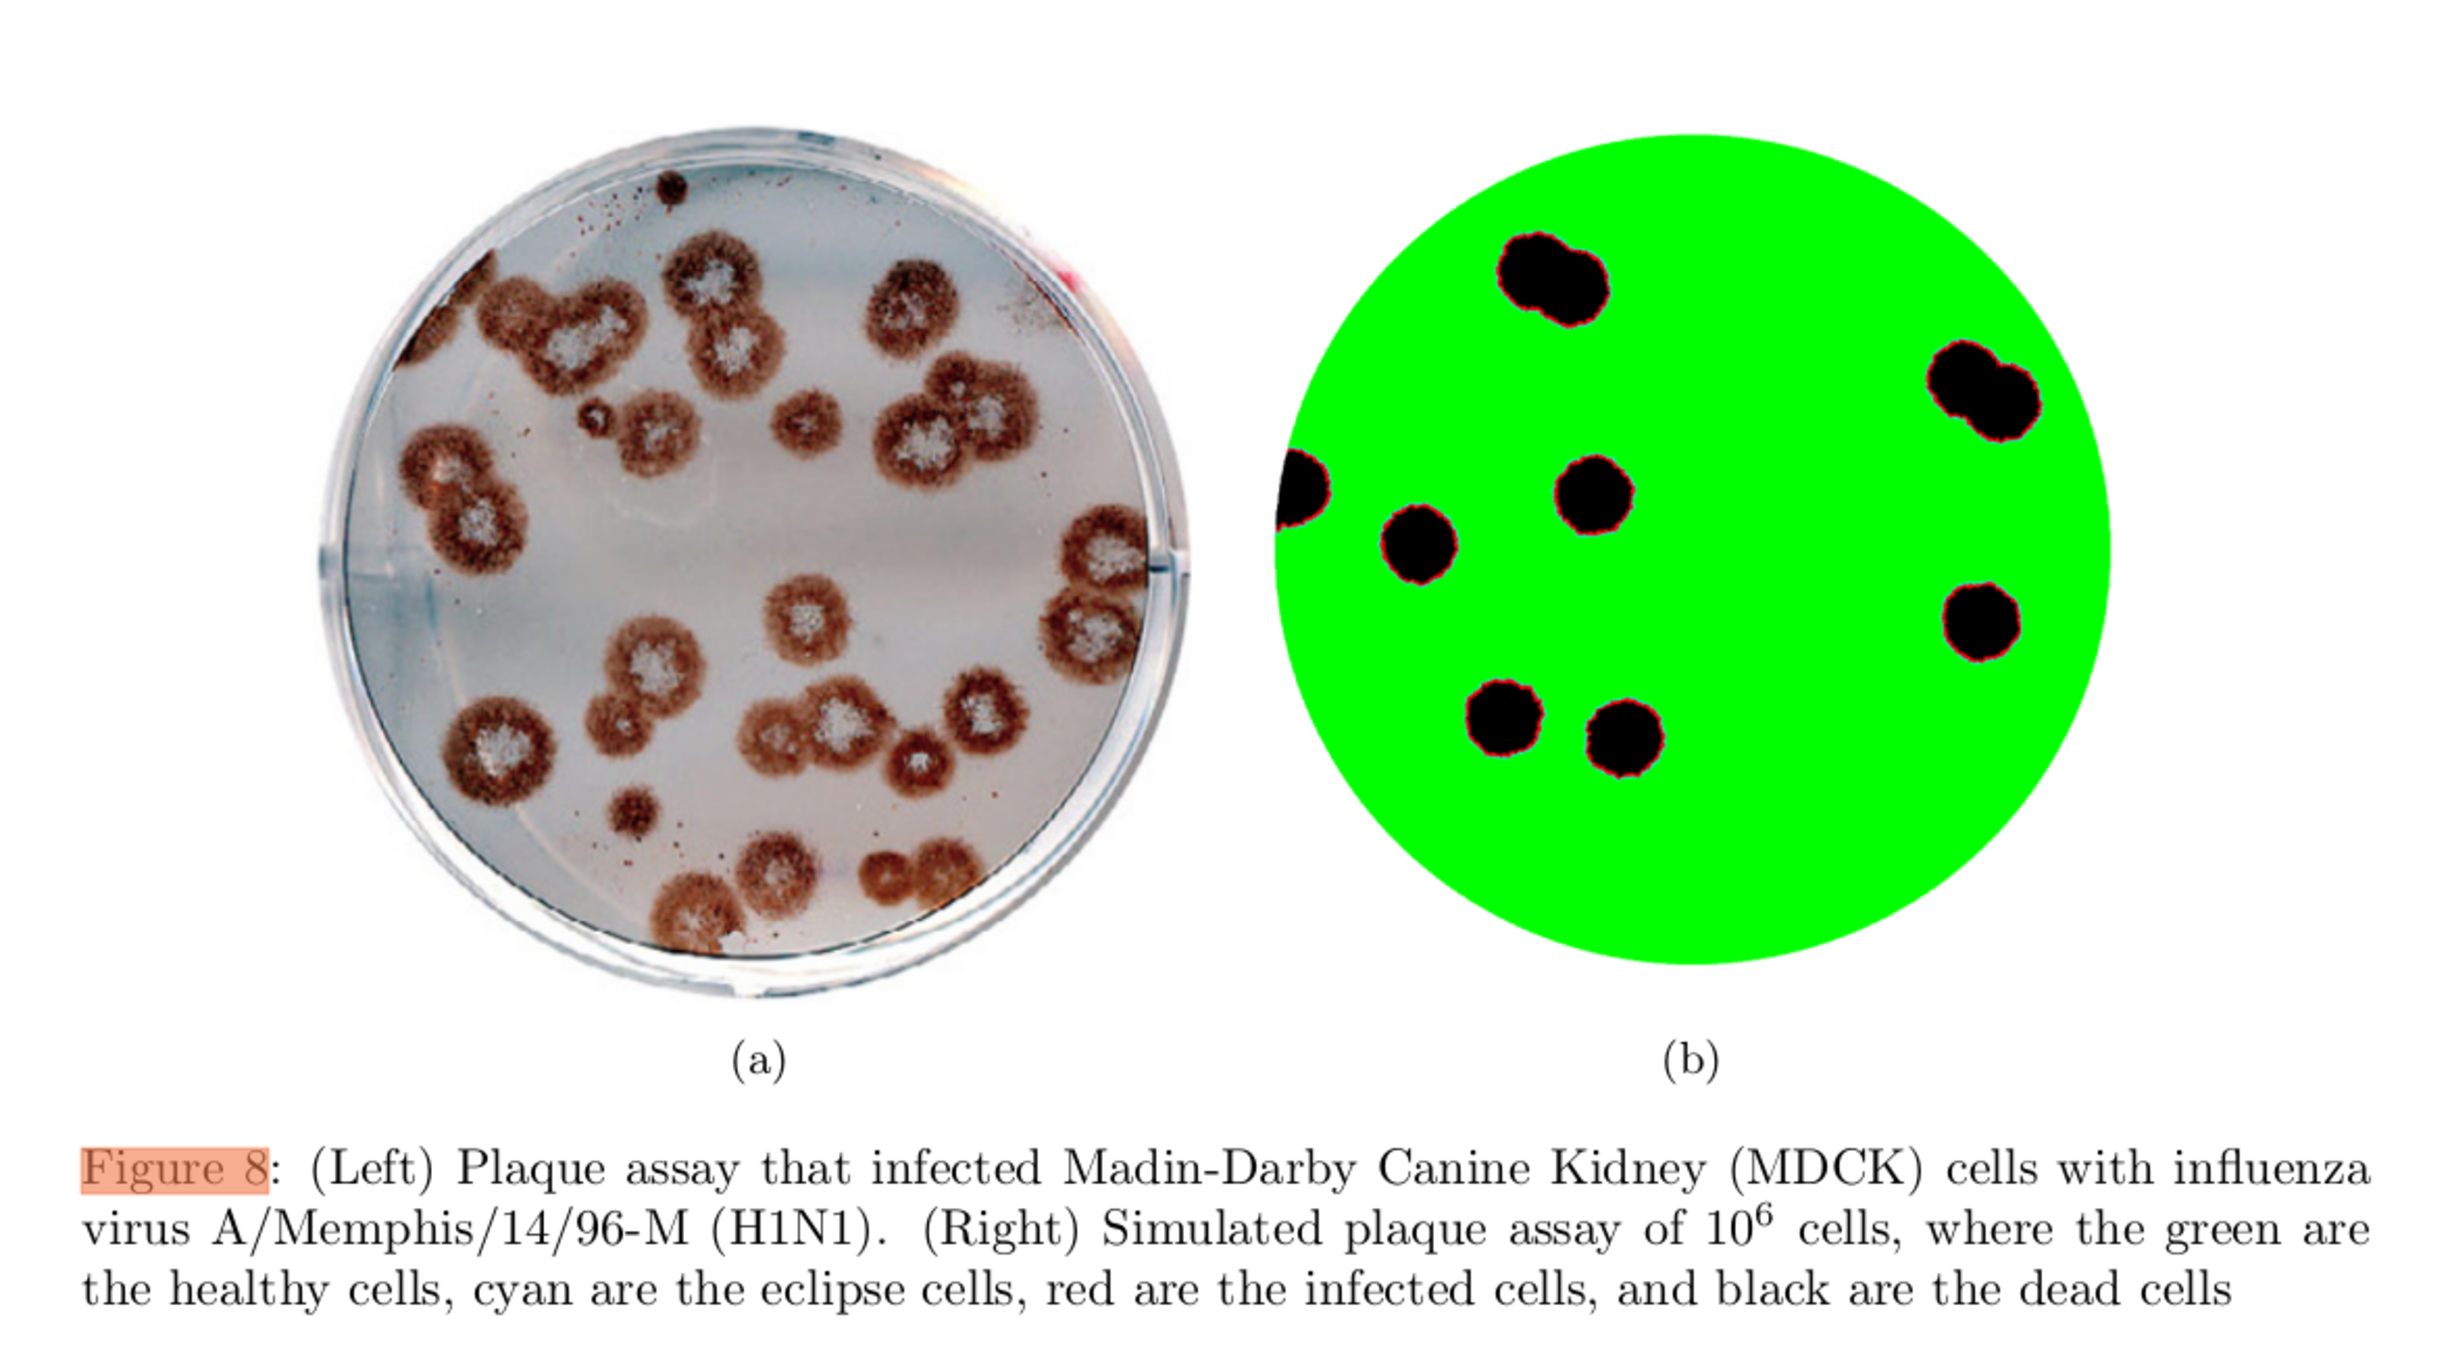
\includegraphics{Images/Figure_8.pdf}}
    \end{center}
\end{frame}

\begin{frame}{Immune Response}
    \begin{center}
        \begin{itemize}
            \item Slide about how immune response could be implemented
            \item Papers about ABM
            \item Know major components
            \item Complicated to do - not alot of data
            \item Stephaine Forrest
        \end{itemize}
    \end{center}
\end{frame}

\begin{frame}{Python vs C vs CUDA}
    \begin{center}
        \begin{itemize}
            \item Python is an interpreted, object-oriented, high-level programming language with dynamic semantics.
            \item The C programming language is a computer programming language that was developed to do system programming for the operating system UNIX and is an imperative programming language.
            \item CUDA (Compute Unified Device Architecture) is a parallel computing platform and application programming interface (API) model created by Nvidia

        \end{itemize}
    \end{center}
\end{frame}

\begin{frame}{Python vs C vs CUDA}
    \begin{center}
        \begin{itemize}
            \item Python easy to read, easy to write, but can be slow, often does not allow for memory control
            \item C hard to learn, easy to write; can be very fast, allows for total memory control
            \item CUDA have to understand c/c++ in order to write cuda, very difficult to write if new to the idea of parallelization. Have to understand memory allocation. For larger numbers of calculations is can get hundreds of times speed up. 

        \end{itemize}
    \end{center}
\end{frame}

\begin{frame}{Python vs CUDA speed up}
    \begin{center}
        \begin{itemize}
            \item Python - 21 hour per 24 hour of simulated time
            \item CUDA - 24 sec per  24 hour of simulated time
        \end{itemize}

        \begin{itemize}
            \item 3150 times speedup
        \end{itemize}
    \end{center}
\end{frame}

\begin{frame}{}
    \begin{center}
        $\mathcal{O}(n\log_{10} (n))$

    \begin{itemize}
        \item The $n$ comes from the loop for all of the cells
        \item The $\log_{10} (n)$ comes from division by 2 in the adaptive time step used in the cell free transmission
    \end{itemize}
    \end{center}
\end{frame}

\begin{frame}{Gamma Distribution}
    \begin{center}
    \begin{itemize}
        \item If k is a positive integer, then the distribution represents an Erlang distribution
        \item $y$ is distributed from $\mathrm{gamma}(\alpha, \beta)$
        \begin{itemize}
            \item If it has a corresponding pdf $P(y|\alpha, \beta) = \frac{\beta^{\alpha}}{\Gamma(\alpha)} y^{\alpha-1} e^{-\beta y}$
            \item continuous distribution
            \item $\alpha, \beta >0$ and $y \geq 0$ 
        \end{itemize}
        \item Used for a mean measure of a count variable
        \begin{itemize}
            \item using gamma as inputs to a Poisson distribution, because $\lambda$ of Poisson distro. is defined as $\lambda \geq 0$
        \end{itemize}
        \item Increase $alpha$ moves hump along the positive x-axis
        \item Increase $beta$ sharpens the peak
    \end{itemize}
        Ben Holder
        
    \end{center}
\end{frame}

\begin{frame}{Mean of Gamma Distribution}
    \begin{center}
    \begin{itemize}
        \item $P(y|\alpha, \beta) = \frac{\beta^{\alpha}}{\Gamma(\alpha)} y^{\alpha-1} e^{-\beta y}$
        \item $E[y] = \frac{\beta^{\alpha}}{\Gamma(\alpha)} \int^{\infty}_0 y^{\alpha} e^{-\beta y} dy$
        \item $E[y] = \frac{\beta^{\alpha}}{\Gamma(\alpha)} \frac{\gamma(\alpha+1)}{\beta^{\alpha+1}} \int^{\infty}_0 \frac{\beta^{\alpha+1}}{\gamma(\alpha+1)} y^{\alpha} e^{-\beta y} dy$
        \item $\int^{\infty}_0 \frac{\beta^{\alpha+1}}{\gamma(\alpha+1)} y^{\alpha} e^{-\beta y} dy = 1$
        \item $E[y] = \frac{\beta^{\alpha}}{\Gamma(\alpha)} \frac{\gamma(\alpha+1)}{\beta^{\alpha+1}}$
        \item $E[y] = \frac{\alpha}{\beta}$
    \end{itemize}
        
    \end{center}
\end{frame}

\begin{frame}{}
    \begin{center}
    \begin{itemize}
        \item $u(x,t)$ Concentration of particles in pipe; unit: mass/length
        \item $M = u(x,t) \Delta x$; aproximate mass is a volume of pipe $\Delta x$ long
        \item $\frac{dM}{dt} = J(x,t) - J(x+\Delta x, t)$; where $J$ is the flux
        \item $J(x,t) = -D u_x(x,t)$ Fick's law of diffusion; Units of D are $lenght^2$/time
        \item Now we can write
        \item $u(x,t) \Delta x = D(u_x(x+ \Delta x,t) - u_x(x,t))$
        \item $u(x,t) = \frac{D(u_x(x+ \Delta x,t) - u_x(x,t))}{\Delta x}$
        \item Taking the limit as $\Delta x \to 0$
        \item $u(x,t) = Du_xx$
    \end{itemize}
    \end{center}
\end{frame}

\begin{frame}{Fick's first law of diffusion}
    \begin{center}
    \begin{itemize}
        \item The simplest description of diffusion is given by Fick's laws, which were developed by Adolf Fick in the 19th century:
        \begin{itemize}
            \item The molar flux due to diffusion is proportional to the concentration gradient.
            \item Writing the first law in a modern mathematical form:
            \item $N_i = -D_i \nabla c_i$
            \item where for species i, $N_i$ is the molar flux (mol $m^{-2}$ $s^{-1}$), $D_i$ is the diffusion coefficient ($m^2$ $s^{-1}$), and $c_i$ is the concentration (mol $m^{-3}$).

            \item From the continuity equation for mass:
            \item $\frac{\partial c_i}{\partial t}+\nabla \cdot N_i =0$
            \item we can derive Fick's second law directly:
            \item $\frac{\partial c_i}{\partial t} = D_i \nabla^2 c_i$
            \item This assumes that Di is a constant, which is only true for dilute solutions. This is usually a good assumption for diffusion in solids; diffusion of chemicals in a dilute solution, water, or other typical liquid solvents; and diffusion of dilute (trace) species in the gas phase, such as carbon dioxide in air.
        \end{itemize}
    \end{itemize}
        
    \end{center}
\end{frame}

\begin{frame}{}
    \begin{center}
        Boundary conditions
%        $a\frac{\partial C}{\partial t} = \mp D\frac{\partial C}{\partial x}$
        
    \end{center}
\end{frame}

\begin{frame}{}
    \begin{center}
        \resizebox{1.0\linewidth}{!}{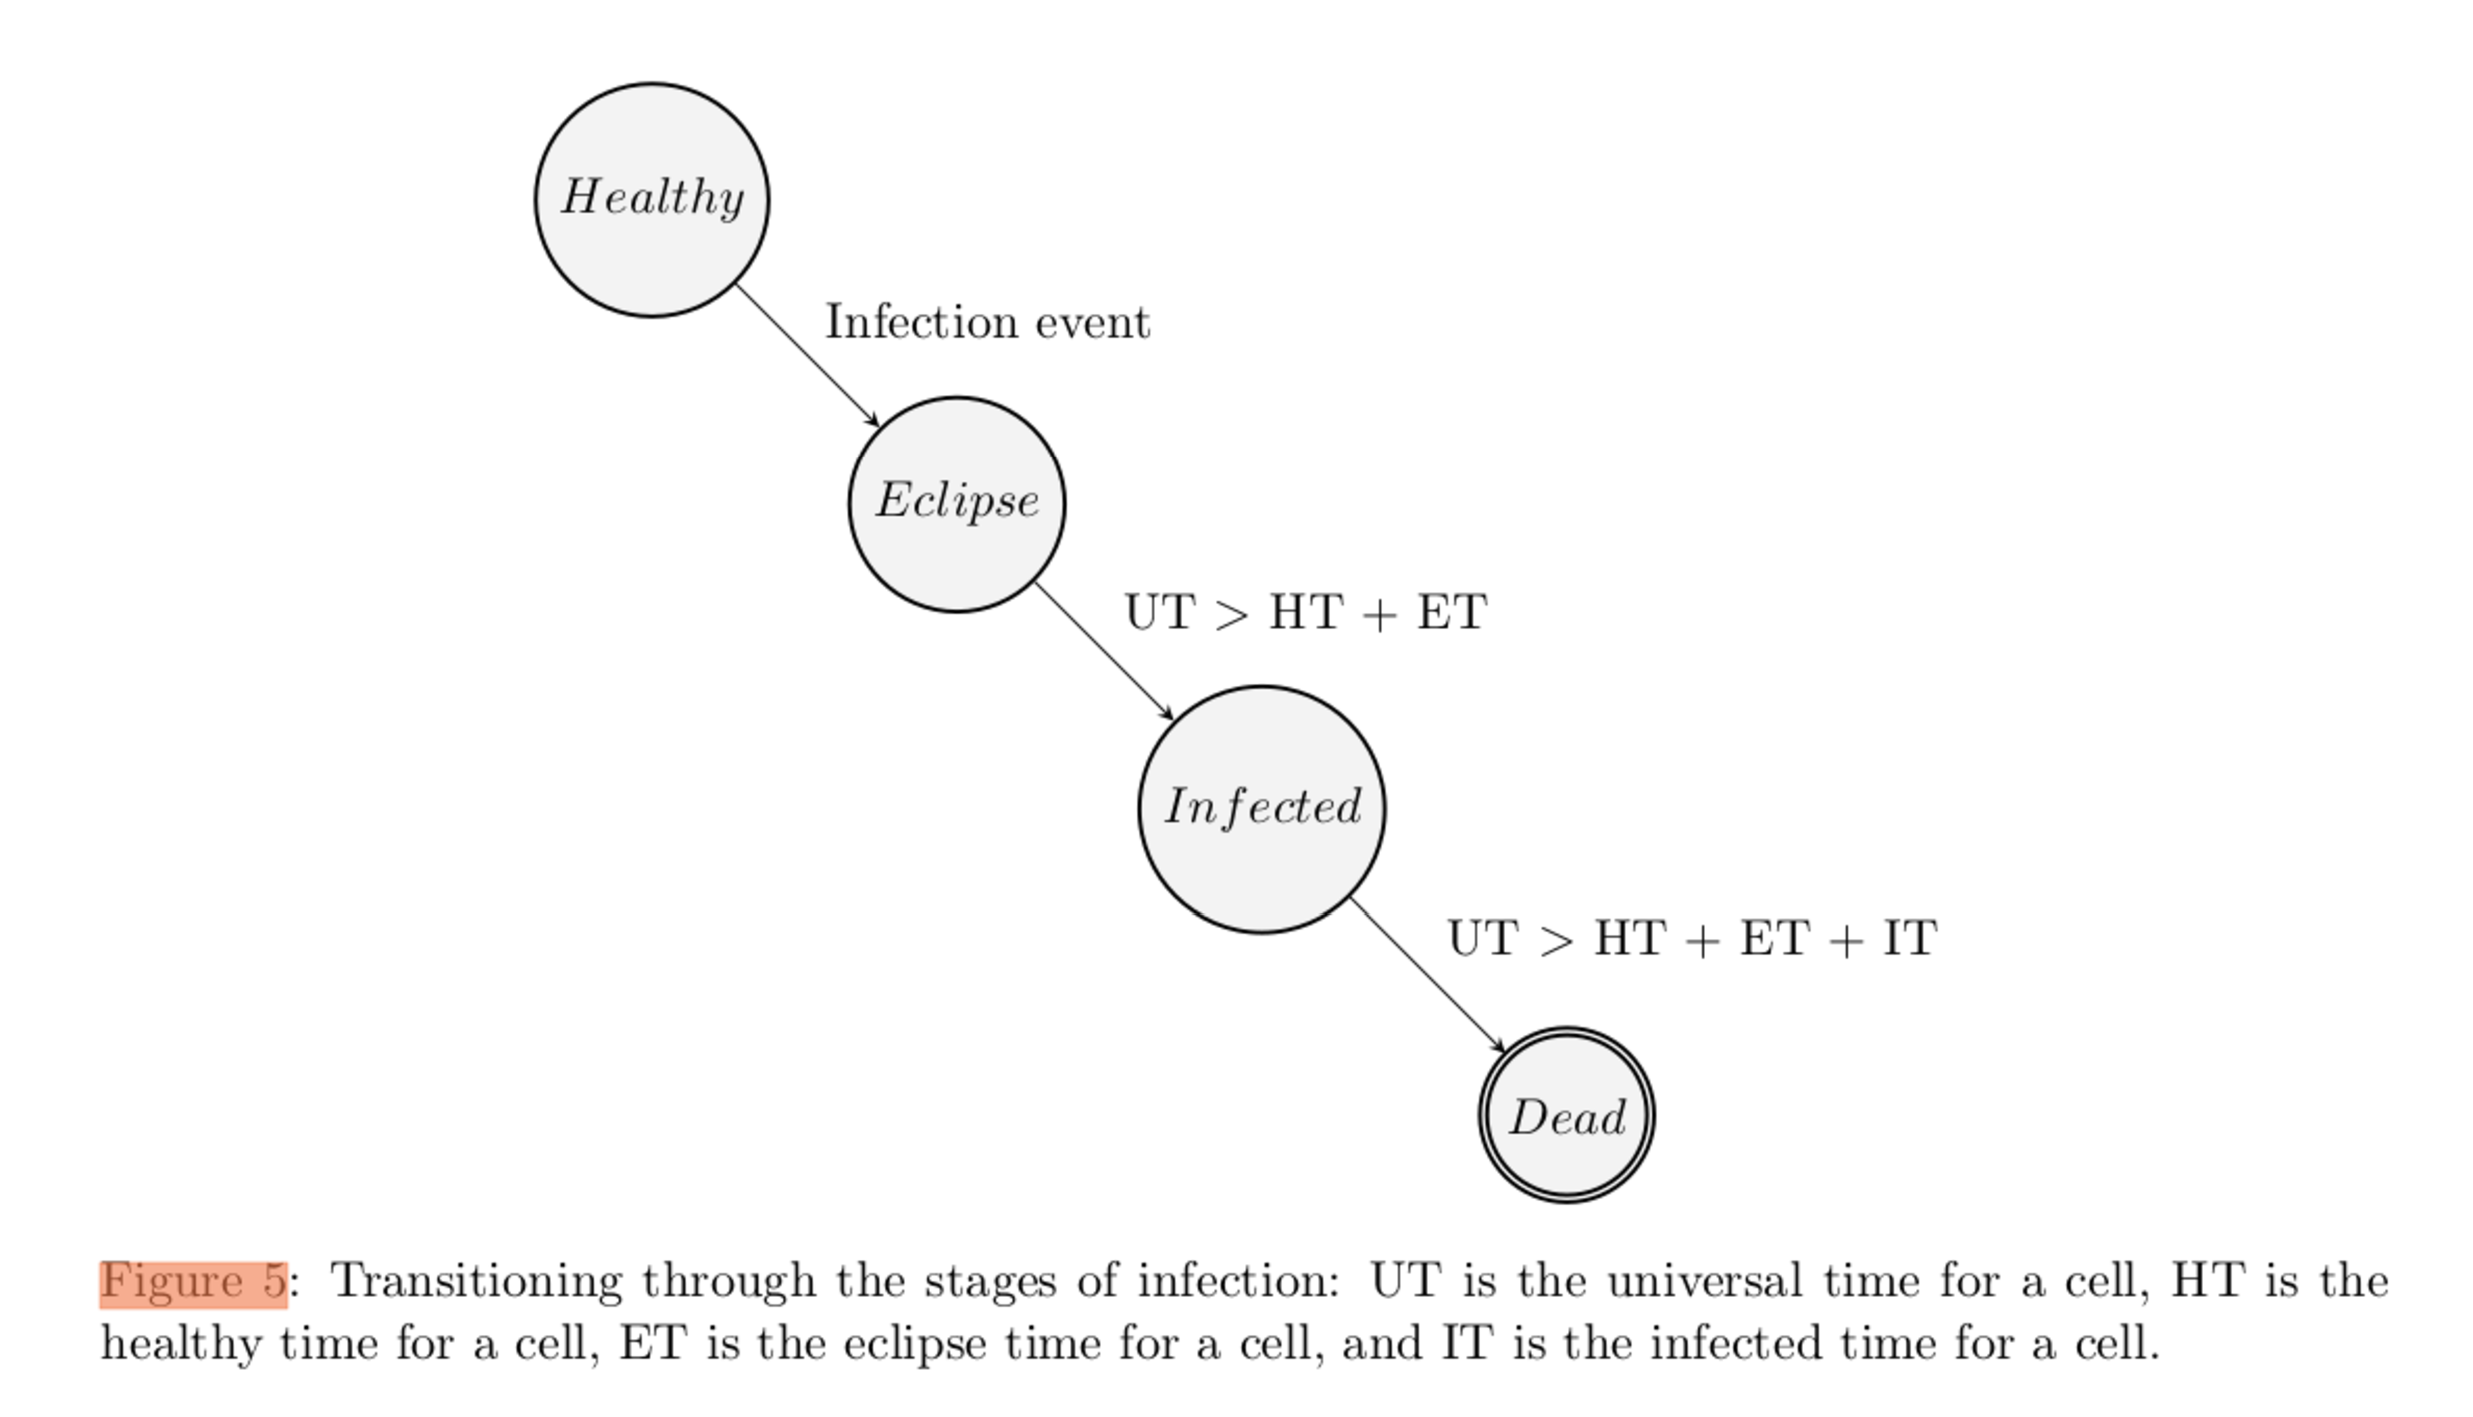
\includegraphics{Images/Figure_5.pdf}}
    \end{center}
\end{frame}

\begin{frame}{}
    \begin{center}
        \resizebox{1.0\linewidth}{!}{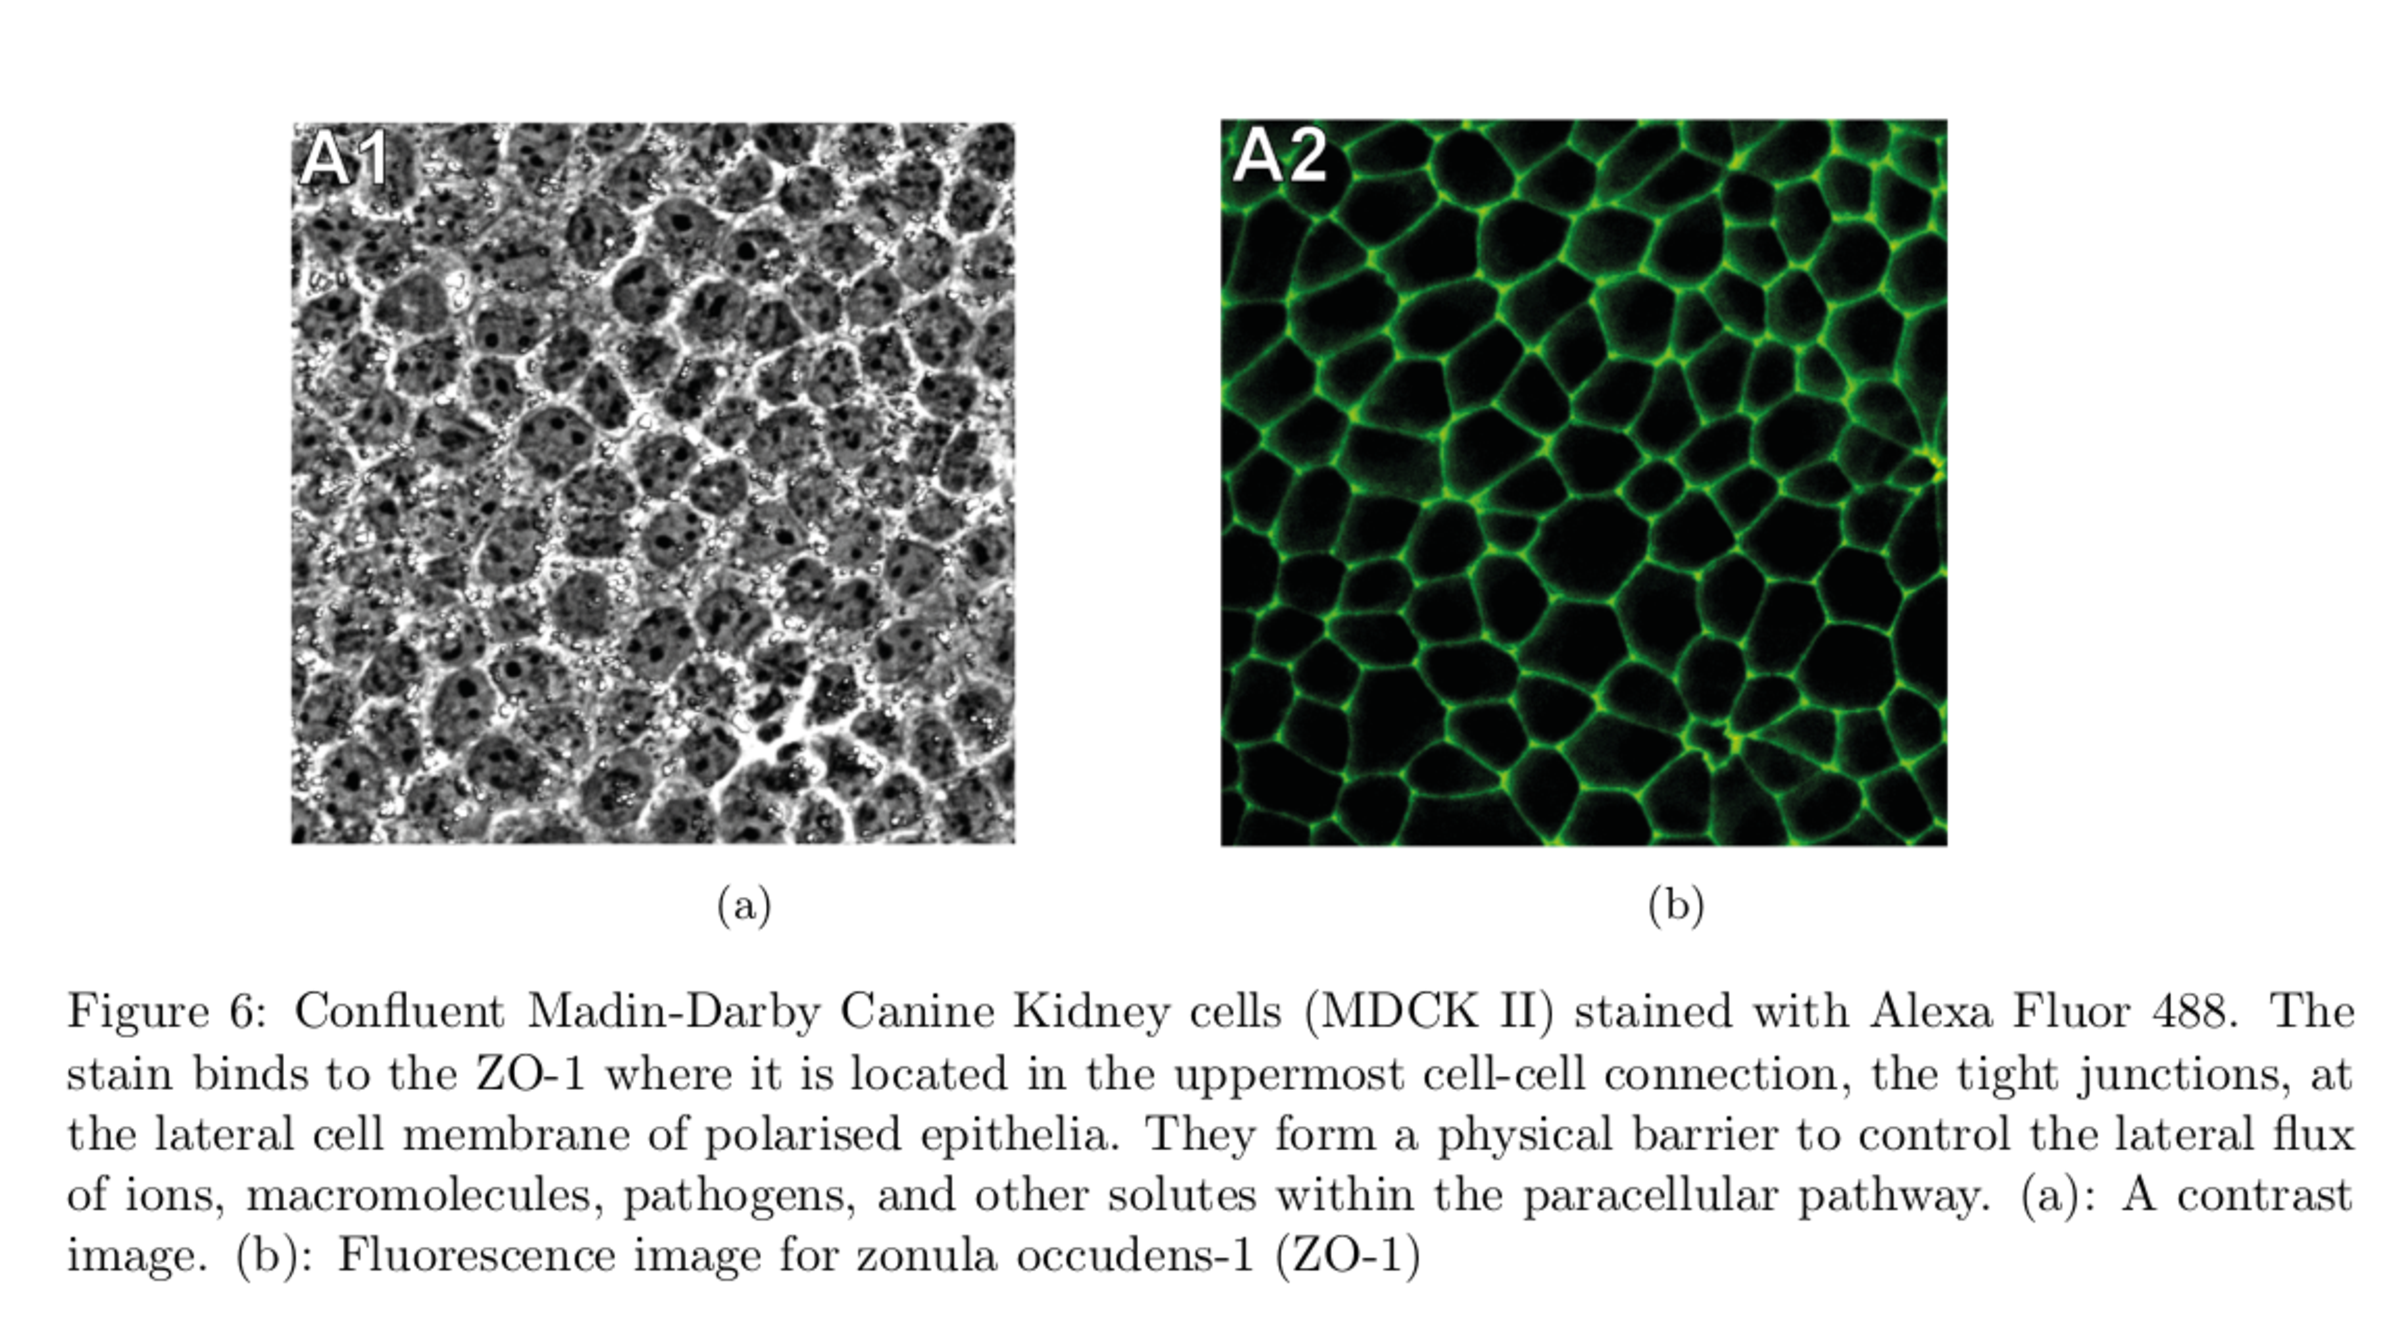
\includegraphics{Images/Figure_6.pdf}}
    \end{center}
\end{frame}

\begin{frame}{}
    \begin{center}
         \begin{itemize}
            \item $x = X_{hex}$
            \item $y = 2/3*\sin(\pi/3)*\left ( Y_{hex}-Z_{hex} \right )$
        \end{itemize}
\begin{enumerate} 
    \item The coordinates can be split in to three sectors where the coordinates $X_{hex}$, $Y_{hex}$, and $Z_{hex}$ are simply cyclic permutations.
    \item The $X_{hex}$ and $Z_{hex}$ coordinates, also known as axial coordinates, can be used as indices of a matrix.
    \item  The coordinates of the neighboring hexagons are found by adding a cyclic permutation of 
        $\left [
            \begin{array}{c}
                1 \\
                0 \\
                -1\\
            \end{array}
        \right ]$
        for three of the neighbors and
        $\left [ 
            \begin{array}{c}
                1 \\
                -1 \\
                0\\
            \end{array}
        \right ]$
        for the other three neighbors.
\end{enumerate}
        
    \end{center}
\end{frame}

\begin{frame}{}
    \begin{center}
        $$\frac{\partial V}{\partial t} = D\frac{2}{3} \left (\frac{\partial^2}{\partial x^2_1}+\frac{\partial^2}{\partial x^2_2}+\frac{\partial^2}{\partial x^2_3}\right )V$$ 
    \end{center}

Unit vectors 
\begin{itemize}
    \item $\textbf{x}_1=
\left [
    \begin{array}{c}
        1 \\
        0 \\
    \end{array}
\right ]$

    \item $\textbf{x}_2=
\left [
    \begin{array}{c}
        -1/2 \\
        \sqrt{3}/2 \\
    \end{array}
\right ]$

    \item $\textbf{x}_3=
\left [
    \begin{array}{c}
        -1/2 \\
        -\sqrt{3}/2 \\
    \end{array}
\right ]$
\end{itemize}

\end{frame}

\begin{frame}{}
    \begin{center}
        \resizebox{1.0\linewidth}{!}{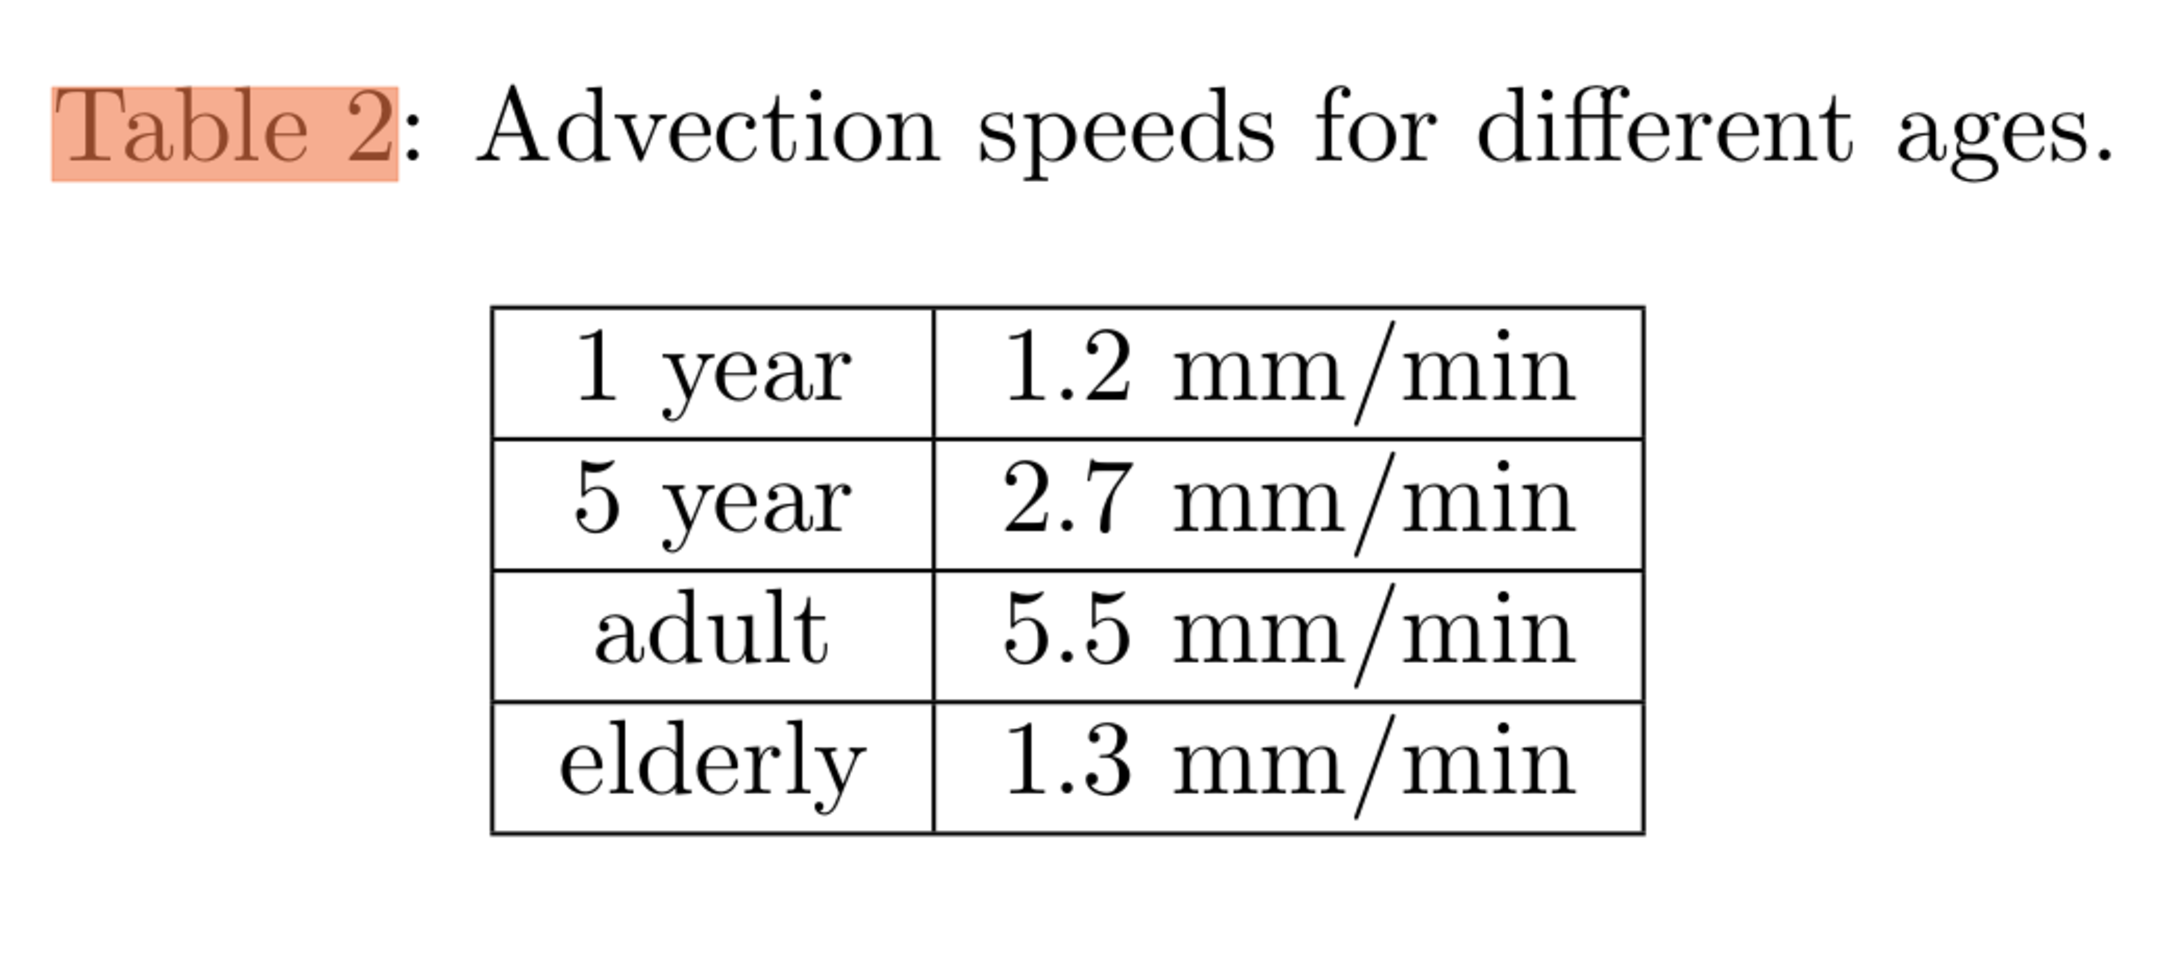
\includegraphics{Images/Table_2.pdf}}
    \end{center}
\end{frame}

\begin{frame}{}
    \begin{center}
        \resizebox{1.0\linewidth}{!}{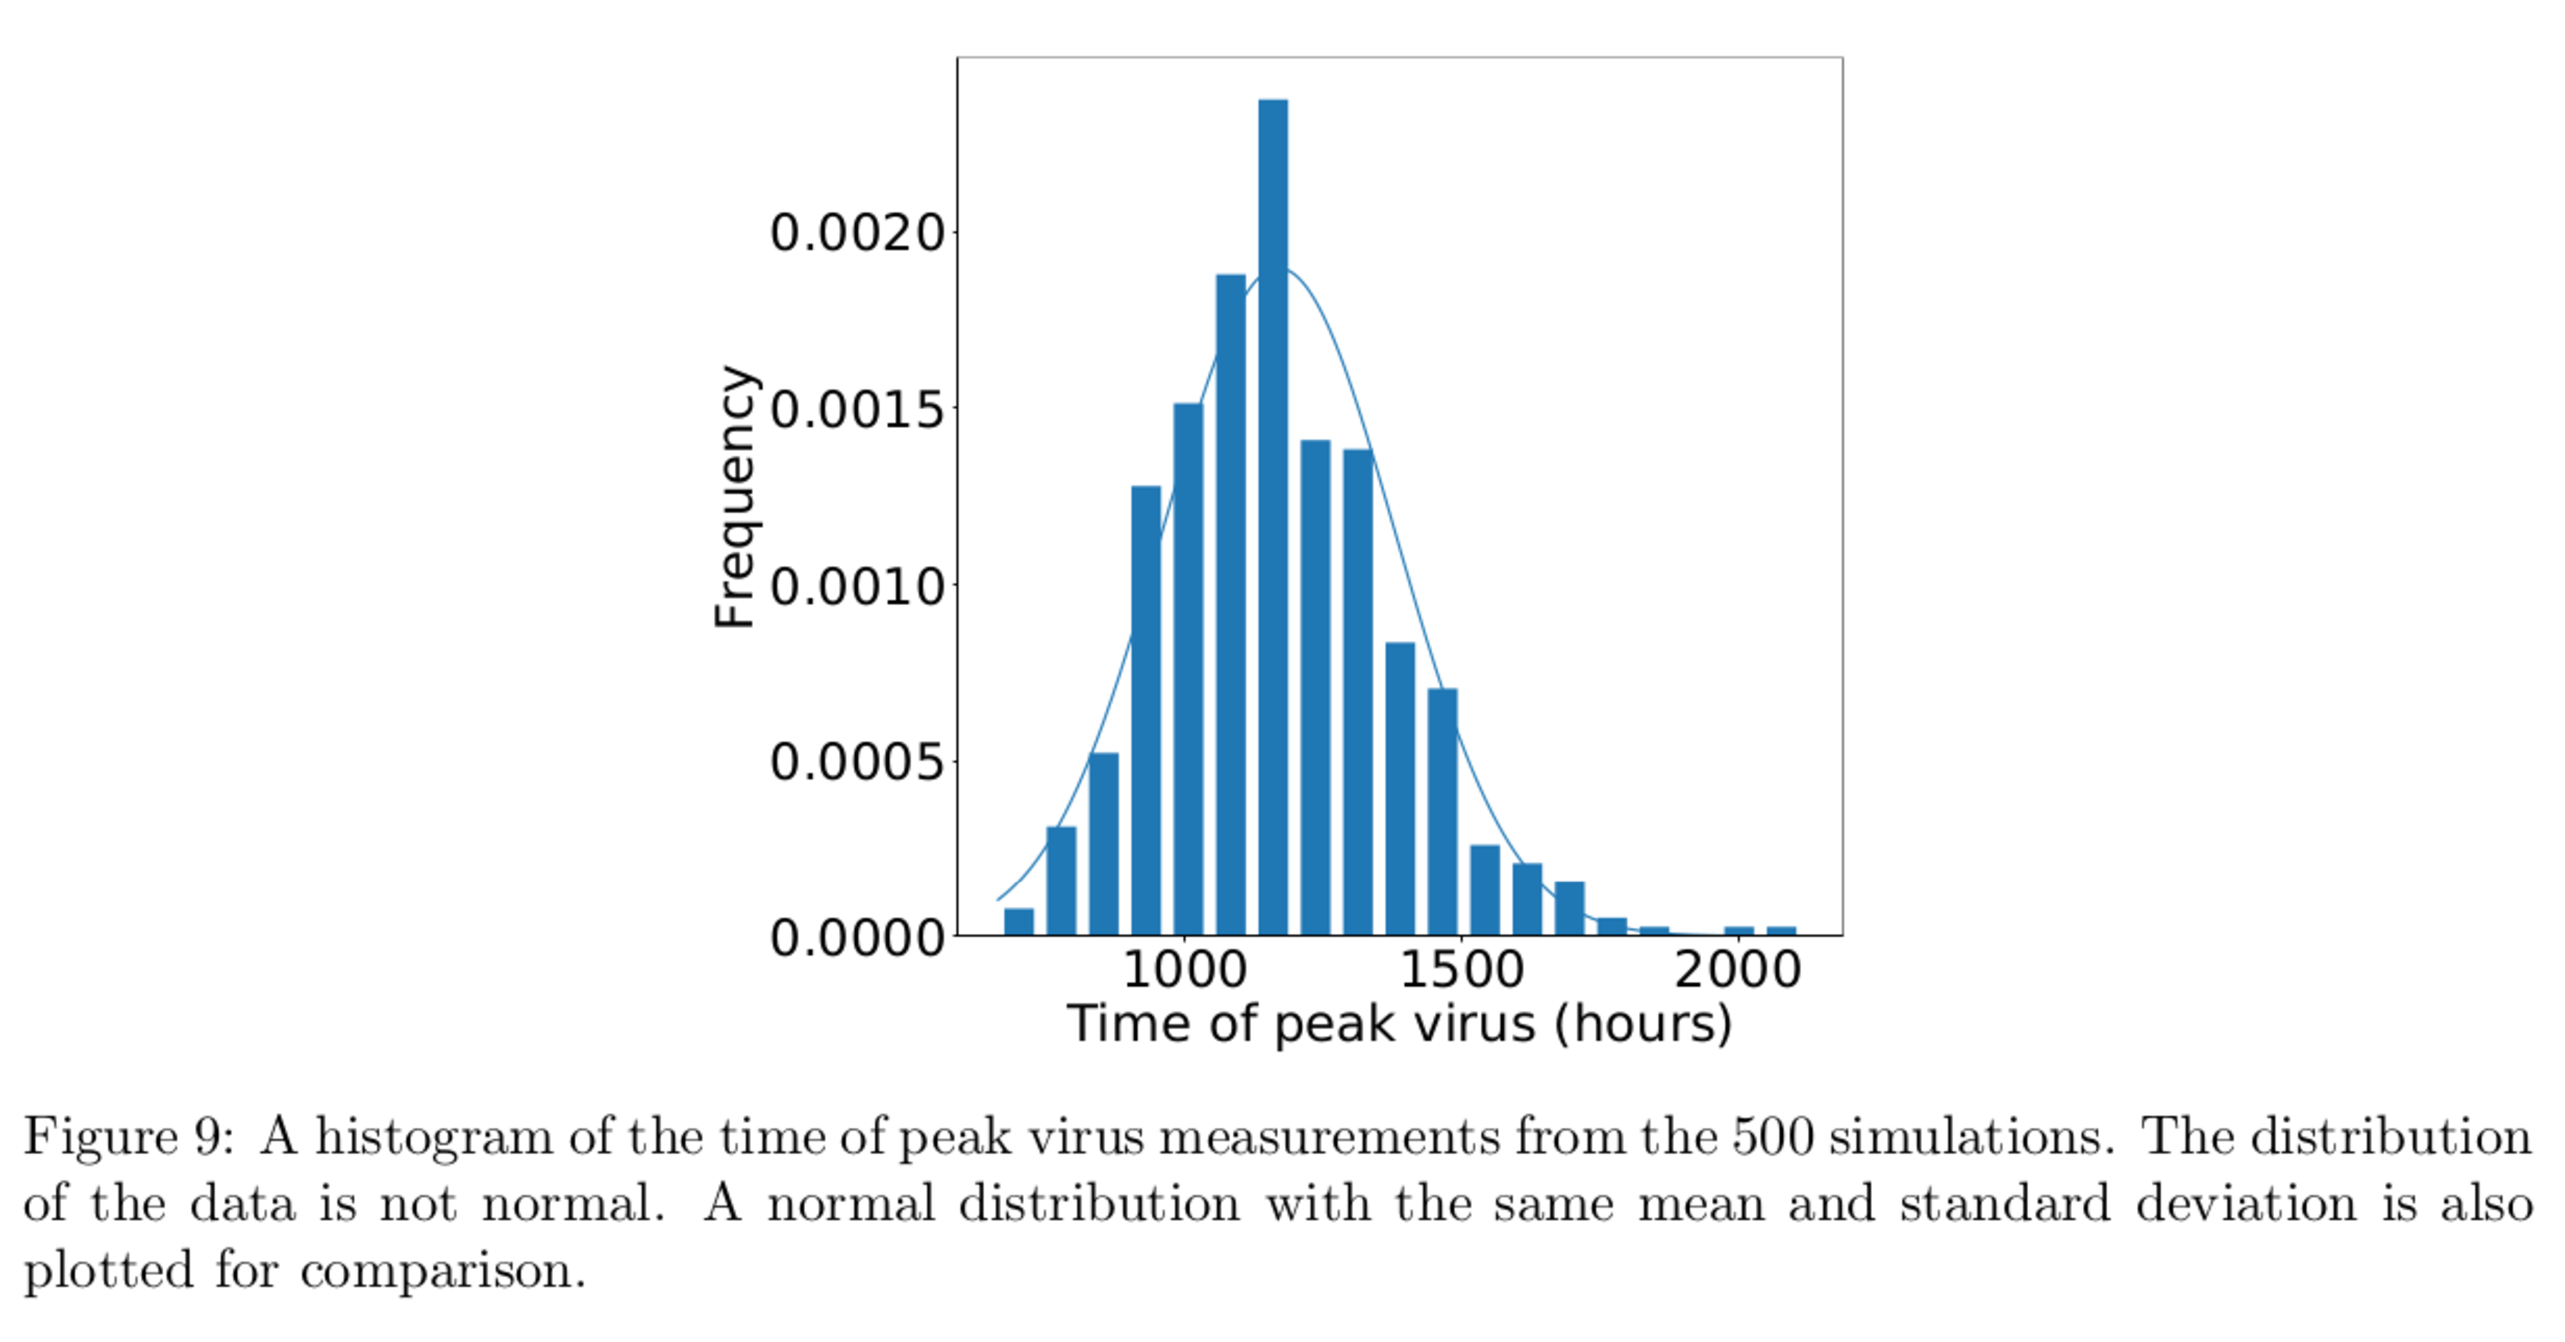
\includegraphics{Images/Figure_9.pdf}}
    \end{center}
\end{frame}

\begin{frame}{}
    \begin{center}
    \begin{itemize}
        \item density : bool, optional

        \item If False, the result will contain the number of samples in each bin. If True, the result is the value of the probability density function at the bin, normalized such that the integral over the range is 1. Note that the sum of the histogram values will not be equal to 1 unless bins of unity width are chosen; it is not a probability mass function. Overrides the normed keyword if given.
    \end{itemize}
    \end{center}
\end{frame}

\begin{frame}{}
    \begin{center}
        Test for normal
        U-Test
        T-Test
        Assumptions for tests
    \end{center}
\end{frame}

\begin{frame}{}
    \begin{center}
    \begin{itemize}
        \item Assumptions for tests
        \item Shapiro-Wilk
        \item D'Agostino's K-squared
        \item Anderson-Darling
    \end{itemize}
    \end{center}
\end{frame}

\begin{frame}{}
    \begin{center}
        Be familiar with results of MOI papers
        -maybe a slide of the main results
    \end{center}
\end{frame}

\begin{frame}{}
    \begin{center}
        \resizebox{1.0\linewidth}{!}{\includegraphics{Images/Table_4.pdf}}
    \end{center}
\end{frame}

\begin{frame}{}
    \begin{center}
        \resizebox{1.0\linewidth}{!}{\includegraphics{Images/Table_5.pdf}}
    \end{center}
\end{frame}

\begin{frame}{}
    \begin{center}
        Make some slides of the results of results of other papers
    \end{center}
\end{frame}

\begin{frame}{}
    \begin{center}
        What other viruses that C2C
        HIV
        HCV
        Check other modeling papers for virus
    \end{center}
\end{frame}

\begin{frame}{}
    \begin{center}
        More virus more transmission
        upslope - how bad you feel
        Time to peak
        Upslope         -   Duration
        Downslope
    \end{center}
\end{frame}

\end{document}
